\documentclass[aps,pra,11pt,onecolumn,nofootinbib,tightenlines]{revtex4-2}

\usepackage{mathrsfs}
\usepackage{graphicx}
\usepackage{comment}
\usepackage{dsfont}
\usepackage{amsmath}
\usepackage{amsfonts}
\usepackage{amssymb}
\usepackage{amsthm}
\usepackage{float}
\usepackage[colorlinks=true,urlcolor=blue,citecolor=blue,linkcolor=blue]{hyperref}
\usepackage{caption}
\captionsetup{justification=raggedright}
\usepackage{lipsum}
\usepackage{subcaption}
\usepackage{mwe}
\usepackage{enumerate}
\usepackage{sidecap}
\usepackage{natbib}
\usepackage{appendix}
\usepackage{tikz}
\usetikzlibrary{arrows.meta,positioning,fit}
\usepackage{booktabs}
\usepackage{longtable}
\usepackage{array}
\usepackage{multirow}
\usepackage{forest}
\usepackage{bm}
\usepackage{empheq}
\usepackage[shortlabels]{enumitem}

\renewcommand\captionfont{\footnotesize} 
\renewcommand\captionlabelfont{\bfseries}

\setlength{\jot}{9pt}

\newtheorem{theorem}{Theorem}[section]
\newtheorem{lemma}[theorem]{Lemma}
\newtheorem{proposition}[theorem]{Proposition}
\newtheorem{corollary}[theorem]{Corollary}
\newtheorem{conjecture}[theorem]{Conjecture}

\theoremstyle{definition}
\newtheorem{definition}[theorem]{Definition}
\newtheorem{assumption}{Assumption}
\newtheorem{example}[theorem]{Example}
\newtheorem{remark}[theorem]{Remark}

\let\oldremark\remark
\renewcommand{\remark}{\oldremark\upshape}

\newcommand{\fo}{\rightarrowtail}
\newcommand{\setFO}{\mathcal{FO}}
\newcommand{\setCO}{\mathcal{CO}}
\newcommand{\setCCO}{\mathcal{CCO}}
\newcommand{\mono}{\mathfrak{R}}
\newcommand{\F}{\mathcal{F}}
\newcommand{\bigket}[1]{\Big| #1 \Big\rangle}
\newcommand{\bigbra}[1]{\Big \langle #1 \Big |}

\newcommand{\mfF}{\mathfrak{F}}
\def \d {\mathrm{d}} 
\newcommand{\D}{\mathcal{D}}
\newcommand{\N}{\mathcal{N}}
\newcommand{\M}{\mathcal{M}}
\newcommand{\qstate}{\mathcal{S}(A)}

\renewcommand{\H}{\mathbb{H}}
\newcommand{\cE}{\mathcal{E}}
\newcommand{\bbN}{\mathbb{N}}
\newcommand{\cS}{\mathcal{S}} 
\newcommand{\W}{\mathcal{W}} 
\newcommand{\X}{\mathcal{X}} 
\newcommand{\Prob}{\mathcal{P}} 
\newcommand{\V}{\mathcal{V}} 
\newcommand{\Y}{\mathcal{Y}} 
\newcommand{\cH}{\mathbb{H}}
\newcommand{\cF}{\mathcal{F}} 

\newcommand{\id}{I}

\newcommand{\R}{\mathbb{R}}
\newcommand{\T}{\mathbb{T}}


\newcommand{\RR}[1]{\textcolor{red}{(RR: #1)}}

\DeclareMathOperator*{\argmin}{arg\,min}
\DeclareMathOperator*{\argmax}{arg\,max}
\DeclareMathOperator*{\opt}{opt}
\DeclareMathOperator*{\Trm}{Tr}
\DeclareMathOperator*{\Op}{Op \!\!\,}

\def\cE{\mathcal E}

\definecolor{darker}{RGB}{2.0,100.0,20.0}

%\newcommand{\RR}[1]{\textcolor{red}{(RR: #1)}}
\newcommand{\MT}[1]{\textcolor{purple}{(MT: #1)}}
\newcommand{\EH}[1]{\textcolor{darker}{(EH: #1)}}

\renewcommand{\thesection}{\arabic{section}}

%%%%%Erkka's definitions
%fonts
\newcommand{\mc}[1]{\mathcal{#1}}
\newcommand{\ms}[1]{\mathsf{#1}}
\newcommand{\mf}[1]{\mathfrak{#1}}
\newcommand{\mb}[1]{\mathbb{#1}}
%\newcommand{\<}{\langle}
\newcommand{\ketbra}[2]{\left|#1\middle\rangle\middle\langle #2\right|}
\newcommand{\ptr}[2]{{\rm Tr}_{#1}\left[#2\right]}

% Semiring preorders
\newcommand{\rleq}{\trianglelefteq}
\newcommand{\rgeq}{\trianglerighteq}


\newenvironment{coloredtext}[1]{\begingroup\color{#1}}{\par\endgroup}

\begin{document}

\title{\Large A complete characterisation of conditional entropies}

\begin{abstract}
Entropies are fundamental measures of uncertainty with central importance in information theory and statistics and applications across all the quantitative sciences. Under a natural set of operational axioms, the most general form of entropy is captured by the family of Rényi entropies, parameterized by a real number $\alpha$. 
%
Conditional entropy extends the notion of entropy by quantifying uncertainty from the viewpoint of an observer with access to potentially correlated side information. However, despite their significance and the emergence of various useful definitions, a complete characterization of measures of conditional entropy that satisfy a natural set of operational axioms has remained elusive.
%
In this work, we provide a complete characterization of conditional entropy, defined through a set of axioms that are essential for any operationally meaningful definition: additivity for independent random variables, invariance under relabeling, and monotonicity under conditional mixing channels. 
%
We prove that the most general form of conditional entropy is captured by a family of measures that are exponential averages of Rényi entropies of the conditioned distribution and parameterized by a real parameter and a probability measure on the positive reals. Finally, we show that these quantities determine the rate of transformation under conditional mixing and provide a set of second laws of quantum thermodynamics with side information for states diagonal in the energy eigenbasis.


%\RR{I included the applications because the large-sample and catalytic results are generally nontrivial, and we invested significant effort in developing Fritz’s theory (power universal, etc.) to prove them. I believe they have independent value beyond finding the full set of necessary conditions. For example, it is easy to see that Renyi entropies are monotone, but Klimesh took some time to prove the catalytic result.}

\bigskip

\noindent\textbf{Keywords:} Conditional Entropy, Axiomatic characterization, Resource Theories.

\end{abstract}

\medskip




\author{Roberto Rubboli$^{*,\dagger,\ddagger}$}
\author{Erkka Haapasalo$^{*}$}
\author{Marco Tomamichel$^{*,\S}$}

\maketitle


% Footnotes with matching symbols
\begingroup
\renewcommand{\thefootnote}{\fnsymbol{footnote}}

\footnotetext[3]{Email: \texttt{ror@math.ku.dk}}       % \dagger
\footnotetext[1]{Centre for Quantum Technologies, National University of Singapore, Singapore 117543, Singapore} % *
\footnotetext[2]{Department of Mathematical Sciences, University of Copenhagen, Universitetsparken 5, 2100 Denmark}                         % \ddagger
\footnotetext[4]{Department of Electrical and Computer Engineering,
National University of Singapore, Singapore 117583, Singapore}                         % \S

\endgroup

\tableofcontents 

\section{Introduction}

Entropies are measures of uncertainty about the outcome of a random experiment. Given a discrete random variable $X$ on $\mc{X}$ governed by a probability mass function (pmf) $P(x)$, the Shannon entropy~\cite{shannon1948mathematical} is its expectation\footnote{Unless stated otherwise, all sums are understood to run over the full domain.},
\begin{equation}
    H(X) = \sum_{x} P(x) \log \frac{1}{P(x)} \,.
\end{equation}

While Shannon entropy plays a central role in information processing by characterizing the ultimate performance limits for a range of tasks, most notably data compression~\cite{shannon1948mathematical}, it is evident that a more fine-grained specification of the surprisal is necessary to understand tail events. Notable examples are the min-entropy, $H_{\min}(X) = \min_{x \in \mc{X}} S(x)$, which plays a pivotal role in cryptography, and the Hartley entropy~\cite{hartley28}, $H_{\max}(X) = \log \sum_{x \in \mc{X}} \mathbf{1}\{ P(x) > 0\}$. Both quantities belong to the more general family of R\'enyi entropies~\cite{renyi61}, which, for $\alpha\in[0,\infty]$, are defined as
\begin{align}
    H_{\alpha}(X)  = \frac{1}{1-\alpha} \log \left( \sum_{x} P(x)^{\alpha} \right) \,,
\end{align}
The Hartley, Shannon, and min-entropy emerge as point-wise limits when $\alpha \to \{0, 1, \infty\}$, respectively. Their ubiquity in information theory leads to the question of whether Rényi entropies are complete under some set of well-motivated information-theoretic axioms. Axiomatic approaches to entropy have a rich history, surveyed in the books by Acz\'el-Dar\'oczy~\cite{aczel75} and Ebanks-Sahoo-Sander~\cite{ebanks98}, as well as the review by Csisz\'ar~\cite{csiszar08}. All these approaches have in common that at least one of the axioms is chosen for mathematical convenience and does not have an operational justification. As such, they fail to fully explain the role Rényi entropies play in information theory. 

In contrast, recent work~\cite{gour21_axiomatic} proposes a set of axioms that 
any operationally meaningful measure of entropy should satisfy: monotonicity under mixing channels, invariance under embedding, additivity for independent variables, and normalization. We shall soon explain the meaning of these concepts.
%
%Monotonicity under doubly stochastic channels---also known as mixing channels---ensures that entropy does not decrease when additional randomness is introduced through a random permutation. Invariance under embedding guarantees that entropy is independent of the size of the alphabet of the underlying random variable. Additivity captures the desire that the total uncertainty of two independent random variables equals the sum of their individual uncertainties. Finally, normalization ensures that a fair coin toss is assigned one unit of entropy.
%
Any quantity $\H(X)$ satisfying these axioms can be expressed as a convex combination of Rényi entropies~\cite{mu21_renyi,gour21_axiomatic}.\footnote{More precisely, a one-to-one relationship between entropy and relative entropy is established in~\cite{gour21_axiomatic} and \cite{mu21_renyi} gives a complete characterization of relative entropy. The statement is also a special case of our main theorem.} Namely,
\begin{align}\label{eq:EntropyBarycentre}
    \H(X) = \int_{[0,\infty]} \d\mu(\alpha) \, H_{\alpha}(X)
\end{align}
for some probability measure $\mu$ on the extended positive reals. Our goal here is to derive a similar complete characterization for conditional entropy.

Conditional entropies extend the notion of entropy to settings where additional information, known as side information, is available, quantifying uncertainty from the perspective of an observer with access to it. 
Consider thus two discrete random variables $X$ on $\mc{X}$ and $Y$ on $\mc{Y}$ governed by a joint pmf $P(x,y) = P(x|y)P(y)$ that we decomposed in terms of the conditional pmf $P(x|y)$ and marginal $P(y)$. The conditional Shannon entropy of $X$ given $Y$ is 
\begin{align}
    H(X|Y) = \sum_{x, y} P(x,y) \log \frac{1}{P(x|y)}  \,,
\end{align}

Several definitions of conditional Rényi entropies have been proposed and found operational significance (see, e.g., \cite{teixeira2012conditional} and \cite{fehr14conditional} for reviews that cover some aspects of conditional entropy). We introduce some of the most widely used definitions here, and will later show that they are all special cases of a general class. Two prominent examples are $H_{\alpha}^{\mathrm{H}}$, due to Hayashi and Skorić \emph{et al.}~\cite{hayashi2011exponential,vskoric2011sharp}, and $H_{\alpha}^{\mathrm{A}}$, due to Arimoto~\cite{arimoto1977information}. They are defined as
\begin{align}
H_{\alpha}^{\text{H}}(X|Y) = \frac{1}{1-\alpha}\log \bigg(\sum_{x,y} P(y) P(x|y)^\alpha\bigg),\,
H_{\alpha}^{\text{A}}(X|Y)  = \frac{\alpha}{1-\alpha}\log{\bigg(\sum_y P(y)\bigg(\sum_x P(x|y)^\alpha\bigg)^\frac{1}{\alpha}\bigg)} \,.
\end{align}
A two-parameter family interpolating between them has been introduced by Hayashi and Tan~\cite{hayashi2016equivocations}.
As part of a study of quantum conditional entropy, its properties were studied in detail by some of the present authors~\cite%[Eq. (309)]
{rubboli2024quantum}.
This quantity possesses desirable properties if $(\alpha,\beta)$ are either in $(0,1)^{\times 2}$ or $(1,\infty)^{\times 2}$ and reduce to $H_{\alpha}^{\mathrm{H}}$ and $H_{\alpha}^{\mathrm{A}}$ for $\beta = \alpha$ and $\beta = 1$, respectively. The fact that these quantities have desirable properties for a large range of parameters shows that $\alpha$ and $\beta$ can be chosen largely independently. In another line of work, Cachin~\cite{cachin1997entropy} and Renner and Wolf~\cite{renner2005simple} introduced the conditional entropies, which can be seen as limiting cases of the above family.
Another two-parameter conditional entropy was proposed by Tan and Hayashi~\cite%[Eq.~(20)]
{tan2018conditional}. Convex combinations of these definitions have been considered in~\cite{hayashi2016uniform}.
This indicates an even larger parameter space of operationally significant conditional entropies. 

%Another two-parameter conditional entropy was proposed by Hayashi and Watanabe~\cite%[Eq.~(15)]
%{hayashi2016uniform}, namely $\frac{1}{\alpha} H^T_{\alpha,\beta}(X|Y) + \frac{\alpha-1}{\alpha}H^A_\alpha(X|Y)$.

 %In particular, the conditional Shannon entropy is recovered when the measure $\tau$ is concentrated at the point $\alpha=1$, and we consider the limit $t \rightarrow 0$. Moreover, the Arimoto and Hayashi R\'{e}nyi conditional entropies are recovered in the case of a point measure $\tau$ concentrated at $\alpha$ and $t= (1-\alpha)/\alpha$ and $t= 1-\alpha$, respectively.

% Consider two discrete random variables $X$ on $\mc{X}$ and $Y$ on $\mc{Y}$.
% Without loss of generality (see our first axiom below), we can fix $\mc{X} = \{1, 2, \ldots, m\}$ and $\mc{Y} = \{1, 2, \ldots, n\}$. In the following, we represent the bipartite probability distribution $P(x,y)$ on $\mc{X} \times \mc{Y}$ as a matrix $P$ with $(P)_{x,y} = P(x,y)$. We define the set of such matrices by $\mathcal{P}_{m,n}$, i.e., $m \times n$ matrices with entries in $[0,1]$ for which the sum of all entries is $1$. A generic conditional entropy is then a functional
% \begin{align}
%     \H: \bigcup_{m , n \in \mathbb{N}} \mathcal{P}_{m,n} \to \mathbb{R}_{0}^{+} . \label{eq:general-condent}
% \end{align}
% For a joint distribution \(P\) on \(X\) (target variable) and \(Y\) (side information), a generic conditional entropy is written in the standard form \(\H(X|Y)_P\).
\medskip
\paragraph*{An axiomatic approach.}
We consider the following four axioms (see also~\cite{gour2018conditional,gour2024inevitability}), which are motivated by our desire to interpret conditional entropy as a measure of uncertainty from the perspective of an observer with side information. Below, we view any joint probabilities $P$ on $\mc{X}\times\mc Y$ as matrices with rows and columns labeled by $x$ and $y$, respectively, i.e.,
$(P)_{x,y} = P(x,y)$.
\begin{enumerate}
    \item \textbf{Invariance under relabeling.} We require that relabeling outcomes or embedding them into a larger alphabet will not change the conditional entropy. 

    \smallskip
    
    Formally, consider two injective functions $f: \mc{X} \to \mc{X}'$ and $g: \mc{Y} \to \mc{Y}'$ and $Q$ with $Q\big(f(x),g(y)\big) = P(x,y)$ for all $x \in \mc{X}, y \in \mc{Y}$ and zero elsewhere. We require that
    \begin{align}
        \H(X|Y)_P = \H(X'|Y')_Q \,.
    \end{align}

\label{it: relabeling and embedding}
    \item \textbf{Monotonicity under conditional mixing.} We expect that the entropy is non-decreasing when we apply a mixing (doubly stochastic) channel acting on $X$. For example, if $X$ is the value of the top card of a deck, shuffling (i.e., applying a more or less random permutation) should never decrease the uncertainty of $X$ from the perspective of an observer.
    %
    Moreover, we also want to account for conditional operations where the mixing channel depends on the side information. This accounts for the possibility that an observer is correlated with the randomness used in the mixing channel, e.g., the observer might know which shuffling technique is used, reducing the randomness introduced in the process compared to an observer without such information. Such conditional mixing channels can signal from $Y$ to $X$ but do not leak information about $X$ to the observer, and thus ought not reduce uncertainty.
    Finally, we require monotonicity under arbitrary channels applied to the side information $Y$ since local processing of the side information can never reduce our uncertainty of $X$.
    The closure under composition of such operations gives us conditionally mixing channels.

    \smallskip

   When representing a joint probability mass function as a matrix, mixing channels acting on the system $X$ can be described by left multiplication with a doubly stochastic matrix $S$. In addition, channels acting on the side information correspond to right multiplication by a row-stochastic matrix $D$. Finally, conditional operations can be represented by a family of row sub-stochastic matrices $D_i$ acting on the right, whose sum $\sum_i D_i$ is row-stochastic, together with a corresponding family of doubly stochastic matrices $S_i$ acting on the left (see~\cite{gour2018conditional} for more details).
    Explicitly, conditionally mixing channels from $m \times n$ matrices $P$ to $m \times n'$ matrices $Q$ act as
    \begin{align}
        P \mapsto Q = \sum_{i=1}^k S_i P D_i \,, \label{eq:intro/mixing}
    \end{align}
    where $S_i$ are doubly stochastic $m \times m$ matrices for all $i$ and $D_i$ are sub-stochastic $n \times n'$ matrices such that their sum $\sum_{i=1}^k D_i$ is row-stochastic.   We require that for any conditionally mixing channel, any $P$, and $Q$ as defined in~\eqref{eq:intro/mixing}, it holds that
    \begin{align}
        \H(X|Y)_P \leq \H(X|Y')_Q \,.
    \end{align}
\label{it: conditionally mixing channels}
    \item \textbf{Additivity.} We require that entropies for independent random variables are additive. This axiom expresses the principle that the uncertainty of two independent random variables is the sum of their individual uncertainties, and it admits a natural extension to scenarios with side information.

    \smallskip
    
    Formally, for any joint pmf $P$ and $Q$, we require that their Kronecker product, $P \otimes Q$, satisfies
    \begin{align}
        \H(XX'|YY')_{P\otimes Q} = \H(X|Y)_P + \H(X'|Y')_Q \,.
    \end{align}

    \item \textbf{Normalization}: We fix the entropy of a fair coin toss to be $\H(X)_P = \log 2$ for $P = (1/2,1/2)^T$. 

\end{enumerate}

% \bigskip

% It is useful to combine the methods of comparing joint distributions presented in Conditions~\ref{it: relabeling and embedding}) and~\ref{it: conditionally mixing channels}) above. 
% For joint probability distributions $P$ and $Q$, we write $P \succeq Q$ if there exist $P'$ and $Q'$, obtained from $P$ and $Q$, respectively, by relabeling and embedding, such that $Q'$ can then be obtained from $P'$ through conditional mixing.
% In this case, we say that $P$ conditionally majorizes $Q$.

% A particular consequence of~\ref{it: relabeling and embedding}) and~\ref{it: conditionally mixing channels}) is that $\H(XY|Z)_P \geq \H(X|Z)_P$ for any joint distribution $P$ over three random variables, i.e., the property that entropy is non-increasing under coarse-graining. This can be verified since the channel $W_{Y|XZ}$ satisfying $P_{XYZ} = W_{Y|XZ} P_{XZ}$ can be implemented using such channels.

In this work, we establish the most general form of conditional entropy satisfying the axioms above. In particular, we prove that the most general conditional entropy satisfying the four axioms can be expressed as a convex combination of conditional entropies $H_{t,\tau}$, along with their pointwise limits (see Theorem~\ref{th:barycenter conditional entropies}), defined as
\begin{align}
    H_{t,\tau}(X|Y) = \frac{1}{t}\log \sum_{y} P(y)\exp\!\left( t \int_{[0,\infty]} H_\alpha(X|Y\!=\!y)\, \mathrm{d}\tau(\alpha) \right).
    \label{eq:General}
\end{align}
Here, $t$ is a real parameter and $\tau$ is a probability measure.
In particular, all the entropies listed above are recovered as special cases for suitable choices of the parameters (see Section~\ref{sec: literature}).



 
While this result determines the most general form of a conditional entropy, some choices of the parameters \(t\) and \(\tau\) should be excluded if the resulting \(H_{t,\tau}\) does not satisfy all required axioms.
We fully characterize the parameters $t$ and $\tau$ for which $H_{t,\tau}$ satisfies all axioms.
These conditions are as follows:
\begin{enumerate}
    \item $t> 0$, $\;\text{supp}(\tau) \subseteq [0,1]$, $\tau(\{1\})=0$ and
    \begin{equation}\label{eq:integralcond}
    \int_{[0,\infty]\setminus\{1\}}\frac{\alpha}{1-\alpha}\,\mathrm{d}\tau(\alpha)\leq \frac{1}{t}
    \end{equation}
    %$\;\displaystyle\int_{[0,1)} \frac{\alpha}{1 - \alpha} \, \mathrm{d}\tau(\alpha) \leq 1/t$.
    \item $t < 0$ and
    \begin{itemize}
    \item[(a)] $\;\text{supp}(\tau) \subseteq [0,1]$ or
    \item[(b)] $\;\operatorname{supp}(\tau) \subseteq [0,1] \cup \{\alpha_*\}$, $\tau(\{1\})=0$ for some $\;\alpha_* \in (1, +\infty]$ so that   \eqref{eq:integralcond} is satisfied.
    %\item $t \leq 0$, $\;\operatorname{supp}(\tau) \subseteq [0,1] \cup \{\alpha_k\}$, $\;\alpha_k \in (1, +\infty]$, $\;\displaystyle\int_{[0,+\infty]} \frac{\alpha}{1 - \alpha} \, \mathrm{d}\tau(\alpha) \leq 1/t$.
    \end{itemize}
\end{enumerate}


\paragraph*{Applications.}

Majorization is a well-studied concept with applications across many fields, including probability theory and statistics~\cite{marshall1979inequalities}, mathematics~\cite{bhatia1997matrix}, and quantum information~\cite{nielsen1999conditions,horodecki2013fundamental}. Conditional majorization provides a natural extension of majorization to scenarios involving side information. Recalling the definitions introduced above, given two joint probability mass functions $P$ and $Q$, we say that $P$ conditionally majorizes $Q$ if there exists a conditionally mixing channel that maps $P$ to $Q$. When the underlying dimensions of the distributions do not coincide, suitable embeddings are implicitly understood (see Definition~\ref{def:cond-maj-cond-mix}).
Conditional majorization has found applications in areas such as conditional uncertainty relations in quantum information~\cite{gour2018conditional} and the study of games of chance~\cite{brandsen2022entropy}. 
In this work, we provide an operational interpretation of the newly defined conditional entropies $H_{t,\tau}$ as the quantities that determine the optimal rate $R$ for the multi-copy transformation $Q_{X'Y'}^{\otimes R n} \;\longrightarrow\;P_{XY}^{\otimes n}$
under conditional majorization, for a sufficiently large number of copies $n$. Specifically, we show that (see Theorem~\ref{thm: rate})
\begin{equation}
R(Q_{X'Y'} \rightarrow  P_{XY}) = \inf_{(t,\tau) \in \D_{\rm{bulk}}} \frac{H_{t,\tau}(X|Y)_P }{H_{t,\tau}(X'|Y')_Q} \,.
\end{equation}
Here, \(\D_{\rm{bulk}}\) denotes the above set of parameters for which \(H_{t,\tau}\) is monotone under conditionally mixing channels.
This establishes a direct link between conditional entropies and asymptotic transformation rates.

\medskip

Our final result addresses transformations with a conditionally preserved probability distribution. We derive sufficient conditions for the existence of such a conditionally preserving map that, given an input distribution together with another probability distribution acting as a catalyst, produces an output distribution arbitrarily close to the desired target, while leaving the catalyst unchanged at the end of the transformation (see Theorem~\ref{thm:ConservedClassical}).
We further apply this result to derive a set of second laws of thermodynamics in the presence of side information, a setting that has been investigated in several works~\cite{sagawa2008second,morris2019assisted,rio2011thermodynamic,bera2017generalized,ji2025fundamental,narasimhachar2017resource}.
In the absence of side information, a complete set of necessary and sufficient conditions for transforming states that are diagonal in the energy eigenbasis under thermal operations—assisted by a catalyst that is returned unchanged at the end of the process—was established in~\cite{Brandao}.
 These conditions are commonly referred to as the second laws of quantum thermodynamics. In the absence of side information, these laws can be expressed in terms of certain free energies, which are connected to the Rényi relative entropies between a state and its Gibbs state. 
 In our work, we find that for states that are diagonal in the energy eigenbasis, certain quantities, denoted by $F_{t,\tau}$,  can be used to provide a set of sufficient conditions for transformations under conditioned thermal operations assisted by a catalyst. In particular, 
 \(F_{t,\tau}\) can be constructed from \(H_{t,\tau}\) in~\eqref{eq:General} by replacing the entropies of the conditioned distribution in the exponential expectation with the R\'enyi relative entropies between the state and the Gibbs state. These quantities provide a set of sufficient conditions for state transformations under conditioned thermal operations assisted by a catalyst (see Corollary~\ref{cor:secondlaws} for more details).
This partially solves the open problem posed in \cite[Section V.B]{ji2025fundamental}.
This result shows that even for states that are diagonal in the energy eigenbasis, the presence of side information significantly complicates the second laws. Nevertheless, for the specific case we consider, the problem admits a partial solution, whereas the fully quantum case remains an open challenge, even in the absence of side information.


\paragraph*{Methods.} 
To derive the general form of conditional entropy, we establish sufficient conditions under which, in the limit of a large number of copies, one joint distribution can be transformed into another joint distribution using conditionally mixing channels. This is because, by known arguments~\cite{mu21_renyi} (see also~\cite{haapasalo_inprep} for a general statement), this problem can be shown to be equivalent to the axiomatic characterization.
To derive these conditions, we apply the general results on preordered semirings developed in~\cite{fritz2023abstract,fritz2023abstractII}. 
In particular, we construct a specific semiring where the conditional entropies \( H_{t,\tau} \) arise as the relevant functions of the theory.   

\bigskip

The remainder of this manuscript is structured as follows: In Section~\ref{sec: formal definitions}, we introduce the formal definitions adopted in the manuscript. In Subsection~\ref{sec: set of entropies}, we derive the general form of entropies as convex combinations of R\'enyi entropies, an important result often subsequently needed. In Section~\ref{sec: semiring of conditional entropies}, we define the semiring of conditional majorization and determine the general form of the extremal conditional entropies $H_{t,\tau}$. In Sections~\ref{sec: sufficient conditions measure} and~\ref{sec: necessary conditions measures}, we establish sufficient and necessary conditions on the parameters $t$ and $\tau$ for which the conditional entropies $H_{t,\tau}$ satisfy the required axioms. In Section~\ref{sec: large sample}, we derive large-sample and catalytic results that form the basis for our applications. In Section~\ref{sec: set of conditional entropies}, we prove the general form of conditional entropies, showing that they are convex combinations of the (extremal) entropies $H_{t,\tau}$. In Section~\ref{sec: Applications}, we discuss applications to rates and the second laws of quantum thermodynamics with side information.

\section{Definitions and preliminary results}
\label{sec: formal definitions}
This section provides the formal definitions that serve as the foundation for the remainder of the manuscript. We also present and prove an exhaustive characterization of unconditional entropies serving as a stepping stone towards the characterization of conditional entropies.

\subsection{Definitions relevant for entropies}

We denote the (always finite) set of possible values of a random variable $X$ by $\mc X$. The probability mass function of $X$ is denoted by $P_X$ and often if there is no risk of confusion, we may drop the subscript. To avoid confusion, we also use other names for the probability mass functions like $Q_X$, $R_X$, and the like. We use similar notational conventions for other random variables like $Y$, $Z$, and so forth. We also usually call probability mass functions probability distributions for brevity.

\begin{definition}[Embedding and relabeling of probability distributions]
Given two probability distributions \(P_{X}\) and \(\widetilde{P}_{\widetilde{X}}\), we say that \(\widetilde{P}_{\widetilde{X}}\) is obtained from \(P_{X}\) through embedding into a larger space and relabeling of outcomes if there exists an injective function \( f : \mathcal{X} \to \widetilde{\mathcal{X}} \) such that  $\widetilde{P}_{\widetilde{X}}(f(x)) = P_X(x)$
for all $x \in \mathcal{X}$
and zero elsewhere.
\end{definition}

\begin{definition}[Mixing channel]
A channel is called \emph{mixing} if, when acting on a probability vector, it can be represented by left multiplication with a doubly stochastic matrix, that is, a matrix with nonnegative entries whose rows and columns each sum to one.
\end{definition}


\begin{definition}[Majorization]
Given two probability distributions $P_X$ and $Q_{X'}$, we say that $P_X$ majorizes $Q_{X'}$, written as
\begin{equation}
    P_X \succeq Q_{X'}
\end{equation}
if there exist probability distributions \(\widetilde{P}_{\widetilde{X}}\) and \(\widetilde{Q}_{\widetilde{X}'}\), obtained from \(P_X\) and \(Q_{X'}\) via embedding and relabeling, and a mixing channel represented by a doubly stochastic matrix \(D\) such that $D \widetilde{P}_{\widetilde{X}} = \widetilde{Q}_{\widetilde{X}'}$.
\end{definition}

\begin{remark}
    It is known that it suffices to consider embeddings into a space whose dimension equals the maximum of the supports of the input and output probability distributions. Accordingly, in the following, we assume that the probability distributions $P_X$ and $Q_X$ are defined on a common underlying space. 
\end{remark}
It is well known that the existence of a mixing channel is equivalent to the following condition on the entries of the probability distributions, often referred to as the initial sum condition~\cite{birkhoff1946tres} (see also~\cite{marshall1979inequalities}).
\begin{lemma}[Initial sum condition]
\label{lem: Initial sum condition}
Let \( P_X \) and \( Q_X \) be two $d$-dimensional vectors with nonnegative entries. Moreover, let \( P_X^{\downarrow} \) and \( Q_X^{\downarrow} \) denote the vectors obtained by rearranging the components of \( P_X \) and \( Q_X \), respectively, in non-increasing order. Then \( P_X \succeq Q_X \) if and only if
\begin{equation}
    \sum_{i=1}^{k} P_X^{\downarrow}(i) \geq \sum_{i=1}^{k} Q_X^{\downarrow}(i) \qquad \text{for all } k = 1, \ldots, d-1,
\end{equation}
and equality holds for \( k = d \), that is, $\sum_{i=1}^{d} P_X^{\downarrow}(i) = \sum_{i=1}^{d} Q_X^{\downarrow}(i)$.
\end{lemma}



\begin{definition}[Entropy]
\label{def: Entropy}
Let us denote, for any finite random variable $X$, the set of probability distributions on $X$ by $\mc P_X$. A function
\begin{equation}
\H : \bigcup_{X} \mc P_{X} \rightarrow \mathbb{R}_+
\label{eq:ent-gen-def-1st}
\end{equation}
is called entropy if it satisfies the following postulates for all systems $X$, $X'$, and probability vectors $P_{X}$ and $Q_{X'}$:
\begin{enumerate}
    \item Invariance under relabeling and embedding: If $P_X$ can be relabeled and embedded into $Q_{X'}$, then $\H(X)_P=\H(X')_Q$. 
     \label{eq:E-2nd-postulate-iso}
    \item Monotonicity under mixing channels: if $Q_{X'}$ is obtained from $P_{X}$ using a mixing channel, then $ \H(X)_{P} \leq \H(X')_{Q}$.
    \label{eq:E-1st-postulate-mono} 
    \item Additivity: $  \H(XX')_{P \otimes Q} = \H(X)_{P} + \H(X')_{Q}$
     \label{eq:E-2nd-postulate-add}
    \item Normalization: $ \H(X)_{(1/2,1/2)} = 1$
    \label{eq:E-4-postulate-normalization}
\end{enumerate}
\end{definition}
Note that the first two properties imply that if \(P_{X} \succeq Q_{X'}\) (i.e., \(P_X\) majorizes \(Q_{X'}\)), then \(\H(X)_P \leq \H(X')_Q\). In other words, any entropy is monotone under majorization. In the following, we will 
also often use the notation $\H(X)_P=\H(P_X)$. Taking into account condition~\ref{eq:E-2nd-postulate-iso} above, we may effectively consider an entropy $\H$ as a map on the union of $\mc P_n$ over $n\in\mathbb{N}$ where $\mc P_n$ is the set of probability distributions over $\{1,\ldots,n\}$. 

\subsection{Definitions relevant for conditional entropies}

In the sequel, we shall discuss joint probability distributions $P_{XY}:\X\times\Y\to[0,1]$. We may often again drop the subscripts. 
The marginals of \(P_{XY}\) are denoted by \(P_X\) and \(P_Y\), and are defined as
\begin{equation}
P_X(x) = \sum_{y \in \mathcal{Y}} P_{XY}(x,y), \quad \forall x \in \mathcal{X}, \qquad
P_Y(y) = \sum_{x \in \mathcal{X}} P_{XY}(x,y), \quad \forall y \in \mathcal{Y}.
\end{equation}
We will always identify a joint probability distribution $P_{XY}$ with the matrix
\begin{equation}
P_{XY}=\big(P_{XY}(x,y)\big)_{(x,y)\in\X\times\Y}.
\end{equation}
This makes many of our future notation and definitions, including the next one, simpler.

\begin{definition}[Conditionally mixing channel]
A \emph{conditionally mixing channel} is a channel of the form
\begin{equation}
P_{XY} \longmapsto Q_{XY'} = \sum_{i=1}^k S^{(i)} P_{XY} D^{(i)}, \footnote{We chose the letters $S$ and $D$ to reflect the Latin terms for left and right, namely sinister and dexter, respectively.}
\end{equation}
where the following conditions hold:
\begin{enumerate}
    \item The matrices \( S^{(i)} \) are doubly stochastic for all $i=1,\dots,k$.
    
    \item The matrices \( D^{(i)} \) are sub-stochastic for all \( i = 1, \ldots, k \).
    \item The sum $\sum_{i=1}^k D^{(i)}$ is row-stochastic.
\end{enumerate}
\end{definition}
For clarity of notation and to facilitate the understanding of matrix dimensions in the arguments that follow, we note that if \( Q_{XY'} \) is a \( d \times n' \) matrix and \( P_{XY} \) is a \( d \times n \) matrix, then the matrices \( S^{(i)} \) have dimensions \( d \times d \), while the selection matrices \( D^{(i)} \) have dimensions \( n \times n' \).


\begin{definition}[Embedding and relabeling of joint probability distributions]
Given two joint probability distributions \(P_{XY}\) and \(\widetilde{P}_{\widetilde{X}\widetilde{Y}}\), we say that \(\widetilde{P}_{\widetilde{X}\widetilde{Y}}\) is obtained from \(P_{XY}\) through embedding into a larger space and relabeling of outcomes if there exist two injective functions
$f:\X\to\widetilde{\X}$ and $g:\Y\to\widetilde{\Y}$ such that $\widetilde{P}_{\widetilde{X}\widetilde{Y}}(f(x),g(y))=P_{XY}\big(x,y\big)$ for all $x\in\X$ and $y\in\Y$ and zero elsewhere.
\end{definition}



\begin{definition}[Conditional majorization]
\label{def:cond-maj-cond-mix}
Given two probability distributions $P=P_{XY}$ and $Q=Q_{X'Y'}$, we say that $P_{XY}$ conditionally majorizes $Q _{X'Y'}$, and write 
\begin{equation}
    P_{XY}\succeq Q_{X'Y'}
        \label{eq:cond-maj-def-1}
\end{equation}
if there exist probability distributions $\widetilde{P}_{\widetilde{X}\widetilde{Y}}$ and $\widetilde{Q}_{\widetilde{X}'\widetilde{Y}'}$, obtained from \(P_{XY}\) and \(Q_{X'Y'}\) via embedding and relabeling, and a conditionally mixing channel that maps $\widetilde{P}_{\widetilde{X}\widetilde{Y}}$ into $\widetilde{Q}_{\widetilde{X}'\widetilde{Y}'}$.
This means that, up to relabeling and embedding, $P_{XY}$ can be transformed into $Q_{X'Y'}$ using a conditional mixing channel.
\end{definition}


\begin{remark}
\label{remark: no isometries}
We observe that when considering transformations between two probability distributions \(P_{XY}\) and \(Q_{XY'}\) that have the same number of rows, no relabeling or embedding beyond the conditionally mixing channel is required. In other words, if \(P_{XY} \succeq Q_{XY'}\) according to Definition~\ref{def:cond-maj-cond-mix}, then there exists a conditionally mixing channel that maps \(P_{XY}\) to \(Q_{XY'}\). 

To see this, consider embeddings \(P_{\widetilde{X}Y}\) and \(Q_{\widetilde{X}Y'}\) obtained by padding \(P_{XY}\) and \(Q_{XY'}\) with additional rows of zeros. Since the sum of positive elements can vanish only if all elements are zero, it follows that the rows with index \(j > |\mathcal{X}|\) of $S^{(i)} P_{\widetilde{X}Y} D^{(i)}$
must be zero. Moreover, \(P_{\widetilde{X}Y} D^{(i)}\) acts solely on the columns, leaving the additional rows \(j > |\mathcal{X}|\) unchanged at zero. By Birkhoff's theorem, each \(S^{(i)}\) can be expressed as a convex combination of permutations. Any permutation that acts only on the zero elements can be replaced by the identity, while permutations transferring mass from \(j \leq |\mathcal{X}|\) to \(j > |\mathcal{X}|\) are forbidden since the latter rows must remain zero. Therefore, it suffices to consider only permutations acting within the subspace spanned by rows \(j \leq |\mathcal{X}|\).
\end{remark}

\begin{definition}[Conditional entropy]
\label{def: conditional entropy}
For any finite random variables $X$ and $Y$, we denote the set of probability distributions $P_{XY}$ by $\mc P_{XY}$. A function
\begin{equation}
\H : \bigcup_{X, Y} \mc P_{XY} \rightarrow \mathbb{R}_+
\label{eq:cond-ent-gen-def-1st}
\end{equation}
is called a conditional entropy if it satisfies the following postulates for all systems $X$, $Y$, $X'$, $Y'$, and joint probability distributions $P_{XY}$ and $Q_{X'Y'}$:
\begin{enumerate}
    \item Invariance under relabeling and embedding: if $Q_{X'Y'}$ is obtained from $P_{XY}$ through relabeling and embedding, then $\H(X|Y)_P=\H(X'|Y')_Q$. 
 \label{eq:QCE-2nd-postulate-iso}
    \item Monotonicity under conditionally mixing channels: if $Q_{X'Y'}$ is obtained from $P_{XY}$ using a conditionally mixing channel, then $\H(X|Y)_P\leq\H(X'|Y')_Q.$ 
\label{eq:QCE-1st-postulate-mono} 
    \item Additivity: $\H(XX'|YY')_{P \otimes Q} = \H(X|Y)_{P} + \H(X'|Y')_{Q}$.
  \label{eq:QCE-3rd-postulate-add}
    \item Normalization: $\H(X|Y)_{(1/2,1/2) \otimes Q_Y} = 1$
     \label{eq:QCE-4-postulate-normalization}
\end{enumerate}
\end{definition}
Note that the first two properties imply that if \(P_{XY} \succeq Q_{X'Y'}\) (i.e., \(P_{XY}\) conditionally majorizes \(Q_{X'Y'}\)), then \(\H(X|Y)_P \leq \H(X'|Y')_Q\). In other words, any conditional entropy is monotone under conditional majorization. In the following, we will 
also often use the notation $\H(X|Y)_P=\H(P_{XY})$.

\subsection{The set of entropies}
\label{sec: set of entropies}
In this section, we discuss the general form of an entropy, defined as a quantity that satisfies the axioms of Definition~\ref{def: Entropy}.
In particular, we show that any such entropy can be written as a convex combination of Rényi entropies. We refer to this representation as the \emph{barycentric decomposition} of an entropy.

This result can be understood as a consequence of the characterization of Rényi divergences given in~\cite[Theorem~2]{mu21_renyi}, together with the equivalence between entropies and relative entropies discussed in~\cite{gour21_axiomatic}. Alternatively, it can be viewed as a consequence of~\cite[Proposition~3.7]{Jensen_Kjaerulf_2019}, which establishes sufficient conditions for transforming multiple copies of one probability distribution into another under mixing channels.
Indeed, the proof strategy underlying~\cite[Theorem~2]{mu21_renyi} is quite general, as emphasized in~\cite{haapasalo_inprep}, and shows that the problem of characterizing conditions for transformations between multiple copies of probability distributions is equivalent to an axiomatic characterization of monotone and additive quantities. Since we will later follow this latter approach in the setting of conditional entropies, we first discuss in detail here for the case without side information. This simpler scenario is illustrative and serves as the foundation for our general result.
\begin{lemma}[{\cite[Proposition 3.7]{Jensen_Kjaerulf_2019}}]\label{lemma:Jensen}
Let $P_X,Q_X$ be two probability distributions and assume that 
\begin{equation}
    H_\alpha(P_X) < H_\alpha(Q_X)  \quad \forall \alpha\in[0,+\infty] \,.
\end{equation}
Then, for sufficiently large $n \in \mathbb{N}$ it holds that
$P_X^{\otimes n} \succeq Q_X^{\otimes n}$.
\end{lemma}
The latter result implies a barycentric decomposition for entropies as we state next.
In particular, this yields a barycentric decomposition with respect to a positive measure, which must be normalized if the additional normalization axiom is imposed (see Proposition~\ref{proposition:barycenter entropies} below).
 Notably, this result will subsequently serve as a key ingredient in deriving the general form of a conditional entropy.  Note that, as we discuss in Remark~\ref{remark: negative alpha dilemma}, only the Rényi entropies with 
$\alpha \geq 0$ appear in the decomposition. Indeed, as shown formally in Remark~\ref{remark: negative alpha dilemma}, entropies with $\alpha<0$ cannot simultaneously be monotone under mixing and invariant under relabeling and embedding.





\begin{proposition}[General form of entropies]\label{proposition:barycenter entropies}
Let $\H$ be an entropy according to Definition~\ref{def: Entropy}. Then, there exists a probability measure $\mu:\mc B\big([0,+\infty]\big)\to\mb R_+$ such that for all probability distributions $P_X$
\begin{equation}\label{eq:barycenter}
\H(P_X)=\int_{[0,+\infty]}H_\alpha(P_X)\d\mu(\alpha) \,.
\end{equation}
Furthermore, if the normalization axiom~\ref{eq:E-4-postulate-normalization} is not assumed, the conclusion remains valid upon replacing the probability measure with a finite positive measure.
\end{proposition}
\begin{proof}
    The result follows from Lemma \ref{lemma:Jensen}; the proof is essentially the same as that of \cite[Theorem 2]{mu21_renyi} and this result can be seen as a special case of Theorem 7 of \cite{haapasalo_inprep}. We give an outline of this proof for completeness. This same proof also works for Theorem~\ref{th:barycenter conditional entropies} later in this work with slight adaptations.

    The first step is to show that $H_\alpha(P_X)\leq H_\alpha(Q_X)$ for all $\alpha\in[0,\infty]$ implies $\mb H(P_X)\leq\mb H(Q_X)$. First, let us assume that $H_\alpha(P_X)< H_\alpha(Q_X)$ for all $\alpha\in[0,\infty]$. According to Lemma \ref{lemma:Jensen}, this means that, for any $n\in\mb N$ sufficiently large, there is a doubly stochastic matrix $S_n$ such that $S_nP_X^{\otimes n}=Q_X^{\otimes n}$. Thus, since $\mb H$ is monotone and additive,
    \begin{equation}
    n\mb H(P_X)=\mb H(P_X^{\otimes n})\leq\mb H(Q_X^{\otimes n})=n\mb H(Q_X),
    \end{equation}
    i.e., $\mb H(P_X)\leq\mb H(Q_X)$. Let us then assume that $H_\alpha(P_X)\leq H_\alpha(Q_X)$ for all $\alpha\in[0,\infty]$. Denoting by $R$ the two-outcome uniform distribution $(1/2,1/2)$, it follows that
    \begin{equation}
    H_\alpha(P_X^{\otimes m})=mH_\alpha(P_X)\leq mH_\alpha(Q_X)<mH_\alpha(Q_X)+1=H_\alpha(Q_X^{\otimes m}\otimes R\big)
    \end{equation}
    for all $m\in\mb N$ and $\alpha\in[0,\infty]$. Thus, according to our initial step, we also have
    \begin{equation}
    m\mb H(P_X)=\mb H(P_X^{\otimes m})\leq\mb H(Q_X^{\otimes m}\otimes R)=m\mb H(Q_X)+1
    \end{equation}
    for all $m\in\mb N$. This means $\mb H(P_X)\leq\mb H(Q_X)+1/m$ for all $m\in\mb N$, so that $\mb H(P_X)\leq\mb H(Q_X)$, and the initial result is proven.

    For the details of the rest of the proof, we refer to the proof of Theorem 7 of \cite{haapasalo_inprep} and that of Theorem 2 of \cite{mu21_renyi}. The strategy is to define a positive linear functional on the set $C\big([0,\infty]\big)$ of continuous real functions on the compact set $[0,\infty]$ using the initial step proven above and then use the representation result for such functionals.
    
    Consider the evaluation functions ${\rm ev}_P\in C\big([0,\infty]\big)$, ${\rm ev}_P(\alpha)=H_\alpha(P)$ at any finite probability distribution $P$ and all $\alpha\in[0,\infty]$. By `evaluation' we essentially mean that we actually identify $[0,\infty]$ with the set of R\'{e}nyi entropies $H_\alpha$, $\alpha\in[0,\infty]$. This kind of identification has to be done in the general case of Theorem 7 of \cite{haapasalo_inprep} where the situation is such that large-sample ordering conditions are given by a compact set of functions which is Hausdorff. This is also the case of Theorem \ref{th:barycenter conditional entropies} later on. It can be shown very easily, using our initial step, that we may set up a well-defined positive functional $F$ on the positive cone generated by the evaluation functions in $C\big([0,\infty]\big)$ through $F({\rm ev}_P)=\mb H(P)$. For the well-definedness, note that if $P$ and $Q$ are such that ${\rm ev}_P={\rm ev}_Q$, i.e., $H_\alpha(P)=H_\alpha(Q)$ for all $\alpha\in[0,\infty]$, then, according to our initial result, also $\mb H(P)=\mb H(Q)$. The positivity of $F$ follows similarly. With some extra work, we may show that $F$ extends into a positive functional $G$ on the vector space $V$ spanned by the evaluation functions.
    
    Suppose that $f\in C\big([0,\infty]\big)$ and fix any $n\in\mb N$ such that $n\geq\|f\|_\infty$. Denoting by $1$ the constant function 1 on $[0,\infty]$ and by $R$ the two-outcome uniform distribution, we have
    \begin{equation}
    f\leq \|f\|_\infty\,1\leq n\,1=n\,{\rm ev}_R={\rm ev}_{R^{\otimes n}},
    \end{equation}
    so that all functions in $C\big([0,\infty]\big)$ are upper bounded by functions from $V$. Now a theorem due to Kantorovich \cite{Kantorovich} related to the Hahn-Banach theorem implies that $G$ extends into a positive linear functional $I:C\big([0,\infty]\big)\to\R$. Due to the Riesz-Markov-Kakutani theorem, there is a finite positive measure $\mu:\mc B\big([0,\infty]\big)\to\R_+$ (the Borel $\sigma$-algebra associated with the one-point compactification of the natural topology of $[0,\infty)$) such that
    \begin{equation}
    I(f)=\int_{[0,\infty]}f\,\mathrm{d}\mu,\qquad\forall f\in C\big([0,\infty]\big).
    \end{equation}
    This means
    \begin{equation}
    \mb H(P)=F({\rm ev}_P)=I({\rm ev}_P)=\int_{[0,\infty]}{\rm ev}_P(\alpha)\,\mathrm{d}\mu(\alpha)=\int_{[0,\infty]}H_\alpha(P)\,\mathrm{d}\mu(\alpha).
    \end{equation}
    Denoting again by $R$ the two-outcome uniform distribution, we have
    \begin{equation}
    1=\mb H(R)=\int_{[0,\infty]}\underbrace{H_\alpha(R)}_{=1}\,\mathrm{d}\mu(\alpha)=\mu\big([0,\infty]\big),
    \end{equation}
    i.e., $\mu$ is a probability measure.
\end{proof}

\begin{remark}
\label{remark: negative alpha dilemma}
  One might wonder why Rényi entropies for $\alpha < 0$ are excluded from Proposition~\ref{proposition:barycenter entropies}. The reason lies in the requirement of invariance under isometries stated in Definition~\ref{def: Entropy}. Intuitively, when a full-rank probability distribution is embedded into a larger space—effectively appending zeros to the distribution—the Rényi entropy for $\alpha < 0$ diverges, since raising zero to a negative power yields infinity. As a result, the entropy changes from a finite to an infinite value under such an embedding, violating the isometric invariance axiom~\ref{eq:E-2nd-postulate-iso}.

To formalize this argument, suppose there exists an entropy function that coincides with the Rényi entropy of order $\alpha < 0$ on full-rank probability distributions, is invariant under embeddings, and satisfies monotonicity under mixing—namely, $H_\alpha(X')_P \geq H_\alpha(X')_Q$ whenever $Q_{X'} = S P_{X'}$ for some doubly stochastic matrix $S$. For $\alpha < 0$, such monotonicity is expected due to the Schur concavity of the function $\left( \sum_i x_i^\alpha \right)^{1/\alpha}$. In particular, for negative orders $\alpha<0$, the entropies $H_\alpha$ are expected to be monotone non-increasing, rather than non-decreasing, under mixing channels.
 Let us define
    \begin{align}
    P_X=\begin{pmatrix}
        \frac{1}{2} \\
        \frac{1}{2}
    \end{pmatrix} \,, \quad
    P_{X'}=\begin{pmatrix}
        \frac{1}{2} \\
        \frac{1}{2}  \\
        0
    \end{pmatrix} 
\,,\quad S=\begin{pmatrix}
            1-\varepsilon & 0 & \varepsilon \\
            0& 1 & 0\\
            \varepsilon & 0 & 1-\varepsilon \\
        \end{pmatrix} \,, \quad 
       Q_{X'} = SP_{X'} = \frac{1}{2}
       \begin{pmatrix}
           1-\varepsilon\\
           1\\
           \varepsilon
       \end{pmatrix} \,.
    \end{align}
Here, $P_{X'}$ represents $P_X$ embedded into a larger space, and $Q_{X'}$ is the output of the doubly stochastic matrix $S$ applied to $P_X'$. Then, invariance under isometries and monotonicity under mixing channels would imply the chain of inequalities
    \begin{align}
        1= H_\alpha(X)_P = H_\alpha(X')_P \geq H_\alpha(X')_Q = \frac{1}{1-\alpha}\log{\left(\frac{1}{2^\alpha}\left((1-\varepsilon)^{\alpha}+1+\varepsilon^\alpha\right)\right)} \xrightarrow[\varepsilon \to 0]{} +\infty.
    \end{align}
However, since $1 \neq  +\infty$, this leads to a contradiction. Therefore, no entropy function can simultaneously coincide with the Rényi entropy of order $\alpha < 0$ on full-rank probability distributions, be invariant under embeddings, and satisfy monotonicity under mixing channels.
\end{remark}

\section{The semiring of conditional majorization}
\label{sec: semiring of conditional entropies}
In this section, we introduce the main technical tool used to establish sufficient conditions for multiple-copy transformation (large sample result) that lead to the general form of conditional entropies (barycentric decomposition). Our approach relies on the real-algebraic theory of preordered semirings developed in \cite{fritz2023abstract,fritz2023abstractII}. This framework is particularly powerful because it provides a large sample theorem (Theorem \ref{thm:Fritz2022}) whenever one can endow the underlying problem with a suitable semiring structure.
The large sample comparison theorem provides a characterization of the sufficient conditions under which multiple copies of one element of the semiring can be transformed into multiple copies of another. 
In our setting, the semiring is essentially the set of joint probability distributions $P_{XY}$, and the large-sample theorem yields necessary and sufficient conditions under which multiple copies of a joint distribution $P_{XY}$ can be transformed into multiple copies of another joint distribution $Q_{XY}$ under conditionally mixing operations in terms of the so-called monotone homomorphisms (see later for the definition) of the theory. In the case of conditional entropies, the monotone homomorphisms and derivations are exactly the extremal conditional entropies (up to a constant and a logarithm). These are the conditional entropies in terms of which any general conditional entropy can be expressed as a convex combination. From here, a standard argument \cite{mu21_renyi,haapasalo_inprep} allows us to deduce from the large sample theorem that any conditional entropy can be expressed as a convex combination of these extremal conditional entropies.

We begin by introducing the fundamental concepts underlying the theory of semirings and the general results that will be employed in our manuscript in Section~\ref{sec: background semiring}. We then construct the semiring associated with conditional entropies and derive the general form of monotone homomorphisms and derivations for this particular setting in Sections~\ref{sec: all monotone homomorphisms}, and~\ref{sec: derivations}.

\subsection{Background on preordered semirings and a \textit{Vergleichsstellensatz}}
\label{sec: background semiring}
We define a preordered semiring as a tuple $S = (\mathcal{S}, +, \cdot, 0, 1, \rleq)$, where $\mathcal{S}$ is a set equipped with binary operations of addition $+$ and multiplication $\cdot$, a zero element $0 \in \mathcal{S}$, a multiplicative unit $1 \in \mathcal{S}$, and a preorder relation $\rleq$  (a reflexive and transitive binary relation) defined on $\mathcal{S}$  satisfying
\begin{equation}
    x \rleq y \ \Rightarrow \ 
\begin{cases}
x + a \ \rleq\ y + a, \\[0.3em]
x a \ \rleq\ y a,
\end{cases}
\end{equation}
for all $a \in \mathcal{S}$.
Moreover, 
$(\mathcal{S}, +, 0)$ and $(\mathcal{S}, \cdot, 1)$ are commutative semigroups, and the multiplication distributes over the addition.
For compactness, we omit the multiplication dot when writing products in the semiring.
We write $x \sim y$ for the equivalence relation induced by $\rleq$, meaning that $x \sim y$ if and only if there exist $z_1, \ldots, z_n \in \mathcal{S}$ such that
\begin{equation}
    x \rleq z_1 \rgeq z_2 \rleq \cdots \rgeq z_n \rleq y.
\end{equation}
A preordered semiring $S$ has polynomial growth if it admits a power universal element $u \in \mathcal{S}$, that is,
\begin{equation}
    x \rleq y \quad \Rightarrow \quad \exists\, k \in \mathbb{N}:\ y \rleq x u^k.
\end{equation}
We say that a preordered semiring $S$ is a preordered semidomain if
\begin{equation}
    \begin{aligned}
&xy = 0 \ \Rightarrow\ x = 0 \ \text{or} \ y = 0, \\
&0 \rleq x \rleq 0 \ \Rightarrow\ x = 0.
\end{aligned}
\end{equation}
Finally, $S$ is zerosumfree if $x + y = 0$ implies $x = 0 = y$.

Given preordered semirings $S$ and $T$, we say that a map $\Phi:\cS\to \mathcal{T}$ is a {\it monotone homomorphism} if it satisfies the properties
\begin{enumerate}
\item Additivity: $\Phi(x+y)=\Phi(x)+\Phi(y)$ for all $x,y\in \cS$,
\item Multiplicativity: $\Phi(xy)=\Phi(x)\Phi(y)$ for all $x,y\in \cS$,
\item Monotonicity: $x\rleq y$ $\Rightarrow$ $\Phi(x)\rleq\Phi(y)$, and
\item $\Phi(0)=0$ and $\Phi(1)=1$.
\end{enumerate}
We call a monotone homomorphism \textit{degenerate} if $ x \rleq y \quad \Rightarrow \quad \Phi(x) = \Phi(y)$. Otherwise, it is called \textit{nondegenerate}.
We need to consider monotone homomorphisms with values in certain special semirings, namely:
\begin{enumerate}
    \item $\mathbb{R}_+$: the half-line $[0,+\infty)$ with the usual addition, multiplication, and total order.
    \item $\mathbb{R}_+^{\mathrm{op}}$: the same set with reversed order. 
    \item $\mathbb{T}\mathbb{R}_+$: the half-line $[0,+\infty)$ with the usual multiplication, order, and the tropical sum $x + y := \max\{x,y\}$.
    \item $\mathbb{T}\mathbb{R}_+^{\mathrm{op}}$: the same as for $\mathbb{T}\mathbb{R}_+$, but with reversed order.
\end{enumerate}
The term \emph{temperate reals} refers to the pair $(\mathbb{R}_+, \mathbb{R}_+^{\mathrm{op}})$, while \emph{tropical reals} denotes the pair $(\mathbb{T}\mathbb{R}_+, \mathbb{T}\mathbb{R}_+^{\mathrm{op}})$.
Given a monotone homomorphism $\Phi: \cS \to \mathbb{R}_+$, an additive map $\Delta: \cS \to \mathbb{R}$ is called a derivation at $\Phi$ (or a $\Phi$-derivation) if it satisfies the Leibniz rule
\begin{equation}
    \Delta(xy) = \Delta(x)\,\Phi(y) + \Phi(x)\,\Delta(y)
\end{equation}
for all $x, y \in \cS$.
In this work, we are interested in $\Phi$-derivations at degenerate homomorphisms that are also monotone, i.e.,
\begin{equation}
    x \rleq y \quad \Rightarrow \quad \Delta(x) \leq \Delta(y).
\end{equation}
The following theorem provides both a large-sample and a catalytic result. It belongs to a series of results collectively known as the ``Vergleichsstellens\"{a}tze'' \cite{fritz2023abstractII}.
\begin{theorem}[Based on Theorem 8.6 in \cite{fritz2023abstractII}]\label{thm:Fritz2022}
Let $S$ be a zerosumfree preordered semidomain with a power universal element $u$. Assume that for some $d\in\mb N$ there is a surjective homomorphism $\|\cdot\|:\cS\to\R_{>0}^d\cup\{(0,\ldots,0)\}$ with trivial kernel and such that
\begin{equation}\label{eq:surjectivehomomorphismproperties}
a\rgeq b\ \Rightarrow\ \|a\|=\|b\|\quad {\rm and} \quad \|a\|=\|b\|\ \Rightarrow\ a\sim b.
\end{equation}
Denote the component homomorphisms of $\|\cdot\|$ by $\|\cdot\|_{(j)}$, $j=1,\ldots,d$. Let $x,y\in S\setminus\{0\}$ with $\|x\|=\|y\|$. If 
\begin{itemize}
\item[(i)] for every $\mb K\in\{\R_+,\R_+^{\rm op},\T\R_+,\T\R_+^{\rm op}\}$ and every nondegenerate monotone homomorphism $\Phi : \cS \to \mb K$ with trivial kernel, we have $\Phi(x) > \Phi(y)$, and
\item[(ii)] $\Delta(x) > \Delta(y)$ for every monotone $\|\cdot\|_{(j)}$-derivation $\Delta : \cS \to \R$ with $\Delta(u) = 1$ for all component indices $j = 1,\ldots,d$,
\end{itemize}
then
\begin{enumerate}[label=(\alph*),ref=2(\alph*)]
 \item there exists a nonzero $c\in \cS$ such that $cx\rgeq cy$, and 
\label{it: catalytic}
\item if additionally $x$ is power universal, then $x^n \rgeq y^n$ for all sufficiently large $n\in\mb N$. 
\label{it: asymptotic}
\end{enumerate}
Conversely, if either of these properties holds for at least an integer $n$ or a catalyst $c$, then the inequalities in items (i) and (ii) above hold non-strictly. 
\end{theorem}
Large-sample ordering as described in item~\ref{it: asymptotic} of Theorem~\ref{thm:Fritz2022} implies catalytic ordering as in item~\ref{it: catalytic} of Theorem~\ref{thm:Fritz2022}, where the catalyst can be chosen as
\begin{equation}
    c = \sum_{\ell=0}^{n-1} x^\ell y^{n-1-\ell}
\end{equation}
for sufficiently large $n \in \mathbb{N}$. This implication was originally established in \cite{duan2005multiple} for the case where $x, y$ are probability vectors, but the argument extends naturally to the more general framework considered here.
The converse, however, generally fails to hold. In particular,~\cite[Theorem 3]{feng2006relation} presents a method for constructing explicit counterexamples within a specific context.

\subsection{Definition of the conditional majorization semiring}
In this section, we define the semiring of conditional majorization. In particular, we need to specify the elements of the tuple $S=(\mathcal{S}, +, \cdot, 0, 1, \rgeq)$.

\begin{enumerate}

\item \textbf{The set of elements ``$\cS$"}. The elements of the semiring are, essentially, all (not normalized) joint probability distributions $P_{XY}$.
However, since distributions that differ only by embedding into a larger outcome space and/or permutation of outcomes are considered equivalent, the set $\cS$ is formally defined as the set of equivalence classes of joint probability distributions under this similarity relation. 
We make this precise in the following.

We can represent (unnormalized) joint distributions as matrices, with rows corresponding to the outcomes of the variable $X$ and columns to those of $Y$. For example, if $X$ has $d$ outcomes and $Y$ has $n$ outcomes, then $P_{XY}$ can be represented as a $d \times n$ matrix
\begin{equation}
P_{XY} = \begin{pmatrix}
P(x_1,y_1) & \hdots & P(x_1,y_n) \\
\vdots &  & \vdots \\
P(x_d,y_1) & \hdots & P(x_d,y_n) 
\end{pmatrix} \,.
\end{equation}
We also denote the set of outcomes $\X=\{x_1,...,x_d\}$ and $\Y=\{y_1,...,y_n\}$.
We denote with $\mathcal{V}_{d \times n}$ the set of all $d \times n$ matrices with non-negative entries. Furthermore, define
\begin{equation}
    \mathcal{V} := \bigcup_{d,n \in \mathbb{N}} \mathcal{V}_{d \times n}
\end{equation}
as the set of all matrices with non-negative entries of arbitrary finite dimension.

We say that two joint probability distributions $P_{XY}$ and $Q_{X'Y'}$ are similar, denoted
\begin{equation}
    P_{XY} \approx Q_{X'Y'}  \,,
\end{equation}
if one can be obtained from the other by permuting rows or columns, and/or inserting or deleting rows or columns consisting entirely of zeros.
In other words, $P_{XY}$ and $Q_{X'Y'}$ represent the same distribution up to reordering of outcomes and inclusion or exclusion of impossible events. In yet other words, there is $R_{X''Y''}$ such that both $P_{XY}$ and $Q_{X'Y'}$ can be relabeled and embedded into $R_{X''Y''}$ when we lift the notion of relabeling and embedding to non-normalized distributions.
For $P \in \mathcal{V}$, we define 
    $[P] := \{ P' \in \mathcal{V} \mid P \approx P' \}$
as the equivalence class of $P$ under the relation $\approx$. The elements of the semiring are then given by the quotient set
\begin{equation}
    \mathcal{S} := \mathcal{V} / \approx,
\end{equation}
which consists of all equivalence classes of $\mathcal{V}$ under the similarity relation $\approx$.

\item \textbf{The addition ``$+$"}.
Addition in $\mathcal{S} = \mathcal{V}/\!\approx$ is defined via the direct sum of matrices. For two joint distributions $P_{XY}$ and $Q_{X'Y'}$, their direct sum is given by
\begin{equation}
    P_{XY} \oplus Q_{X'Y'} := \begin{pmatrix}
P_{XY} & 0 \\
0 & Q_{X'Y'}
\end{pmatrix}.
\end{equation}
Hence, the sum of two equivalence classes $[P_{XY}]$ and $[Q_{X'Y'}]$ in $\mathcal{S}$ is defined as the equivalence class of the direct sum of any representatives of the respective classes
\begin{equation}
    [P_{XY}] + [Q_{X'Y'}] := [P_{XY} \oplus Q_{X'Y'}] \,.
\end{equation}

\item \textbf{The multiplication ``$\cdot$"}. 
Multiplication in $\mathcal{S} = \mathcal{V}/\!\approx$ is defined via the tensor product (or Kronecker product) of two matrices. For $P_{XY} \in \V_{d \times n}$, $Q_{X'Y'} \in \V_{d' \times n'}$ 
\begin{equation}
P_{XY} \otimes Q_{X'Y'} = \begin{pmatrix}
P(x_1,y_1)Q_{X'Y'} & \hdots & P(x_1,y_n) Q_{X'Y'} \\
\vdots &  & \vdots \\
P(x_d,y_1) Q_{X'Y'} & \hdots & P(x_d,y_n) Q_{X'Y'} 
\end{pmatrix} \,,
\end{equation}
where the product of a scalar and a matrix is defined as entry-wise (i.e., element-wise) multiplication. For example,
\begin{equation}
P(x_1,y_1)Q_{X'Y'} = \begin{pmatrix}
P(x_1,y_1)Q(x'_1,y'_1) & \hdots & P(x_1,y_1) Q(x'_1,y'_{n'}) \\
\vdots &  & \vdots \\
P(x_1,y_1) Q(x'_{d'},y'_1) & \hdots & P(x_1,y_1) Q(x'_{d'},y'_{n'}) 
\end{pmatrix} \,.
\end{equation}
Accordingly, the multiplication of two equivalence classes $[P_{XY}]$ and $[Q_{X'Y'}]$ in $\mathcal{S}$ is defined as the equivalence class of the tensor product of any representatives of the respective classes
\begin{equation}
    [P_{XY}] \cdot [Q_{X'Y'}] := [P_{XY} \otimes Q_{X'Y'}] \,.
\end{equation}

\item \textbf{The zero element ``$0$"}. We define a zero element $0$ in $\V/\!\approx$ as the equivalence class of the $1\times 1$ matrix $0$.

\item \textbf{The unit element ``$1$"}.  We define the unit element $1$ as the equivalence class of the $1\times 1$ matrix $1$.

\item \textbf{The preorder ``$\rgeq$"}. 
\label{item: preorder}
We write
\begin{equation}
\label{eq: relation preorder}
\quad[Q_{X'Y'}]\rgeq[P_{XY}].
\end{equation}
if $P_{XY}$ conditionally majorizes $Q_{X'Y'}$, that is, $P_{XY} \succeq Q_{X'Y'}$ in the sense of Definition~\ref{def:cond-maj-cond-mix} when we lift this definition also for non-normalized distributions. Note that in the latter relation, the roles of $P$ and $Q$ are reversed compared to those in equation~\eqref{eq: relation preorder}.
\end{enumerate}

\subsection{Invariance of the homomorphisms under embedding and shifting}
\label{sec: invariance embedding and shifting}
In this section, we prove that monotone homomorphisms are invariant under embeddings of the $X$ register. This invariance is consistent with the requirement that homomorphisms assign a unique value to each element of an equivalent class. Moreover, we show that they are also invariant under column-wise shifts.
This property will be crucial in characterizing the general form of such homomorphisms, which in turn determines the general form of conditional entropies. 

\bigskip
We begin by introducing some notation. Let $0_{n \times 1}$ denote the column vector of zeros of dimension $n$, $0_{1 \times n}$ the corresponding row vector, and $0_{n \times n}$ the $n \times n$ zero matrix. We denote by $E^{j \times j}_{n \times n}$ the matrix of size $n \times n$ with a 1 in the $(j, j)$-th entry and zeros elsewhere. Finally, $I_{n \times n}$ stands for the $n \times n$ identity matrix.


The next lemma states that the columns can be shifted without affecting the value of any homomorphism, as there exists a channel implementing the transformation in both directions.
\begin{lemma}[Shifting]\label{lemma:shifting}
    Let $P_{XY} \in \V_{d\times n}$. Moreover,  for each $i=1,...,n$, let $P_{X,Y=y_i}$ be the $i$-th column of $P_{XY}$, that is, $P_{XY} = (P_{X,Y=y_1},...,P_{X,Y=y_n})$. Define
    \begin{equation}
\widetilde{P}_{\widetilde{X}Y}=\bigoplus_{i=1}^n P_{X,Y=y_i}= \begin{pmatrix}
P_{X,Y=y_1} & 0_{d \times 1}  & \hdots & 0_{d \times 1} \\
0_{d \times 1} & P_{X,Y=y_2} & \hdots & 0_{d \times 1} \\
\vdots &  & \vdots & \vdots\\
0_{d \times 1} & \hdots & 0_{d \times 1} & P_{X,Y=y_n}\,
\end{pmatrix} \,,
\end{equation} 
where $\widetilde{X}=X\sqcup\cdots\sqcup X$ is the $n$-fold separate union of $X$. We have
\begin{equation}
 \begin{pmatrix}
        P_{XY}\\
        0_{dn \times n}
    \end{pmatrix}\succeq\widetilde{P}_{\widetilde{X}Y}\succeq  \begin{pmatrix}
        P_{XY}\\
        0_{dn \times n}
    \end{pmatrix}.
\end{equation}
\end{lemma}

\begin{proof}
Let us first prove that
\begin{equation}
    \begin{pmatrix}
        P_{XY}\\
        0_{dn \times n}
    \end{pmatrix}\succeq\widetilde{P}_{\widetilde{X}Y}\,.
\end{equation}
For this case, the proof follows by first measuring the $Y$ register and, depending on the outcome, performing an appropriate relabeling of the outcomes in the $X$ register.
 Explicitly, let us define $D^{(j)}= E^{j \times j}_{n \times n}$ which selects the outcome $y_j$ of the $Y$ register. For example, for $j=2$, we have
\begin{equation}
    D^{(2)}=\begin{pmatrix}
        0 & 0 & 0_{1 \times (n-2)}  \\
       0 & 1 & 0_{1 \times (n-2)} \\
       0_{(n-2) \times 1} & 0_{(n-2) \times 1} & 0_{(n-2) \times (n-2)} 
    \end{pmatrix} \,.
\end{equation}
The matrix $S^{(j)}$ relabels the outcomes on the $X$ register. For example, for $j=2$, we have 
\begin{equation}
    S^{(2)}=\begin{pmatrix}
        0_{d \times d} & I_{d \times d} & 0_{d \times d(n-2)} \\
        I_{d \times d} & 0_{d \times d} & 0_{d \times d(n-2)} \\
        0_{d(n-2) \times d} & 0_{d(n-2) \times d} & I_{d(n-2) \times d(n-2)}
    \end{pmatrix} \,.
\end{equation}
To prove the other direction, we use the same matrices as before to select the appropriate outcome of $Y$ and then apply the same permutation to restore the original ordering of the entries.
\end{proof}

\begin{remark}\label{rem:SomOfColumns}
Lemma \ref{lemma:shifting} essentially tells us that, for a matrix $P_{XY}\in\V_{d \times n}$ with columns $P_{X,Y=y_i}$, we may write
\begin{equation}
[P_{XY}]\rgeq[P_{X,Y=y_1}]+\cdots+[P_{X,Y=y_n}]\rgeq [P_{XY}] \,.
\end{equation}
This will subsequently aid us in finding all the monotone homomorphisms of $S$ into $\mb K\in\{\mb R_+,\mb R_+^{\rm op},\mb{TR}_+,\mb{TR}_+^{\rm op}\}$.
\end{remark}

\subsection{Some important properties of the semiring $S$}
To use the large-sample results in Theorem~\ref{thm:Fritz2022}, we must first show that the semiring is of polynomial growth, i.e., it contains a power-universal element. Since the large sample results apply only when the input element is power-universal, we also need to determine exactly which elements have this property. Lastly, we must construct a surjective degenerate homomorphism $\|\cdot\|:\cS\to\R_{>0}^d\cup\{0\}$ with the properties required in Theorem~\ref{thm:Fritz2022}. We begin with the last point. In the following lemma, we show that such a homomorphism can be chosen as the total weight, given by the sum of the matrix entries associated with elements of the semiring. 
Finally, note that the total weight is a scalar quantity rather than a vector, and therefore there exists only a single component homomorphism of \(\|\cdot\|\) in Theorem~\ref{thm:Fritz2022}, namely \(j = 1\).
\begin{lemma}
\label{lem: degenerate and zig-zag}
In the preordered semiring of conditional majorization $S$, the map
\begin{equation}
\|[P_{XY}]\| = \sum_{x\in\mc X}\sum_{y\in\mc Y} P_{XY}(x,y) \,,
\end{equation}
where $P_{XY}$ can be chosen to be any representative of the equivalence class $[P_{XY}]$,
defines a surjective homomorphism $\|\cdot\| : \cS \mapsto \mathbb{R}_+$ with trivial kernel. Moreover, it satisfies
\begin{equation}
[P] \rgeq [Q] \quad \Rightarrow \quad \|[P]\| = \|[Q]\| \quad \Rightarrow\quad  [P] \sim [Q]\,.
\end{equation}
\end{lemma}
\begin{proof}
Clearly, the total weight is a homomorphism since $\|[P]\cdot [Q]\|=\|[P\otimes Q]\|=\|[P]\|\|[Q]\|$ and $\|[P]+[Q]\|=\|[P\oplus Q]\|=\|[P]\|+\|[Q]\|$ for all $[P],[Q]\in\cS$. 

The first direction, namely that $[P] \rgeq [Q] \Rightarrow \|[P]\| = \|[Q]\|$, follows immediately, since conditionally mixing operations preserve the total weight $\|P\|$ of any element $P$. This also shows that the total weight is a degenerate homomorphism since it is invariant under the preorder $\rgeq$.

Let us now turn to the implication $\|[P]\|=\|[Q]\|\Rightarrow [P]\sim [Q]$.  We show that if we define $\|P\|=\|Q\| = c$, then $P\preceq c\succeq Q$ 
and hence $[P]\sim [Q]$. In particular, we show that from the element $[c]$ we can generate both $P$ and $Q$. This is straightforward by considering the matrix with a single non-zero entry $c$ in the top-left corner. Indeed, starting from this matrix, we can construct both $P$ and $Q$. For example, let us focus on $P_{XY} \in \V_{d\times n}$.
Then the steps are the following. Let us denote with $P_{Y}$ the row vectors with components $P_Y(y_i) = \sum_jP_{XY}(x_j,y_i)$. 
First, we create for each outcome $Y$ a column whose first entry is $P_Y(y_i)$ and all other entries are zero. This is done by multiplying on the r.h.s by a row stochastic matrix.
\begin{align}
\begin{pmatrix}
     P_{Y} \\
    0_{(d-1) \times n}   
\end{pmatrix}=
\begin{pmatrix}
    \|P_{XY}\| & 0_{1\times (n-1)} \\
    0_{(d-1)\times 1} & 0_{(d-1)\times (n-1)}
\end{pmatrix} 
\begin{pmatrix}
    \|P_{XY}\|^{-1} P_{Y} \\
    \vdots \\
    \|P_{XY}\|^{-1} P_{Y}    
\end{pmatrix}\,.
\end{align}
Next, we measure the register $Y$ and, conditioned on the outcome $y_i$, we transform the deterministic column (with a single non-zero entry) into a more distributed column $P_{X,Y=y_i}$. Let us denote with $P_{X,Y=y_1}$ the column with components $P_{X,Y=y_1}(x_j)=P_{X,Y}(x_j,y_1)$ and with $P_{X|Y=y_1}$ the column with components $P_{X|Y=y_1}(x_j)=P_{X,Y}(x_j,y_1)/P_Y(y_1)$,
For the first outcome $y_1$, we obtain
\begin{align}
\begin{pmatrix}
     P_{X,Y=y_1} & 0_{d \times (n-1)}  
\end{pmatrix}=
\begin{pmatrix}
    P_{X|Y=y_1} & \star_{1\times (d-1)} 
\end{pmatrix} 
\begin{pmatrix}
     P_{Y} \\
    0_{(d-1) \times n}   
\end{pmatrix}
\begin{pmatrix}
    1 & 0_{1\times (n-1)}\\
    0_{(n-1) \times 1} & 0_{1\times (n-1)} 
\end{pmatrix}
\end{align}
Here, $\star_{1\times (d-1)}$ is any entry that completes the matrix to a doubly stochastic one. By summing over all the outcomes $y_i$ for all $i=1,..,n$, we obtain the desired probability $P_{XY}$. This shows that overall, we have
\begin{equation}
    P_{XY} = \sum_{i=1}^n S^{(i)} P DD^{(i)} \,, 
\end{equation}
where 
\begin{align}
P=\begin{pmatrix}
    \|P_{XY}\| & 0_{1\times (n-1)} \\
    0_{(d-1)\times 1} & 0_{(d-1)\times (n-1)}
\end{pmatrix} \,, \quad 
    D=\begin{pmatrix}
    \|P_{XY}\|^{-1} P_{Y} \\
    \vdots \\
    \|P_{XY}\|^{-1} P_{Y}    
\end{pmatrix} \,,
\end{align}
and for example, for $i=1$, we have
\begin{align}
D^{(1)}=\begin{pmatrix}
    1 & 0_{1\times (n-1)}\\
    0_{(n-1) \times 1} & 0_{1\times (n-1)} 
\end{pmatrix} \,,\quad 
S^{(1)} = \begin{pmatrix}
    P_{X|Y=y_1} & \star_{1\times (d-1)} 
\end{pmatrix}  \,.
\end{align}

\end{proof}

As we mentioned above, to apply the large sample and catalytic results of Theorem~\ref{thm:Fritz2022}, we must also identify a power universal element. By definition, this implies that the semiring is of polynomial growth. As defined in Section~\ref{sec: background semiring}, a power universal element is one that, when provided in sufficient copies, enables the realization of any transformation between elements of the semiring. Within the semiring of conditional majorization, such an element corresponds to any probability distribution exhibiting non-zero randomness in the $X$ register—that is, a probability distribution that is not fully deterministic in $X$. Furthermore, this condition must be satisfied for every possible outcome of the $Y$ register.

\begin{proposition}
\label{prop: power universals}
The following statements are equivalent for $[R_{XY}] \in \cS$:
\begin{enumerate}
    \item \( [R_{XY}] \in \cS \) is power universal.
    \label{item: power universal}
     \item  \( \|[R_{XY}]\| = 1 \), and every non-zero column \( R_{X,Y=y} \) of any representative \( R_{XY} \) contains at least two non-zero entries.
    \label{item: two non-zero entries}
    \item There exists \( r \in (0,1) \) such that
    \begin{equation}\label{eq:pucond}
    \begin{pmatrix}
        r \\
        1 - r
    \end{pmatrix}
    \succeq R_{XY}.
    \end{equation}
    \label{item: majorization R_r}
\end{enumerate}
Consequently, the semiring $S$ is of polynomial growth.
\end{proposition}

\begin{proof}
We prove separately the implications $\ref{item: power universal} \implies \ref{item: two non-zero entries}$, $\ref{item: two non-zero entries} \implies \ref{item: majorization R_r}$ and $\ref{item: majorization R_r} \implies \ref{item: power universal}$. This shows that the statements are all equivalent.
In the following, for brevity, we simply write $P_{XY}$ to refer to a representative of the equivalence class $[P_{XY}]$, without always stating it explicitly. Throughout this proof, we assume that $R_{XY}\in\mc V_{d\times n}$ (i.e.\ $|\mc X|=d$ and $|\mc Y|=n$) and we number $\mc X$ and $\mc Y$ explicitly to aid our matrix calculations.

\bigskip

Let us start with the implication $\ref{item: power universal} \implies \ref{item: two non-zero entries}$. The fact that \( \|[R_{XY}]\| = 1 \) is immediate, since conditional majorization preserves the total weight of elements. If instead \( \|[R_{XY}]\| \neq 1 \), the transformation would not be possible. Next, we show that if $R_{XY}$ contains a column with only one non-zero entry, then it cannot be a power universal. The key idea is that if \( R_{XY} \) contains a column with only one non-zero entry, then any tensor power \( R_{XY}^{\otimes m} \) will also contain a column of the same form. However, starting from a mixed probability distribution, it is impossible to generate a deterministic distribution conditioned on the event that \( Y \) corresponds to such a column. This follows from the fact that mixing channels cannot produce a deterministic distribution from a non-deterministic one; instead, they only increase the level of mixing.
Explicitly, let us define \( P_{XY} = (1/2, 1/2) \) and take \( Q_{XY} = 1 \) to be the single unit element. Note that we use the subscript $XY$ for both, as the smaller matrix can always be embedded into the space of the larger one by padding with zeros.
Observe that \( Q_{XY} \succeq P_{XY} \).  Assume now that \( R_{XY} \) is power universal. Then, there exists a sufficiently large \( m \in \mathbb{N} \) such that
\begin{equation}
    P_{XY} \succeq Q_{XY} \otimes R_{XY}^{\otimes m} = R_{XY}^{\otimes m}\,.
\end{equation}
This implies that, for a matrix \( R_{XY} \in \V_{d \times n} \), there exist an integer \( k \in \mathbb{N} \), doubly stochastic matrices \( S^{(1)}, \ldots, S^{(k)}\), and (without loss of generality—since the zero entries in the embedding will eliminate the effect of the remaining components) single-row matrices \( D^{(i)} = (d^{(i)}_1, \ldots, d^{(i)}_{n^m}) \),
such that an embedding of the vector \( P_{XY} \) can be transformed into \( R_{XY}^{\otimes m} \) 
\begin{align}\label{eq:apu3}
R_{XY}^{\otimes m}&=\sum_{i=1}^k S^{(i)}
\begin{pmatrix}
    \frac{1}{2}\\
    \frac{1}{2} \\
    0_{(d^m-2)\times 1}
\end{pmatrix}
\big(d^{(i)}_{1}\ \cdots\ d^{(i)}_{n^m}\big)=\sum_{i=1}^k S^{(i)} 
\begin{pmatrix}
    \frac{1}{2}d^{(i)}_{1}\ \cdots\ \frac{1}{2}d^{(i)}_{n^m} \\
   \frac{1}{2} d^{(i)}_{1}\ \cdots\ \frac{1}{2}d^{(i)}_{n^m} \\
   0_{(d^m-2) \times 1}
\end{pmatrix} \,.
\end{align}
We now distinguish two cases: either \( d_j^{(i)} = 0 \) or \( d_j^{(i)} > 0 \). In both situations, the column of \( R_{XY}^{\otimes m} \) with a single non-zero entry cannot be generated by any column of the matrix \( P_{XY} D^{(i)} \). Indeed, if \( d_j^{(i)} = 0 \), the corresponding column is identically zero; if \( d_j^{(i)} > 0 \), then the resulting column contains at least two non-zero entries of the form \( \frac{1}{2} d_j^{(i)} \), and a doubly stochastic matrix cannot reduce this uncertainty to produce a deterministic outcome. This follows from the fact that both the rows and columns of a doubly stochastic matrix must sum to one, thus preserving entropy rather than eliminating it.

\bigskip
Let us now turn to the implication $\ref{item: two non-zero entries} \implies \ref{item: majorization R_r}$
Let us first assume that $\|R_{XY}\|=1$ and $R_{XY}$ is such that its columns have supports with at least two points. We need to find $r\in(0,1)$ such that the condition in item (3) holds. 
The key idea is that each column of \( R_{XY} \) containing at least two non-zero entries can be generated from a vector of the form \( (r, 1 - r) \), for some sufficiently large \( r \in (0,1) \). Such a vector represents an almost deterministic distribution, which—after suitable embedding—can be transformed, via mixing, into any non-deterministic distribution with the same support. Furthermore, the same vector \( (r, 1 - r) \) can be used to generate all columns of \( R_{XY} \), since we are free to enlarge the system \( Y \) to accommodate additional outcomes if needed. Explicitly, 
because of the restriction on $R_{XY}$, we have $R_{XY}(x_j,y_i)<R_Y(y_i)$ for all $x_j\in \mathcal{X}$ and $y_i\in \mathcal{Y}$ such that the column $R_{X,Y=y_i}$ is non-zero. Therefore, there exists a $r\in[1/2,1)$ such that
\begin{equation}
R_Y(y_i)r\geq R_{XY}(x_j,y_i)\qquad\forall(x_j,y_i)\in \mathcal{X}\times \mathcal{Y}:\ R_{X,Y=y_i}\neq0.
\end{equation}
By Lemma~\ref{lem: Initial sum condition}, it follows that for each \( y_i \in \mathcal{Y} \) with \( R_{X,Y=y_i} \neq 0 \), the two-dimensional embedded vector $\widetilde{R}_Y(y_i) := \big(r R_Y(y_i), (1 - r) R_Y(y_i)\big)$
majorizes the column \( R_{X,Y=y_i} \).
Hence, for each \( y_i \in \mathcal{Y} \) with \( R_{X,Y=y_i} \neq 0 \), there exists a doubly stochastic matrix \( S^{(i)} \) and an embedding of the vector \( \widetilde{R}_Y(y_i) \), denoted by \( \widehat{R}_Y(y_i) \), such that $S^{(i)} \widehat{R}_Y(y_i) = R_{X,Y=y_i}$.
To isolate the outcome \( y_i \in \mathcal{Y} \), we define the matrices \( D^{(i)} \) with a $1$ in the \( (y_i, y_i) \)-th position and zeros elsewhere. Treating \( R_Y \) as a row-stochastic vector and indexing the outcomes of $Y$ as \( i = 1,..,n \), we obtain
\begin{align}
\left(\begin{array}{c}
r\\1-r
\end{array}\right)&\succeq\left(\begin{array}{c}
r\\1-r
\end{array}\right)R_Y\\
&=\left(\begin{array}{ccc}
rR_Y(y_1)&\cdots&rR_Y(y_n)\\
(1-r)R_Y(y_1)&\cdots&(1-r)R_Y(y_n)
\end{array}\right)\\
&\succeq\sum_{i=1}^n S^{(i)}\left(\begin{array}{ccc}
\widehat{R}_Y(y_1)\cdots \widehat{R}_Y(y_n)
\end{array}\right)D^{(i)}\\
&=\big(S^{(y_1)}\widehat{R}_Y(y_1)\cdots S^{(y_n)}\widehat{R}_Y(y_n)\big)\\
&=\big(R_{X,Y=y_1}\cdots R_{X,Y=y_n}\big)\\
&=R_{XY}.
\end{align}
Hence, we obtain what we wanted to prove.

\bigskip

Finally, let us prove the implication $\ref{item: majorization R_r} \implies \ref{item: power universal}$. We need to show that if there exists $r\in(0,1)$ such that $R_r\succeq R_{XY}$, where $R_r$ is the matrix (column) appearing on the left-hand side of \eqref{eq:pucond},
then $[R_{XY}]$ is power universal. To establish this, we first show that $[R_r]$ is a power universal element; that is, for any elements $[P_{XY}]$ and $[Q_{XY}]$ such that $\|[P_{XY}]\| = \|[Q_{XY}]\|$, there exists a sufficiently large integer $m \in \mathbb{N}$ such that
$P_{XY} \succeq Q_{XY} \otimes R_r^{\otimes m}
$. This, in turn, implies that [$R_{XY}]$ is also power universal, since $R_r\succeq R_{XY}$ implies the chain of inequalities
\begin{equation}
    P_{XY} \succeq Q_{XY} \otimes R_r^{\otimes m}\succeq Q_{XY} \otimes R_{XY}^{\otimes m}\,.
\end{equation}
Note that we use the subscript $XY$ for both $P_{XY}$ and $Q_{XY}$, since the smaller matrix can always be embedded into the larger one by zero-padding.
Without loss of generality, we may assume that $r \in [1/2, 1)$, as the case $r \in (0, 1/2)$ lies in the same equivalence class due to the ability to permute elements.
The fact that $[R_r]$ is power universal follows from the observation that, given a sufficiently large number of copies of $R_r^{\otimes m}$, the non-zero entries of the resulting vector become arbitrarily small. In particular, the largest entry is $r^m$, which approaches zero as $m \to \infty$.
By the initial sum condition for majorization (see Lemma~\ref{lem: Initial sum condition}), this implies that any column of a suitably large embedded distribution $P_{X,Y=y_i}$ can be transformed into $Q_{X,Y=y_i} \otimes R_r^{\otimes m}$, provided the corresponding weights match; that is, when $P_Y(y_i) = Q_Y(y_i)$.
If the column weights differ, we can apply an additional stochastic map to $P_{XY}$ to adjust the marginals accordingly. Explicitly, let $D$ be a row-stochastic matrix such that
\begin{equation}
    P_{Y}D=Q_Y
\end{equation}
and denote $\widetilde{Q}_{XY}:=P_{XY}D$. It is easy to notice that the columns $\widetilde{Q}_{X,Y=y}$ have the same weight as the columns $Q_{X,Y=y}$ for each $y$.
Moreover,  let $m\in\mb N$ be large enough so that
\begin{equation}
r^m\max_{x \in\mc X}Q_{XY}(x,y)\leq \min_{\substack{x \in\mc X \\ \widetilde{Q}(x, y) \neq 0}} \widetilde{Q}(x, y) \qquad\forall y\in\mc Y.
\end{equation}
It then follows, by Lemma~\ref{lem: Initial sum condition}, that for every $y \in\mc Y$, the column $\widetilde{Q}_{X,Y=y}$ majorizes the column $Q_{X,Y=y} \otimes R^{\otimes m}$.
Let $S^{(i)}$ be a doubly stochastic matrix such that
\begin{equation}
    S^{(i)} \widehat{Q}_{X,Y=y_i} = Q_{X,Y=y_i} \otimes R^{\otimes m} \,,
\end{equation}
where we denoted with $\widehat{Q}_{X,Y}$ a suitably embedding of $\widetilde{Q}_{XY}$.
Furthermore, let $D^{(i)}$ denote the matrix with a 1 at entry $(y_i, y_i)$ and zeros elsewhere.
We now have
\begin{align}
P_{XY}&\succeq P_{XY}D=\widetilde{Q}_{XY}\succeq\sum_{i=1}^kS^{(i)}\widehat{Q}_{XY}D^{(i)} =  Q_{XY}\otimes R^{\otimes m}\,.
\end{align}
Finally, the semiring has polynomial growth, as it evidently contains at least one power-universal element.

\end{proof}
Let us note that, whenever $Q_Y$ is a probability distribution, the joint distribution $(1/2,1/2)\times Q_Y$ corresponds to a power universal of the semiring $S$ according to the above result. Note that this is exactly the kind of joint distribution that we use to normalize our general conditional entropies in the normalization axiom 4 of Definition~\ref{def: conditional entropy}.

\subsection{The homomorphisms}
\label{sec: all monotone homomorphisms}
In this section, we derive the general form of conditional entropy satisfying the axioms stated in Definition~\ref{def: conditional entropy}. Within the theory of preordered semirings, monotone homomorphisms and derivations are functions designed to satisfy analogous properties. In particular, for the semiring of conditional majorization, these functions correspond—up to an additive constant and a logarithmic factor—to the extremal conditional entropies, which we later denote by $H_{t,\tau}$. As we prove later, these entropies generate the entire family of conditional entropies via convex combinations (see Theorem~\ref{th:barycenter conditional entropies}). Hence, for our purposes, it is crucial to determine the form of the homomorphisms and derivations, which is achieved by characterizing them through their mathematical properties.



As we reviewed in Section~\ref{sec: background semiring}, we need to consider monotone homomorphisms \(\Phi: S \to \mathbb{K}\) in the fields $
    \mathbb{K} = \mathbb{R}_+,\mathbb{R}_+^{\mathrm{op}},\mathbb{TR}_+,\mathbb{TR}_+^{\mathrm{op}} \,.$
The cases $\mathbb{R}_+,\mathbb{R}_+^{\mathrm{op}}$ correspond to the temperate case, whereas $\mathbb{TR}_+,\mathbb{TR}_+^{\mathrm{op}} $ correspond to the tropical cases.
As we show later, the temperate cases correspond to the conditional entropy $H_{t,\tau}$ (up to a constant and a logarithmic factor), with the probability measure $\tau$ and $t>0$ on $\mathbb{R}_+$ and $t<0$ on $\mathbb{R}_+^{\mathrm{op}}$ (see Definition~\ref{def: extremal entropies}). The tropical cases yield the limits $t\to+\infty,-\infty$. In particular, $\mathbb{K} = \mathbb{TR}_+^{\rm op}$ gives rise to the entropies $H_{-\infty,\tau}$ (see Definition~\ref{def: extremal entropies}), corresponding to the limiting form of $H_{t,\tau}$ as $t\to-\infty$.
Finally, the case \(\mathbb{TR}_+\) gives rise to \(H_{+\infty,0}\), which corresponds to the limiting form of \(H_{t,\tau}\) as \(t \to +\infty\) and to the choice of \(\tau\) as a point measure at \(\alpha = 0\) (see Definition~\ref{def: extremal entropies}). As discussed later, in this last limiting regime, the convexity properties of the function enforce that only point measures supported at \(\alpha = 0\) are admissible. In the following result, we express the statement in terms of a measure \(\mu\), which we later decompose as \(\mu = t\,\tau\), where \(t\) denotes the total mass of \(\mu\) and \(\tau\) is the associated probability measure.


\begin{proposition}
\label{prop: monotone homomorphisms}
Let \( S\) be the semiring of conditional majorization. The monotone nondegenerate monotone homomorphisms with trivial kernel $\Phi:\mc S\to\mb K\in\{\R_+,\R_+^{\rm op},\T\R_+,\T\R_+^{\rm op}\}$ are of the form
\begin{equation}
\label{eq:FinalForm}
\Phi(P_{XY}) =
\begin{cases} 
\displaystyle \sum_{y \in \mathcal{Y}} P_Y(y) \exp\Bigg(\int_{[0,+\infty]} H_\alpha(P_{X|Y=y}) \, \mathrm{d}\mu(\alpha) \Bigg), & \mb K\in\{\mathbb{R}_+,\mathbb{R}_+^{\mathrm{op}}\}, \\
\displaystyle \max \limits_{\substack{y \in \mathcal{Y} \\ P_Y( y) > 0}} \exp\Bigg(\int_{[0,+\infty]} H_\alpha(P_{X|Y=y}) \, \mathrm{d}\mu(\alpha) \Bigg), &\mb K=\mathbb{TR}_+^{\mathrm{op}}, \\
\displaystyle \max \limits_{\substack{y \in \mathcal{Y} \\ P_Y( y) > 0}} \exp\left(k H_0(P_{X|Y=y}) \, \right), &\mb K=\mathbb{TR}_+ \,,
\end{cases}
\end{equation}
where $\mu$ is a finite positive measure in case $\mb K=\mathbb{R}_+$, and it is a negative measure in cases $\mb K\in\{\mathbb{R}_+^{\mathrm{op}},\T\R_+^{\rm op}\}$. Moreover, in case $\mb K=\mathbb{TR}_+$,  $k$ is a positive constant. 
\end{proposition}


\begin{proof}
The proof is organized into several key steps that lead to the general form of the monotone homomorphisms. Specifically, we proceed as follows:
\begin{enumerate}
    \item Step 1: Additivity. We use the shifting lemma~\ref{lemma:shifting} to reduce the problem to determining the monotone homomorphism for a fixed column vector \( P_{X,Y=y} \), corresponding to a specific value \( Y = y \).
    \item Step 2: Multiplicativity. We then use the property that monotone homomorphisms must be multiplicative under tensor products to further simplify the problem to normalized conditional distributions \( P_{X|Y=y} \).
    \item Step 3: Inner barycenter. We invoke Proposition~\ref{proposition:barycenter entropies}, which states that the most general form of an entropy can be expressed as a linear combination of Rényi entropies. 
     \item Step 4: Simplifying $\mathbb{TR}_+$. We use the fact that, in this case, the monotone homomorphisms are strongly quasi-concave, which allows us to further simplify their form and to single out point measures supported at $\alpha=0$.
\end{enumerate}

\bigskip
\bigskip

 
\noindent\textbf{Step 1: Additivity}. The first step is to use the additivity of the homomorphism under direct sums to reduce the problem from the matrix $P_{XY}$ to a single column vector $P_{X,Y=y}$ for a fixed value $Y = y$.
Lemma~\ref{lemma:shifting}, together with the fact that the homomorphism is additive in both the temperate and tropical sense under summation (see also Remark~\ref{rem:SomOfColumns}), leads to the following additive form
\begin{equation}\label{eq:additivity}
\Phi(P_{XY}) =
\begin{cases}
\sum_{y \in \Y} \Phi(P_{X,Y=y}), & \mathbb{R}_+,\mathbb{R}_+^{\mathrm{op}}, \\
\max_{y \in \Y} \Phi(P_{X,Y=y}), & \mathbb{TR}_+,\mathbb{TR}_+^{\mathrm{op}} \,.
\end{cases}
\end{equation}
Hence, the problem reduces to finding the homomorphisms for the column vector $P_{X,Y=y}$ with fixed $Y=y$.

\bigskip
\bigskip
 \noindent\textbf{Step 2: Multiplicativity}. The second step applies the multiplicativity of the homomorphism under tensor products, specifically scalar multiplication, to reduce the problem from the unnormalized vector $P_{X,Y=y}$ to the normalized vector probability distribution $P_{X|Y=y} = P_{X,Y=y}/P_Y(y)$, where $P_Y(y) = \sum_x P_{XY}(x,y) = P_Y(y)$ is the total weight of the column $P_{X,Y=y}$. We then obtain
 \begin{equation}\label{eq:normalize}
     \Phi(P_{X,Y=y}) = \Phi\left(P_Y(y) \otimes \frac{P_{X,Y=y}}{P_Y(y)}\right) =\Phi(P_Y(y)) \Phi\left(\frac{P_{X,Y=y}}{P_Y(y)}\right) = \Phi(P_Y(y)) \Phi\big(P_{X|Y=y}\big) \,.
 \end{equation}
 
Next, we analyze the form of $\Phi(P_Y(y))$, which corresponds to the homomorphism applied to the single matrix entry $P_Y(y) \in \mb R_+$. 
By definition, the homomorphism satisfies $\Phi(0) = 0$ for the zero element and $\Phi(1) = 1$ for the unit element.
Moreover, from the multiplicativity of $\Phi$, it follows that $\Phi(xy)=\Phi(x)\Phi(y)$ for all $x,y\in\mb R_+$. Thus, if the restriction of $\Phi$ to $\mathbb{R}_+$ satisfies a suitable regularity condition—such as being bounded on an interval with non-empty interior—it follows that $\Phi(x) = x^\gamma$ for some $\gamma \in \mathbb{R}$.
 We shall next show that $\Phi(x)\leq 1$ for all $x\in[0,1]$. Let $x\in[0,1]$. We easily see that
\begin{equation}\label{eq:x1}
\left(\begin{array}{cc}
x&0\\
0&1-x
\end{array}\right)\succeq\left(\begin{array}{cc}
1&0\\
0&0
\end{array}\right)\succeq\left(\begin{array}{cc}
x&0\\
0&1-x
\end{array}\right) \,.
\end{equation}
The first implication follows from the fact that we can apply a mixing channel to the second column, conditioned on the second outcome of the register $Y$, and then merge both outcomes into a single $Y$ outcome. The second implication follows by applying a stochastic map on $Y$ that discards the second outcome and creates two new outcomes with probabilities $x$ and $1-x$. Finally, we permute the outcomes of the $X$ register conditioned on the second outcome of the $Y$ register. Since the homomorphism must be monotone under both actions, equality must hold for both elements, and thus, for the temperate case, the sum property implies that
\begin{equation}
1=\Phi(1)=\Phi\left[\left(\begin{array}{cc}
x&0\\
0&1-x
\end{array}\right)\right]=\Phi(x)+\Phi(1-x)\geq\Phi(x) \,,
\end{equation}
since $\Phi(1-x)\geq 0$. The tropical case is similar since $\max\{\Phi(x),\Phi(1-x)\} \geq \Phi(x)$. Hence, the homomorphisms are bounded and, for what was discussed earlier, $\Phi(x)=x^\gamma$ for all $x>0$ for some $\gamma\in\mb R$. Next, we show that $\gamma = 1$ in the temperate cases $\mathbb{R}_+$ and $\mathbb{R}^{\mathrm{op}}_+$, while $\gamma = 0$ in the tropical cases $\mathbb{TR}_+$ and $\mathbb{TR}^{\mathrm{op}}_+$.
By substituting $x = \frac{1}{2}$, and using the equivalence established in \eqref{eq:x1} along with the (temperate or tropical) additivity, we obtain
\begin{equation}
1 = \Phi(1) =
\begin{cases}
2\,\Phi\!\left(\tfrac{1}{2}\right) = 2^{1-\gamma}, & \quad \mathbb{R}_+,\mathbb{R}_+^{\mathrm{op}}, \\
\Phi\!\left(\tfrac{1}{2}\right) = 2^{-\gamma}, & \quad \mathbb{TR}_+,\mathbb{TR}_+^{\mathrm{op}} \,.
\end{cases}
\end{equation}

This establishes that $\gamma = 1$ in the temperate cases $\mathbb{R}_+$ and $\mathbb{R}^{\mathrm{op}}_+$, and $\gamma = 0$ in the tropical cases $\mathbb{TR}_+$ and $\mathbb{TR}^{\mathrm{op}}_+$. In the above arguments, we implicitly assumed that $P_{Y}(y)>0$. In the situation where $P_Y(y)=0$ we have that $\Phi(P_{X,Y=y}) =0$ since $\Phi(0)=0$. This implies that in the cases $\mathbb{TR}_+$ and $\mathbb{TR}^{\mathrm{op}}_+$, only the $Y$ outcomes such that $P_Y(y)>0$ must be included in the maximization. Substituting the values of $\gamma$ into \eqref{eq:additivity}, we obtain
\begin{equation}\label{eq:general1}
\Phi(P_{XY}) =
\begin{cases}
\sum_{y \in \Y} P_Y(y)\,\Phi\!\left(P_{X|Y=y}\right), & \mathbb{R}_+,\mathbb{R}_+^{\mathrm{op}}, \\
\max \limits_{\substack{y \in \mathcal{Y} \\ P_Y( y) > 0}} \Phi\!\left(P_{X|Y=y}\right), & \mathbb{TR}_+,\mathbb{TR}_+^{\mathrm{op}} \,.
\end{cases}
\end{equation}

 \bigskip
 \bigskip
 
\noindent \textbf{Step 3: Inner barycenter}. The final step is to determine the form of the homomorphism for a normalized column vector $P_{X|Y=y}$. Using multiplicativity, for two column vectors $P_X$ and $Q_{X'}$, we have that
\begin{equation}
    \Phi(P_X \otimes Q_{X'}) = \Phi(P_X) \Phi(Q_{X'}) \,.
\end{equation}
Furthermore, by monotonicity under mixing channels, we have that for any vector $P_X$ and any doubly stochastic matrix $S$,
\begin{equation}
\begin{cases}
 \Phi(P_X)\leq \Phi(SP_X), & \quad \mathbb{R}_+,\mathbb{TR}_+, \\
\Phi(P_X) \geq \Phi(SP_X), & \quad \mathbb{R}_+^{\mathrm{op}},\mathbb{TR}_+^{\mathrm{op}}\,.
\end{cases}
\end{equation}
Since $\Phi$ has trivial kernel, $\Phi(P_X)>0$ for every probability distribution $P_X$, and hence $P_X\to \log{P_X}$ is well defined.
The latter function is additive under tensor product and monotone under mixing channels. Using Proposition~\ref{proposition:barycenter entropies}, we obtain that the function $\log{\Phi(P_X)}$ is a linear combination of Rényi entropies. This leads to the form
\begin{equation}
\label{eq:FinalForm proof}
\Phi(P_{XY}) =
\begin{cases} 
\displaystyle \sum_{y \in \mathcal{Y}} P_Y(y) \exp\Bigg(\int_{[0,+\infty]} H_\alpha(P_{X|Y=y}) \, \mathrm{d}\mu(\alpha) \Bigg), & \mathbb{R}_+,\mathbb{R}_+^{\mathrm{op}}, \\
\displaystyle \max \limits_{\substack{y \in \mathcal{Y} \\ P_Y( y) > 0}} \exp\Bigg(\int_{[0,+\infty]} H_\alpha(P_{X|Y=y}) \, \mathrm{d}\mu(\alpha) \Bigg), & \mathbb{TR}_+,\mathbb{TR}_+^{\mathrm{op}}.
\end{cases}
\end{equation}
where $\mu$ is a positive measure in cases $\mathbb{R}_+$ and $\mathbb{TR}_+$, and it is a negative measure in the opposite cases $\mathbb{R}^{\mathrm{op}}_+$ and $\mathbb{TR}^{\mathrm{op}}_+$. 

\bigskip
\bigskip

\noindent \textbf{Step 4: Simplifying $\mathbb{TR}_+$} In the case of $\mathbb{TR}_+$, the form of the homomorphisms can be further restricted. Specifically, only the case $\alpha = 0$ for the inner barycenter is admissible. To show this, let us first prove that for elements of the semiring that are column vectors, the tropical homomorphisms in $\mathbb{TR}_+$ depend only on the support of the vector. Given $P\neq Q$ with the same support, we have that there exists $s,t \in (0,1)$ and $P',Q'$ such that
\begin{align}
   tQ+(1-t)Q'=P\,, \quad  sP+(1-s)P'=Q 
\end{align}
We only need to consider monotone homomorphisms. In \(\mathbb{TR}_+\), Proposition~\ref{prop:convconc} shows that this is equivalent to the homomorphisms being strongly quasi-concave, with the latter property defined in equation~\eqref{eq: def strongly quasi-conc}.
Then, we use the strong quasi-concavity to get
\begin{align}
    \Phi(P) \geq \max \{\Phi(Q),\Phi(Q')\} \geq \Phi(Q) \geq \max \{\Phi(P),\Phi(P')\} \geq \Phi(P) \,.
\end{align}
Hence, $\Phi(P) = \Phi(Q)$, which implies that $\Phi$ depends only on the support of the distribution. Since the only Rényi entropy that depends solely on the support, and not on the specific probabilities, is $H_0$, we can further restrict the monotone homomorphisms in $\mathbb{TR}_+$ to
\begin{equation}
    \Phi(P_{XY}) = \max \limits_{\substack{y \in \mathcal{Y} \\ P_Y( y) > 0}}
    \exp(kH_0(P_{X|Y=y}))
\end{equation}
for some positive constant $k>0$.
All the results together prove the proposition.
\end{proof}

% \subsection{The degenerate homomorphisms}
% \label{sec: degenerate homomorphisms}
% In this section, we discuss the degenerate monotone homomorphisms of the semiring of conditional majorization.

% \begin{proposition}
% \label{prop: degenerate homomorphisms}
% Let \( S \) denote the semiring of conditional majorization. Then, 
% \begin{enumerate}
%     \item In \(\mathbb{R}_+\) and \(\mathbb{R}_+^{\mathrm{op}}\), the only degenerate monotone homomorphism is the total weight \(\|\cdot\|\) introduced in Lemma~\ref{lem: degenerate and zig-zag}.
%     \item In \(\mathbb{TR}_+\), the only degenerate homomorphism is the function that takes the value \(1\) for all nonzero \(P_{XY}\).
% \end{enumerate}
% \end{proposition}

% \begin{proof}
% Let us first start with the cases \(\mathbb{R}_+\) and \(\mathbb{R}_+^{\mathrm{op}}\).
% The monotone homomorphisms $\Phi:\cS\to\mb K\in\{\mb R_+,\mb R_+^{\rm op}\}$ have the form
% \begin{equation}
% \Phi(P_{XY})=\sum_{y\in\Y}P_Y(y)\exp{\left(\int_{[0,+\infty]}H_\alpha(P_{X|Y=y})\d\mu(\alpha)\right)}
% \end{equation}
% where $\mu$ is either a positive or negative finite measure. Hence, the only possibly degenerate homomorphism corresponds to the measure being zero. In this case, 
% \begin{equation}
% \Phi(P_{XY})=\sum_{y \in\Y}P_Y(y)=\sum_{x\in\mc X}\sum_{y\in\mc Y}P(x,y)=\|P_{XY}\|\,,
% \end{equation}
% where the total weight of the distribution is represented by the degenerate homomorphism 
% $\|\cdot\|$, which characterizes the zig-zag relation $\sim$—was introduced in Lemma~\ref{lem: degenerate and zig-zag}. 
% Indeed, the homomorphism is degenerate, since whenever \(P \succeq Q\), it follows that \(\|P\| = \|Q\|\). This is because they are connected by a channel, which necessarily preserves the total weight.


% Let us turn to the cases $\mathbb{TR}_+, \mathbb{TR}_+^{\mathrm{op}} $.
% In this case where $\Phi \colon \cS \to \mathbb{K}$, with $\mathbb{K} \in \{ \mathbb{TR}_+, \mathbb{TR}_+^{\mathrm{op}} \}$, the monotone homomorphisms take the form
% \begin{equation}
% \Phi(P_{XY})=\max_{y \in \Y}\exp{\left(\int_{[0,+\infty]}H_\alpha(P_{X|Y=y})\d\mu(\alpha)\right)} \,,
% \end{equation}
% where $\mu$ is measure. The only degenerate homomorphism corresponds to the measure being zero, i.e.,
% \begin{equation}
% \Phi(P_{XY})=\left\{\begin{array}{ll}
% \max_{y \in \Y}\,1=1,&{\rm when}\ P_{XY}\neq0,\\
% 0,&{\rm when}\ P_{XY}=0.
% \end{array}\right.
% \end{equation}
% This homomorphism is trivial and carries no meaningful structural information; hence, we shall disregard it. 

% \end{proof}

% \bigskip

% In the next section, our focus therefore shifts to the study of derivations.

\subsection{The derivations}
\label{sec: derivations}
In the previous sections, we examined the monotone homomorphisms, which (up to a constant and a log factor) form a subset of the extremal conditional entropies—those that, through convex combinations, generate the entire set of conditional entropies. However, to obtain a complete characterization of this set, it is also necessary to consider derivations at $\|\cdot\|$, which we prove to arise as limiting cases of homomorphisms. In particular, we show that these derivations coincide with generalized convex combinations of the conditional entropies \(H_{0,\alpha}\) (see Definition~\ref{def: extremal entropies}), corresponding to the limiting form of \(H_{t,\tau}\) as \(t \to 0\).



\begin{proposition}
\label{prop: monotone derivations}
Let \( S\) be the semiring of conditional majorization. Then, the extremal monotone derivations at \(\|\cdot\|\), as defined in Lemma~\ref{lem: degenerate and zig-zag}, are of the form
\begin{equation}
\label{eq:ExtDerivation}
H_{0,\alpha}(P)
= \sum_{y \in \mathcal{Y}} P_Y(y) \, H_\alpha\!\big(P_{X|Y = y}\big)\,,
\end{equation}
for some \(\alpha \in [0,+\infty]\).
\end{proposition}
\begin{proof}
We need to study monotone derivations at $\|\cdot\|$. These are additive maps \(\Delta \colon S \to \mathbb{R}\) that preserve the order, in the sense that \([P] \rgeq [Q]\)—and hence \(P \preceq Q\) for representatives of the corresponding equivalence classes—implies \(\Delta(P) \geq \Delta(Q)\). Moreover, they satisfy the Leibniz rule with respect to the semiring product,
\begin{align}\label{eq:LeibnizRule}
\Delta(P_{XY}\otimes Q_{X'Y'}) 
= \Delta(P_{XY})\,\|Q_{X'Y'}\|
+ \|P_{XY}\|\,\Delta(Q_{X'Y'}) .
\end{align}

for all $P_{XY},Q_{X'Y'}\in\V$. 

The proof is organized into several key steps that lead to the general form of the monotone derivations. Specifically, we proceed as follows:
\begin{enumerate}
    \item Step 1: Additive constant. We begin by showing that the derivations can be taken to satisfy \(\Delta(x) = 0\) for all \(x \in \mathbb{R}_+\).
    \item Step 2: General form. We then exploit the properties of monotone derivations to determine their general form.
    \item Step 3: Extremal derivations. We identify the extremal derivations, which generate the entire set of derivations through convex combinations.
\end{enumerate}


\medskip

\noindent\textbf{Step 1: Additive constant.} We first show that, without loss of generality, the derivation can be assumed to satisfy $\Delta(x) = 0$ for all $x \in \mathbb{R}_+$. To establish this, we prove that from any given derivation $\Delta$, one can construct another derivation $\Delta'$ which satisfies $\Delta'(x) =0$ and hence it is interchangeable with $\Delta$ as defined in Definition 8.2 of \cite{fritz2023abstractII}. Let $\Delta$ be a derivation.  We notice that, for $x,y\in\mb R_+$,
\begin{equation}
\Delta(xy)=\Delta(x)y+x\Delta(y),
\end{equation}
implying that $\delta:=-\Delta|_{\mb R_+}:\mb R_+\to\mb R$ is a derivation.
Define a new map $\Delta' \colon \mathcal{V} \to \mathbb{R}$ by
\begin{equation}
    \Delta'(P) := \Delta(P) - \Delta(\|P\|).
\end{equation}
By construction, $\Delta'(x) = 0$ for all $x \in \mathbb{R}_+$. It therefore suffices to show that $\Delta$ and $\Delta'$ are interchangeable. This will follow if $\Delta'$ is itself a monotone derivation at $\|\cdot\|$. While this is a general fact, we provide a direct proof here for completeness. We have, for all $x,y\in\mb R_+$,
\begin{equation}
\left(\begin{array}{cc}
x&0\\
0&y
\end{array}\right)\succeq\left(\begin{array}{cc}
x+y&0\\
0&0
\end{array}\right)\succeq\left(\begin{array}{cc}
x&0\\
0&y
\end{array}\right),
\end{equation}
by the same argument that we used in the multiplicativity part of Section~\ref{sec: all monotone homomorphisms}. Therefore, we obtain that
\begin{equation}
\Delta(x+y)=\Delta\left[\left(\begin{array}{cc}
x&0\\
0&y
\end{array}\right)\right]=\Delta(x)+\Delta(y)\,.
\end{equation}
In the following, for compactness, we omit the subscripts $X,Y$.
We now have, for all $P,Q\in\V$,
\begin{align}
\Delta'(P\oplus Q)&=\Delta(P\oplus Q)-\Delta(\|P\oplus Q\|)\\
&=\Delta(P)+\Delta(Q)-\Delta(\|P\|+\|Q\|)\\
&=\Delta(P)+\Delta(Q)-\Delta(\|P\|)-\Delta(\|Q\|)\\
&=\Delta'(P)+\Delta'(Q)
\end{align}
and
\begin{align}
\Delta'(P\otimes Q)&=\Delta(P\otimes Q)-\Delta(\|P\otimes Q\|)\\
&=\Delta(P)\|Q\|+\|P\|\Delta(Q)-\Delta(\|P\|\|Q\|)\\
&=\Delta(P)\|Q\|+\|P\|\Delta(Q)-\Delta(\|P\|)\|Q\|-\|P\|\Delta(\|Q\|)\\
&=\Delta'(P)\|Q\|+\|P\|\Delta'(Q),
\end{align}
showing that $\Delta'$ is a derivation at $\|\cdot\|$. To prove monotonicity, we consider $[P]$ and $[Q]$ such that $[P]\rgeq[Q]$. Then, we have
\begin{equation}
\Delta'(P)=\underbrace{\Delta(P)}_{\geq\Delta(Q)}-\Delta(\underbrace{\|P\|}_{=\|Q\|})\geq\Delta(Q)-\Delta(\|Q\|)=\Delta'(Q).
\end{equation}
Thus, $\Delta'$ is also a monotone derivation, and we may replace $\Delta$ with $\Delta'$. This means that we are free to assume that $\Delta(x)=0$ for all $x\in\mb R_+$.

\medskip
\noindent \noindent\textbf{Step 2: General form.}
Next, we derive the general form of the monotone derivations. First, we derive the action of $\Delta$ on individual normalized columns. Since $\Delta$ satisfies the axioms of an entropy functional, Proposition~\ref{proposition:barycenter entropies} implies the existence of a finite positive measure $\tau \colon \mathcal{B}([0, +\infty]) \to\R_+$ such that for a probability vector $P_X$
\begin{equation}
\Delta(P_X)=\int_{[0,+\infty]}H_\alpha(P_X)\d\tau(\alpha)\,.
\end{equation}
Combining Lemma~\ref{lemma:shifting} with the additivity and monotonicity of $\Delta$, along with the observations made above, we now obtain the following expression for any joint probability distribution $P_{XY}$
\begin{align}
\Delta(P_{XY})&=\sum_{y\in \Y}\Delta(P_{X,Y=y})=\sum_{y\in \Y}\Delta\big(P_Y(y)P_{X|Y=y}\big)\\
&=\sum_{y\in \Y}\underbrace{\Delta\big(P_Y(y)\big)}_{=0}\|P_{X|Y=y}\|_1+P_Y(y)\Delta(P_{X|Y=y})\\
&=\sum_{y\in \Y}P_Y(y)\Delta(P_{X|Y=y})\\
&=\sum_{y\in \Y}P_Y(y)\int_{[0,+\infty]}H_\alpha(P_{X|Y=y})\d\tau(\alpha).
\end{align}
Hence, we obtain the final form for the derivations
\begin{equation}
\label{eq:derivFinalForm} 
    \Delta(P_{XY}) = \sum_{y\in \Y}P_Y(y)\int_{[0,+\infty]}H_\alpha(P_{X|Y=y})\d\tau(\alpha).
\end{equation}
Note that the additivity of $\Delta$ is immediate given the form in \eqref{eq:derivFinalForm}. It is also straightforward to verify that the form above ensures $\Delta$ satisfies the Leibniz rule. Explicitly, if we denote $R_{XX'YY'}:=P_{XY}\otimes Q_{X'Y'}$, the additivity
of the R\'{e}nyi entropies implies that
\begin{align}
\Delta(P_{XY}\otimes Q_{X'Y'})&=\Delta(R_{XX'YY'})\\
&=\sum_{y\in \Y}\sum_{y'\in \Y'}R_{YY'}(y,y')\int_{[0,+\infty]}H_\alpha\big(R_{XX'|YY'=(y,y')}\big)\d\tau(\alpha)\\
&=\sum_{y\in \Y}\sum_{y'\in \Y'}P_Y(y)Q_{Y'}(y')\int_{[0,+\infty]}H_\alpha\big(P_{X|Y=y}\otimes Q_{X'|Y'=y'}\big)\d\tau(\alpha)\\
&=\sum_{y\in Y}\sum_{y'\in \Y'}P_Y(y)Q_{Y'}(y')\int_{[0,+\infty]}H_\alpha\big(P_{X|Y=y}\big)\d\tau(\alpha)\\
&\qquad +\sum_{y\in \Y}\sum_{y'\in \Y'}P_Y(y)Q_{Y'}(y')\int_{[0,+\infty]}H_\alpha\big(Q_{X'|Y'=y'}\big)\d\tau(\alpha)\\
&=\underbrace{\|Q_{Y'}\|_1}_{=\|Q_{X'Y'}\|}\sum_{y\in \Y}P_Y(y)\int_{[0,+\infty]}H_\alpha\big(P_{X|Y=y}\big)\d\tau(\alpha)\\
&\qquad +\underbrace{\|P_Y\|_1}_{=\|P_{XY}\|}\sum_{y'\in \Y'}Q_{Y'}(y')\int_{[0,+\infty]}H_\alpha\big(Q_{X'|Y'=y'}\big)\d\tau(\alpha)\\
&=\Delta(P_{XY})\|Q_{X'Y'}\|+\|P_{XY}\|\Delta(Q_{X'Y'}).
\end{align}
Finally, note that the normalization condition $\Delta\big(P_X\otimes(1/2,1/2)\big)=1$ implies that the positive measure $\tau$ must be a probability measure. 


\medskip
\noindent \noindent\textbf{Step 3: Extremal derivations.} Finally, we identify the extremal derivations that generate the entire set of derivations via convex combinations. For $\alpha\in[0,+\infty]$, let us consider the derivations (or conditional entropies)
\begin{equation}\label{eq:ExtDerivation proof}
H_{0,\alpha}(P)=\sum_{y\in\mc Y} P_Y(y)H_\alpha(P_{X|Y=y})\,.
\end{equation}
From equation~\eqref{eq:derivFinalForm}, we observe that any derivation \(\Delta\) can be written as
\begin{equation}
    \Delta(P) = \int_{[0,+\infty]} H_{0,\alpha}(P)\, d\tau(\alpha) 
\end{equation}
for some probability measure \(\tau\). Hence, each derivation is a convex combination (or, rather, a barycentre) of the extremal derivations \(H_{0,\alpha}(P)\). 
Consequently, since our goal is to characterize the extremal elements of the set—in order to express the general form of conditional entropies through barycentric (i.e., convex) decompositions—it suffices to consider the derivations
\(H_{0,\alpha}\) with \(\alpha \in [0,+\infty]\).
\end{proof}


\section{Sufficient conditions for the parameters}
See attached note.

\section{Necessary conditions for the parameters}
See attached note.


\section{Large sample and catalytic conditional majorization}
\label{sec: large sample}
In this section, we present the large-sample and catalytic results, which serve as the main tools for proving the general form of a conditional entropy in Theorem~\ref{th:barycenter conditional entropies} and will also underpin the applications discussed in Section~\ref{sec: Applications}.
In particular, these results follow directly from Theorem~\ref{thm:Fritz2022} on large-sample and catalytic transformations for general semirings, applied to the semiring of conditional majorization, together with the characterization of monotone homomorphisms and derivations established in Section~\ref{sec: semiring of conditional entropies}. 
As shown in the following section (see Theorem~\ref{th:barycenter conditional entropies}), these homomorphisms and derivations coincide, up to a constant and a logarithmic factor, with the extremal conditional entropies that generate the entire family of conditional entropies through convex combinations.
Since conditional entropies, according to Definition~\ref{def: conditional entropy}, require proper normalization and additivity under tensor products, we reformulate the monotone homomorphisms from Proposition~\ref{prop: monotone homomorphisms} and the derivations from Proposition~\ref{prop: monotone derivations} as follows. 



\begin{definition}
\label{def: extremal entropies}
Let $P_{XY}$ be a probability distribution, $t\in\R\setminus\{0\}$, and $\tau:\mc B\big([0,+\infty]\big)\to\mb R$ be a probability measure. Then, we define
\begin{align}
    &H_{t,\tau}(X|Y)_P = \frac{1}{t}\log \left(\sum_{y \in \Y} P_Y(y)\exp{\left(t\int_{[0,+\infty]}H_\alpha(P_{X|Y=y})\d\tau(\alpha)\right)}\right) \,, \label{eq:TempEnt}\\
    & H_{-\infty,\tau}(X|Y)_P =  \min \limits_{\substack{y \in \mathcal{Y} \\ P_Y( y) > 0}}\int_{[0,+\infty]}H_\alpha(P_{X|Y=y})\d\tau(\alpha) \,, \label{eq:TropEnt}\\
    & H_{0,\alpha}(X|Y)_P =  \sum_{y \in \Y} P_Y(y)H_\alpha(P_{X|Y=y})\,,\label{eq:DerivEnt} \\
    & H_{+\infty,0}(X|Y)_P =  \max \limits_{\substack{y \in \mathcal{Y} \\ P_Y( y) > 0}} H_0(P_{X|Y=y}) \,. \label{eq:TropEntno}
\end{align}
\end{definition}
Throughout this manuscript, we refer to \(H_{t,\tau}\) as the bulk conditional entropies, as they are defined for finite values of the parameter \(t\). This distinguishes them from the entropies \(H_{-\infty,\tau}\), \(H_{+\infty,0}\), and \(H_{0,\alpha}\), which arise as limiting cases of $H_{t,\tau}$ corresponding to \(t \to -\infty\), \(t \to +\infty\), and \(t \to 0\), respectively.



As we prove later in Theorem~\ref{th:barycenter conditional entropies}, the above quantities encompass all (extremal) conditional entropies for some values of the parameters $t$ and $\tau$. While all extremal entropies necessarily take this form, as is discussed in more detail in Sections~\ref{sec: sufficient conditions measure},~\ref{sec: necessary conditions measures}, and~\ref{sec: set of conditional entropies}, not every choice of the parameters \(t\) and \(\tau\) is admissible. Indeed, for certain parameter choices the resulting conditional entropy may fail to satisfy the axioms of Definition~\ref{def: conditional entropy}, and in particular may violate monotonicity under conditionally mixing channels. 
Consequently, we introduce the following sets of parameters and measures.



\begin{definition}
\label{def: D}
Let \(\D_{\rm{bulk}}\) be the set of pairs $(t,\tau)$ consisting of $t\in\R\setminus\{0\}$ and probability measures $\tau:\mc B\big([0,+\infty]\big)\to\mb R$ satisfying one of the following conditions
\begin{enumerate}[itemsep=0pt,topsep=5pt]
    \item $t > 0$, $\;\textup{supp}(\tau) \subseteq [0,1]$, $\tau(\{1\})=0$ and
    \begin{equation}\label{eq:Itaas}
    \int_{[0,+\infty]\setminus\{1\}}\frac{\alpha}{1-\alpha}\,\mathrm{d}\tau(\alpha)\leq\frac{1}{t}
    \end{equation}
    or
    \item $t < 0$ and
    \begin{itemize}
    \item[(a)] $\;\textup{supp}(\tau) \subseteq [0,1]$ or
    \item[(b)] $\;\operatorname{supp}(\tau) \subseteq [0,1] \cup \{\alpha_*\}$, $\tau(\{1\})=0$ for some $\alpha_* \in (1, +\infty]$ so that \eqref{eq:Itaas} is satisfied.
    \end{itemize}
\end{enumerate}
\end{definition}

\begin{definition}
\label{def: D_infty}
 Let \(\D_{-\infty}\) be the set of probability measures $\tau:\mc B\big([0,+\infty]\big)\to\mb R_+$ satisfying one of the following conditions
    \begin{enumerate}[itemsep=0pt,topsep=5pt]
    \item  $\;\textup{supp}(\tau) \subseteq [0,1]$.
    \item $\;\operatorname{supp}(\tau) \subseteq [0,1] \cup \{\alpha_*\}$, $\tau(\{1\})=0$  for some $\;\alpha_* \in (1, +\infty]$ so that
    \begin{align}
        \;\displaystyle\int_{[0,+\infty]\setminus\{1\}} \frac{\alpha}{1 - \alpha} \, \mathrm{d}\tau(\alpha) \leq 0\,.
    \end{align}
\end{enumerate}
\end{definition}
We note that, whenever it is imposed, the condition $\tau(\{1\})=0$
excludes an atom at $\alpha=1$, while still allowing the measure to
accumulate at $1$. This differs from requiring
$\text{supp}(\tau)\subseteq[0,1)$, which would also exclude such accumulation,
since $1$ would then belong to the topological support.


Next, we present the large-sample and catalytic results for transforming joint probability distributions under conditionally mixing operations, relabeling, and embedding, which jointly define the conditional majorization order.

\begin{theorem}
\label{th: large sample and catalytic}
    Let $P_{XY}$ and $Q_{X'Y'}$ be joint probability distributions. If
    \begin{align}
    & H_{t,\tau}(X|Y)_P < H_{t,\tau}(X'|Y')_Q, \qquad\qquad\qquad   \forall (t,\tau) \in \D_{\rm{bulk}},\label{eq:TempCond} \\
    &H_{-\infty,\tau}(X|Y)_P < H_{-\infty,\tau}(X'|Y')_Q, \; \quad\qquad \;\;\, \forall \tau\in \D_{-\infty},\label{eq:TropCond} \\
    &H_{0,\alpha}(X|Y)_P<H_{0,\alpha}(X'|Y')_Q,  \quad\,\quad\qquad\quad\;\; \forall \alpha\in[0,1]\,,\label{eq:DerivCond} \\
    &H_{+\infty,0}(X|Y)_P < H_{+\infty,0}(X'|Y')_Q\,,
    \end{align}
    then
   \begin{enumerate}[itemsep=0pt]
    \item for sufficiently large \(n \in \mathbb{N}\), it holds that $P_{XY}^{\otimes n} \succeq Q_{X'Y'}^{\otimes n}$.
    \item there exists a joint probability distribution \(R_{X''Y''}\) such that
    \begin{equation}
        P_{XY} \otimes R_{X''Y''} \succeq Q_{X'Y'} \otimes R_{X''Y''}.
    \end{equation}
\end{enumerate}
\end{theorem}
\begin{proof}
The result follows directly from an application of the general large-sample theorem for preordered semirings stated in Theorem~\ref{thm:Fritz2022} along with the specific characterization of monotone homomorphisms and derivations for the conditional majorization semiring in Proposition~\ref{prop: monotone homomorphisms} and~\ref{prop: monotone derivations}. Indeed, the entropies appearing in the assumptions coincide with the homomorphisms and derivations up to additive constants and logarithmic factors, which preserve the monotonicity properties. Especially for the derivations, note that, according to Proposition \ref{prop: monotone derivations}, all derivations at $\|\cdot\|$ are spanned by $H_{0,\alpha}$, $\alpha\in[0,1]$, so having strict inequalities over all these derivations is equivalent to having the strict inequalities of \eqref{eq:DerivCond}. Hence, by appropriately accounting for the direction of the inequalities, the assumptions of the theorems coincide with those required in Theorem~\ref{thm:Fritz2022} on the ordering of homomorphisms and derivations.

In addition, according to Theorem~\ref{thm:Fritz2022}, we need to verify that the input distribution $Q_{X'Y'}$ is power universal. We note that here that \(Q_{X'Y'}\) is the input distribution, rather than \(P_{XY}\), since the preorder of the semiring \(\rgeq\) is reversed relative to the conditional majorization \(\succeq\) according to the definition of the preorder of the conditional majorization semiring in item~\ref{item: preorder} of Section~\ref{sec: semiring of conditional entropies}.
The fact that $Q_{X'Y'}$ is power universal is already guaranteed by the above assumptions on the strict ordering of entropies. Indeed, if $Q_{X'Y'}$ were not power universal, according to Proposition~\ref{prop: power universals}, there would exist a column of $Q_{X'Y'}$ with exactly one nonzero entry. 
In this case, the Hayashi conditional entropy, which is an element of the set \(\mathcal{D}_{-\infty}\)—a well-known fact in the literature (see, e.g., \cite{gour2024inevitability})— would be zero for $Q_{X'Y'}$. Indeed,  
\begin{equation}
    H^{\rm{H}}_{\infty}(X'|Y')_Q = \min_{y \in \mathcal{Y}'}  H_{\infty}\bigl(Q_{X'|Y'=y'}\bigr) \, = 0.
\end{equation}
Since $ H^{\rm{H}}_{\infty}(X|Y)_P\geq0$, the strict inequalities assumed in the theorem imply that $Q_{X'Y'}$ must be power universal.
\end{proof}

 \section{The set of conditional entropies}
\label{sec: set of conditional entropies}
In this section, we present the main result of our work, namely the general characterization of conditional entropies in Theorem \ref{th:barycenter conditional entropies}. Specifically, we show that any conditional entropy defined as a function satisfying the axioms in Definition~\ref{def: conditional entropy} can be expressed as a (generalized) convex combination of the entropies $H_{t,\tau}$ and its limiting forms $H_{0,\alpha}$, $H_{-\infty,\tau}$ and $H_{+\infty,0}$ defined in~\ref{def: extremal entropies}. In this sense, the conditional entropies $H_{t,\tau},H_{0,\alpha},H_{-\infty,\tau}$ and $H_{+\infty,0}$ constitute the extremal points of the set of the conditional entropies; for the extremality, see Theorem 14 of \cite{haapasalo_inprep}. In Section~\ref{sec: literature}, we review more in depth how the conditional entropies discussed in the literature and also mentioned in the introduction relate to our general framework.


%While one could formulate the result more broadly by allowing convex combinations over a larger family—namely, by asserting that any conditional entropy can be expressed as a convex combination of extremal conditional entropies for some choice of parameters—this description is redundant. It therefore suffices to restrict attention to the entropies $H_{t,\tau}$, $H_{0,\alpha}$, and $H_{-\infty,\tau}$ with parameters in the sets $\mathcal{D}_{\mathrm{bulk}}$, $\mathcal{D}_{0}$, and $\mathcal{D}_{-\infty}$, respectively, which precisely characterize the parameter regimes for which the corresponding extremal conditional entropies are monotone under conditionally mixing channels (see Definition~\ref{def: true sets}). Since the remaining axioms are readily verified, these entropies therefore satisfy all axioms required of a conditional entropy (see Definition~\ref{def: conditional entropy}).




%Concerning the proof strategy, the result follows directly from Theorem~\ref{th: large sample and catalytic}, which characterizes the monotones providing sufficient conditions for transformations between multiple copies of joint probability distributions under conditionally mixing channels (large-sample conditional majorization). The argument is then completed by invoking standard results that connect large-sample characterizations with barycentric decompositions. Specifically, these results imply essentially that any quantity that is both monotone and additive can be written as a convex combination of the functions that provide sufficient conditions for the corresponding large-sample transformations (see, e.g.,~\cite{mu21_renyi, haapasalo_inprep}).

\subsection{The general form of conditional entropies}

Let us note that the set of conditional entropies characterized in Definition \ref{def: conditional entropy} is convex. This means that, whenever $\mb H_1$ and $\mb H_2$ are conditional entropies (i.e., satisfy the postulates of Definition \ref{def: conditional entropy}) and $\lambda\in[0,1]$, then also $\mb H=\lambda\mb H_1+(1-\lambda)\mb H_2$,
\begin{equation}
\mb H(X|Y)_P=\lambda\mb H_1(X|Y)_P+(1-\lambda)\mb H_2(X|Y)_P\qquad\forall\, P=P_{XY}\,,
\end{equation}
is a conditional entropy. Especially all convex combinations of the conditional entropies $H_{t,\tau}$, $(t,\tau)\in\mc D_{\rm bulk}$, and $H_{-\infty,\tau}$, $\tau\in\mc D_{-\infty}$, and their pointwise limits are also conditional entropies. This fact also extends to the generalized convex combinations of these quantities, i.e.,\ barycentres over the set of these specific conditional entropies with respect to any (inner and outer regular) probability measure. For the latter statement, we need the fact that the set of these (extremal) conditional entropies is a compact Hausdorff space with respect to the topology of pointwise convergence \cite[Proposition 8.5]{fritz2023abstractII}. The following theorem characterizing the total set of conditional entropies as described in Definition \ref{def: conditional entropy} tells us that any conditional entropy can be expressed as a generalized convex combination of the special conditional entropies characterized in this work.


We recall that $H_{t,\tau}$, $H_{-\infty,\tau}$, $H_{0,\alpha}$, and $H_{+\infty,0}$ are introduced in Definition~\ref{def: extremal entropies}, while the sets $\mathcal{D}_{\mathrm{bulk}}$ and $\mathcal{D}_{-\infty}$ are defined in Definitions~\ref{def: D} and~\ref{def: D_infty}, respectively.
\begin{theorem}[General form of conditional entropies]
\label{th:barycenter conditional entropies}
Let $\H$ be a conditional entropy in the sense of Definition~\ref{def: conditional entropy}. 
Then $\H$ can be represented as a generalized convex combination of the conditional entropies $H_{t,\tau}, H_{-\infty,\tau}, H_{0,\alpha}$ and $H_{+\infty,0}$, with parameters $(t,\tau)\in\mathcal{D}_{\mathrm{bulk}}$, $\tau\in\mathcal{D}_{-\infty}$,  and $\alpha\in[0,1]$, respectively, for the first three families. 
\end{theorem}
\begin{proof}
We do not provide all details of the proof here, as this result is proven analogously to Proposition \ref{proposition:barycenter entropies} and it is a special case of Theorem 7 of \cite{haapasalo_inprep}. However, we give an overview of the main steps for completeness. Let us denote by $\mc H$ the set of conditional entropies $H_{t,\tau}$, $H_{-\infty,\tau}$, $H_{0,\alpha}$, and $H_{+\infty,0}$ as defined in \eqref{eq:TempEnt}, \eqref{eq:TropEnt}, and \eqref{eq:DerivEnt} of Definition~\ref{def: extremal entropies}, where the parameters and measures satisfy the required monotonicity conditions. According to Proposition 8.5 of \cite{fritz2023abstractII}, this set is a compact Hausdorff space when equipped with the topology of pointwise convergence. Just as in the proof of Proposition \ref{proposition:barycenter entropies}, now using Theorem \ref{th: large sample and catalytic}, we may easily prove that
\begin{equation}
\Gamma(X|Y)_P \leq \Gamma(X'|Y')_Q,
\;\; \forall \Gamma \in \mc H \;\; \implies \;\; \H(X|Y)_P \leq \H(X'|Y')_Q, \;\; \forall \H \;\text{in Definition~\ref{def: conditional entropy}} \,.
\end{equation}
Using this as a stepping stone, we may define a positive linear functional $G$ on the vector subspace of the set $C(\mc H)$ of continuous real functions on the compact Hausdorff $\mc H$ generated by the evaluation functions ${\rm ev}_{P}$, ${\rm ev}_P(\Gamma)=\Gamma(X|Y)_P$, through $G({\rm ev}_P)=\mb H(X|Y)_P$. Using Kantorovich's theorem we may extend $G$ into a positive linear functional $I:C(\mc H)\to\R$ and the Riesz-Markov-Kakutani theorem implies the existence of a finite positive measure $\nu:\mc B(\mc H)\to\R_+$ (Borel $\sigma$-algebra of the compact Hausdorff space $\mc H$) which is inner and outer regular such that
\begin{equation}
\mb H(X|Y)_P=\int_{\mc H}\Gamma(X|Y)_P\,\mathrm{d}\nu(\Gamma)\,.
\end{equation}
This measure is easily seen to be a probability measure.
\end{proof}


\bigskip


\subsection{Conditional entropies in the literature}
\label{sec: literature}
In this section, we review in detail several conditional entropies that have been introduced in the literature and show how each of these quantities arises as a special case of the general form established in Theorem~\ref{th:barycenter conditional entropies}.



The conditional Shannon entropy
\begin{equation}
    H(X|Y)_P=-\sum_{x \in \X,y\in\Y} P_{XY}(x,y)\log{\frac{P_{XY}(x,y)}{P_Y(y)}} \,,
\end{equation}
is equal to \(H_{0,\alpha}\) for \(\alpha = 1\).
The Hayashi conditional entropy introduced by Hayashi and Skorić et al.~\cite{hayashi2011exponential,vskoric2011sharp}
\begin{equation}
H^\text{H}_{\alpha}(X|Y)_P=\frac{1}{1-\alpha}\log{\Big(\sum\nolimits_{x\in\X,y\in\Y} P_Y(y) P_{X|Y}(x|y)^\alpha\Big)} \,,
\end{equation}
arises as a special case of $H_{t,\tau}$ when $\tau$ is the point measure at $\alpha$ and $t = 1 - \alpha$. The Arimoto Rényi conditional entropy~\cite{arimoto1977information} 
\begin{align}
H^\text{A}_{\alpha}(X|Y)_P=\frac{\alpha}{1-\alpha}\log{\bigg(\sum_{y\in \Y} P_Y(y)\Big(\sum_{x \in \X} P_{X|Y}(x|y)^\alpha\Big)^\frac{1}{\alpha}\bigg)} \,,
\end{align}
is recovered similarly as a special case of $H_{t,\tau}$ when $\tau$ is the point measure at $\alpha$ and $t = \frac{1 - \alpha}{\alpha}$. A two-parameter family that interpolates between the Arimoto and Hayashi conditional entropies was introduced in~\cite{hayashi2016equivocations} and later investigated in detail in~\cite{rubboli2024quantum}
\begin{align}
\label{eq: H alpha beta}
H_{\alpha,\beta}(X|Y)_P=\frac{\alpha}{1-\alpha}\frac{1}{\beta}\log{\bigg(\sum_{y \in \Y} P_Y(y)\Big(\sum_{x \in \X} P_{X|Y}(x|y)^\alpha\Big)^\frac{\beta} {\alpha}\bigg)} \,.
\end{align}
This quantity is a special case of $H_{t,\tau}$ when $\tau$ is the point measure at $\alpha$ and $t = \frac{1 - \alpha}{\alpha} \beta$. More recently, this quantity has been studied in~\cite{li2025two}.


More exotic quantities have appeared in the literature. In~\cite{tan2018conditional}, the authors defined the conditional entropy
\begin{equation}
    H_{1+a|1+b}(X|Y)_P=-\frac{1+b}{a}\log{\bigg(\sum_{y \in \Y} P_Y(y)\Big(\sum_{x \in \X} P_{X|Y}(x|y)^{1+a}\Big)\Big(\sum_{x \in \X} P_{X|Y}(x|y)^{1+b}\Big)^{-\frac{a}{1+b}}\bigg)} \,.
\end{equation}
This corresponds to $H_{t,\tau}$ for $\tau=(1+b)\delta_{1+a}-b\delta_{1+b}$ and $t=-a/(1+b)$.
An alternative conditional entropy was introduced in~\cite{hayashi2016uniform}\footnote{Note that the definition in~\cite[Equation (14)]{hayashi2016uniform} contains a typo. The correct exponent for the term $\sum_{x \in \X} P_{X|Y}(x|y)^{1+\theta'}$ is $-\theta/(1+\theta')$. This corrected formulation, which includes the minus sign, is used consistently throughout the remainder of their paper (see, e.g.,~\cite[Lemma 3, Property (11)]{hayashi2016uniform}).}
\begin{align}
    H_{1+\theta,1+\theta'}(X|Y)_P=&-\frac{1}{\theta}\log{\bigg(\sum_{y \in \Y} P_Y(y)\Big(\sum_{x \in \X} P_{X|Y}(x|y)^{1+\theta}\Big)\Big(\sum_{x \in \X} P_{X|Y}(x|y)^{1+\theta'}\Big)^{-\frac{\theta}{1+\theta'}}\bigg)} \\
    &\qquad + \frac{\theta'}{1+\theta'}H^{\text{A}}_{1+\theta'}(P_{XY}) \\
    =&\frac{1}{1+\theta'}H_{t_1,\tau_1}(X|Y)_P+\frac{\theta'}{1+\theta'}H_{t_2,\tau_2}(X|Y)_P\,,
\end{align}
Here, $\tau_1=(1+\theta')\delta_{1+\theta}-\theta'\delta_{1+\theta'}$, $t_1=-\theta/(1+\theta')$, $\tau_2$ is the point measure at $1+\theta'$, and $t_2=-\theta'/(1+\theta')$.

The conditional entropy
 \begin{align}
H_{0,\alpha}(P)=\sum_{y\in\mc Y} P_Y(y)H_\alpha(P_{X|Y=y})\,
 \end{align}
 was introduced by Cachin~\cite{cachin1997entropy} and later studied in~\cite{teixeira2012conditional}.

In~\cite{renner2005simple},
as a part of a study of conditional smooth R\'enyi entropies, the authors introduced the quantity
\begin{align}
    H^{\text{R}}_\alpha(X|Y) = \min _{y} H_\alpha(X|Y=y)
\end{align}
for $\alpha > 1$ and with $\min$ replaced by $\max$ for $\alpha \in (0,1)$. In the range $\alpha>1$, it coincides with $H_{-\infty,\tau}$ when $\tau$ is a point measure at $\alpha$.
For $\alpha \in (0,1)$, it coincides with the limit $t\rightarrow +\infty$ of $H_{t,\tau}$ in the case where $\tau$ is a point measure at $\alpha$. However, although this limit is true for all $\alpha \in (0,1)$, Theorem~\ref{th:barycenter conditional entropies} implies that these quantities satisfy all our axioms required for a conditional entropy  (Definition~\ref{def: conditional entropy}) only in the case $\alpha = 0$.
In this case, it recovers \(H_{+\infty,0}\).  

Finally, the quantities $ H_{+\infty,0}$ and $H_{-\infty,\tau}$ for single-point measures have been studied as limiting cases of
$H_{\alpha,\beta}$~\eqref{eq: H alpha beta} in~\cite{li2025two} and~\cite{rubboli2024quantum}.



 
\section{Applications}
\label{sec: Applications}
\subsection{Rate of transformation under conditional majorization}
As a first application of our result, we show that the conditional entropies $H_{t,\tau}$ determine the optimal transformation rate under conditionally mixing operations and isometries, thereby providing them with an operational interpretation as characterizing the number of output copies obtainable per input copy within this class of operations.

Specifically, given two joint probability distributions $P_{XY}$ and $Q_{X'Y'}$, we seek the largest $r \in \mathbb{R}$ for which $  Q_{X'Y'}^{\otimes \lfloor r n \rfloor} \succeq  P_{XY}^{\otimes n}$ holds for all sufficiently large $n$, i.e., we want to determine the value
\begin{equation}
    R(P_{XY} \rightarrow Q_{XY}) =\; \sup\left\{ r \ge 0 \;\middle|\; Q_{X'Y'}^{\otimes \lfloor r n \rfloor} \succeq  P_{XY}^{\otimes n} \;\; \text{for large } n \right\}.
\end{equation}
It is known that this problem is equivalent to the large sample problem (see e.g.~\cite[Theorem 3.11]{Jensen_Kjaerulf_2019}). In particular, we use the necessary and sufficient conditions for large sample of Theorem~\ref{th: large sample and catalytic} to obtain
\begin{theorem}
\label{thm: rate}
    Let $P_{XY}$ and $Q_{XY}$ be two joint probability distributions. Then, 
    \begin{equation}
    \label{eq: rate}
R(Q_{X'Y'}\rightarrow P_{XY}) = \inf_{(t,\tau) \in \D_{\rm{bulk}}} \frac{H_{t,\tau}(X|Y)_P}{H_{t,\tau}(X'|Y')_Q} \,.
\end{equation}
In the case where $H_{t,\tau}(X|Y)_Q=0$ for all $(t,\tau) \in \D_{\rm{bulk}}$, we have that $R(P_{XY}\rightarrow Q_{X'Y'})=+\infty$. 
\end{theorem}
\begin{proof}
   The proof follows a similar argument to that of~\cite[Theorem 3.11]{Jensen_Kjaerulf_2019}, with the additional observation that the derivations $H_{0,\alpha}$ and the tropical homomorphism $H_{+\infty,0}$ and $H_{-\infty,\tau}$ in their respective parameters regions can be excluded by taking the infimum in equation~\eqref{eq: rate}, since they are limits of $H_{t,\tau}$. Finally, in the case where the denominators vanish, an inspection of the closed forms reveals that for each $y$, the distribution $Q$ has only a single non-zero outcome, even when considering tensor products. Consequently, one can easily construct a doubly stochastic map that transforms this into any arbitrary output distribution, which implies that the rate is infinite.
\end{proof}



\subsection{Conditional channels under conservation conditions and an application to second laws of thermodynamics with side information}
\label{sec: second laws of thermo}
In this section, we generalize the above results for conditionally mixing channels to the case in which mixing channels are replaced by channels that leave a fixed probability distribution invariant. In particular, we derive a set of necessary and sufficient conditions for transformations assisted by a catalyst, namely a probability distribution that enables the desired transformation while remaining unchanged under the action of the channel.
Finally, we apply these results to obtain necessary and sufficient conditions in quantum thermodynamics.


Mixing channels are precisely those channels that can be represented by a doubly stochastic matrix $S$ which leaves a suitably large uniform distribution $U$ invariant, i.e., $S U = U$.
Conditionally mixing channels are thus conditionally uniformity-preserving channels. It is thus quite natural to consider a generalization of our results where the conserved primary distribution is not uniform $U$ but some other fixed distribution $R$. For this purpose, let us introduce the following set of operations that generalize conditionally mixing channels.

\begin{definition}
Let us fix a finite random variable $X$ together with the probability distribution $R_X$. A \textit{conditioned $R_X$-preserving channel} has the form
\begin{equation}
P_{XY}\mapsto Q_{XY'}=\sum_{i=1}^k G^{(i)}P_{XY}D^{(i)}
\end{equation}
where
\begin{enumerate}
\item the matrices $G^{(i)}$ are column-stochastic and $G^{(i)}R_X=R_X$ for $i=1,\ldots,k$,
\item the matrices $D^{(i)}$ are substochastic for $i=1,\ldots,k$, and
\item the sum $\sum_{i=1}^k D^{(i)}$ is row-stochastic.
\end{enumerate}
\end{definition}

We are interested in conditions under which \(P_{XY}\) can be transformed into \(Q_{XY'}\) catalytically by a conditionally \(R_X\)-preserving channel, with arbitrarily small error $\varepsilon$.
The error here is quantified with the total variation distance defined between joint probabilities $S_{XY}$ and $T_{XY}$ through
\begin{equation}
d(S_{XY},T_{XY})=\frac{1}{2}\sum_{x\in X}\sum_{y\in Y}\big|S_{XY}(x,y)-T_{XY}(x,y)\big|.
\end{equation}
We introduce the quantities $I_{t,\tau}$,
\begin{equation}
I_{t,\tau}(P_{XY}\|R_X)=-\frac{1}{t}\log{\left(\sum_{y\in Y}P_Y(y)\exp{\left(-t\int_{[0,+\infty]}D_\alpha(P_{X|Y=y}\|R_X)\,\mathrm{d}\tau(\alpha)\right)}\right)} \,.
\end{equation}
Here, $t\in\R\setminus\{0\}$ and $\tau$ is a Borel probability measure on $[0,\infty]$. Moreover, the R\'enyi relative entropy for $\alpha \in [0,+\infty]$ is defined as
\begin{equation}
    D_\alpha(P_X\|R_X)=
\frac{1}{\alpha-1}\log{\sum_{x\in X}P_X(x)^\alpha R_X(x)^{1-\alpha}}\,,
\end{equation}
with the cases \(\alpha=1\) and \(\alpha=+\infty\) defined by the corresponding limits.
In the following, we provide a set of sufficient conditions under which a joint distribution can be transformed into another using $ R_X$-preserving channels  and the assistance of a catalyst. We also denote the uniform distribution of any system $Z$ by $U_Z$.
In the following, we provide a set of sufficient conditions under which a joint distribution can be transformed into another using $ R_X$-conditionally preserving channels and the assistance of a catalyst. We also denote the uniform distribution of any system $Z$ by $U_Z$.
\begin{theorem}\label{thm:ConservedClassical}
Let $R_X$ be a full-rank probability distribution with rational entries. Let $Q_{XY'}$ be a joint probability distribution such that $Q_{X|Y'=y'}\neq R_X\ $ and $|{\rm supp}(Q_{X|Y'=y'})|=|{\rm supp}(R_X)|$ for all $y'\in \mc Y'$. Let $P_{XY}$ be a joint probability distributions such that
\begin{equation}
\max \limits_{\substack{y \in \mathcal{Y} \\ P_Y( y) > 0}} |{\rm supp}(P_{X|Y=y})|<|{\rm supp}(R_X)|.
\end{equation}
Then, for all $\varepsilon>0$, there exist joint probability distributions $Q^\varepsilon_{XY'}$ and $S^\varepsilon_{X_\varepsilon Y_\varepsilon}$ with $d(Q_{XY'},Q^\varepsilon_{XY'})<\varepsilon$ and a conditionally $R_X\otimes U_{X_\varepsilon}$-preserving channel that maps $P_{XY}\otimes S^\varepsilon_{X\varepsilon Y\varepsilon}$ into $Q^\varepsilon_{XY'}\otimes S^\varepsilon_{X\varepsilon Y\varepsilon}$ if and only if for all $(t,\tau)\in\mc D_{\rm bulk}$,
\begin{align}
I_{t,\tau}(P_{XY}\|R_X)&\geq I_{t,\tau}(Q_{XY'}\|R_X)\,.
\end{align}
\end{theorem}

\begin{proof}
   The proof follows a standard argument based on the so-called embedding map. Specifically, the conditions $I_{t,\tau}(P_{XY},R_X) \geq I_{t,\tau}(Q_{XY'},R_X)$ are equivalent to the inequalities $H_{t,\tau}(\widetilde{P}_{\widetilde{X}Y}) \leq H_{t,\tau}(\widetilde{Q}_{\widetilde{X}Y'})$, where $\widetilde{P}_{\widetilde{X}Y}$ and $\widetilde{Q}_{\widetilde{X}Y'}$ are the embedded versions of $P_{XY}$ and $Q_{XY'}$, respectively, obtained via the application of the embedding map (see below for the formal definition).
   This entropy inequality guarantees the existence of a catalyst and a conditionally mixing channel 
   that transforms $\widetilde{P}_{XY}$ into $\widetilde{Q}_{XY'}$ according to Theorem~\ref{th: large sample and catalytic}. We then construct the desired overall channel by composing the embedding map, the conditionally mixing channel, and the (left) inverse of the embedding map. By construction, as we argue later, this overall transformation is $R_X$ preserving.

\bigskip

Let us denote the support size of $R_X$ by $d$. By assumption, $R_X$ has rational entries. Hence, there exists $D \in \mathbb{N}$ and $g_i \in \mathbb{N}$ with $D= \sum_{i=1}^d g_i$ such that
\begin{equation}
R_X = \left( \frac{g_1}{D}, \ldots, \frac{g_d}{D} \right)
\end{equation}
up to eliminating possible zero entries from $R_X$. The embedding map $\Gamma : \mathbb{R}^d \to \mathbb{R}^D$ is defined as follows
\begin{align}
\Gamma(p) := \Big( \underbrace{\frac{p_1}{g_1}, \ldots, \frac{p_1}{g_1}}_{g_1 \ \text{times}}, \ldots, \underbrace{\frac{p_d}{g_d}, \ldots, \frac{p_d}{g_d}}_{g_d \ \text{times}} \Big)\,.
\end{align}
This map has the crucial property of sending $R_X$ to the uniform distribution $U_D := \big(\tfrac{1}{D}, \ldots, \tfrac{1}{D}\big)$. This allows us to apply the results from Section~\ref{sec: large sample} on conditional majorization. 
The left inverse $\Gamma^{-1} : \mathbb{R}^D \to \mathbb{R}^d$ is 
\begin{equation}
\label{PsInvEmbed}
\Gamma^{-1}(q) := \left( \sum_{i=1}^{g_1} q_i,\ \sum_{i=g_1+1}^{g_1 + g_2} q_i,\ \ldots,\ \sum_{i = g_1 + \cdots + g_{d-1} + 1}^{D} q_i \right),
\end{equation}
It is straightforward to verify that (see e.g.,~\cite[Lemma 13]{Brandao})
\begin{align}
    D_{\alpha}(P_X \| R_X) = D_{\alpha}(\Gamma(P_X) \| U_D) = \log{D} - H_\alpha (\Gamma(P_X))\,.
\end{align}
The properties of the embedding map applied to the system $X$ imply that
\begin{align}
    I_{t,\tau}(P_{XY} \| R_X) &=  -\frac{1}{t} \log \Bigg( \sum_{y \in \mc Y} P_Y(y) \exp \Big( -t\int_{[0,+\infty]}D_\alpha(P_{X|Y=y} \| R_{X}) \, \mathrm{d} \tau(\alpha) \Big) \Bigg) \\
    & =-\frac{1}{t} \log \Bigg( \sum_{y \in\mc Y} P_Y(y) \exp \Big( -t\int_{[0,+\infty]} D_\alpha(\Gamma_X(P_{X|Y=y}) \| U_D) \, \mathrm{d} \tau(\alpha) \Big) \Bigg) \\
    & = -\frac{1}{t} \log \Bigg( \sum_{y \in\mc Y} P_Y(y) \exp \Big( -t \log{D} +t\int_{[0,+\infty]} H_\alpha(\Gamma_X(P_{X|Y=y})) \, \mathrm{d} \tau(\alpha) \Big) \Bigg)\\
    & = -\frac{1}{t} \log \Bigg( \sum_{y \in\mc Y} P_Y(y) \exp \Big(t\int_{[0,+\infty]} H_\alpha(\Gamma_X(P_{X|Y=y})) \, \mathrm{d} \tau(\alpha) \Big) \Bigg) + \log{D}
\end{align}
Hence, we obtain that
\begin{align}
    I_{t,\tau}(P_{XY} \| R_X) = -H_{t,\tau}(X|Y)_{\Gamma_X(P_{XY})} + \log{D}
\end{align}

We note that the inequalities assumed in the theorem for \(I_{t,\tau}\) extend naturally to the limiting cases \(t\to 0,\pm\infty\), within their respective monotonicity regions.
To apply Theorem~\ref{th: large sample and catalytic}, we need to make the inequalities strict. Since these functions are defined in terms of convex combinations of Rényi relative entropies, it suffices to establish the strict inequality for each Rényi relative entropy individually, for all \(\alpha \ge 0\). Indeed, taking convex combinations preserves strict order, and the subsequent operations—namely summation, addition of constants, exponentiation, and application of the logarithm—are all strictly monotone. Consequently, the overall functions inherit the strict ordering. To make the inequalities strict, we construct the approximation
\begin{equation}
    Q^\varepsilon_{XY'} = \left(1-\varepsilon\right) Q_{XY'} + \varepsilon (R_X \otimes Q_{Y'}) \,.
\end{equation}
This distribution is an $\varepsilon$-approximation of $Q_{XY'}$:
\begin{align}
d(Q_{XY'},Q^\varepsilon_{XY'})&=\frac{1}{2}\sum_{x\in\mc X}\sum_{y'\in\mc Y'}\left|Q_{XY'}(x,y')-(1-\varepsilon)Q_{XY'}(x,y')-\varepsilon R_X(x)Q_{Y'}(y')\right|\\
&\leq\frac{\varepsilon}{2}\sum_{x\in\mc X}\sum_{y'\in\mc Y'}Q_{XY'}(x,y')+\frac{\varepsilon}{2}\sum_{x\in\mc X}R_X(x)\sum_{y'\in\mc Y'}Q_{Y'}(y')=\frac{\varepsilon}{2}+\frac{\varepsilon}{2}=\varepsilon.
\end{align}
The condition $Q_{X|Y'=y'}\neq R_X$ in the assumption of the claim guarantees that the inequalities between R\'{e}nyi relative entropies are strict for all $\alpha>0$. Indeed, for any $\alpha>0$ and $ y'\in \Y'$ we obtain
\begin{equation}
    D_\alpha\!\left(Q_{X|Y'=y'} \middle\| R_X \right)
    >
    D_\alpha\!\left(Q^\varepsilon_{X|Y'=y'} \middle\| R_X \right) .
\end{equation}
This follows from the joint concavity of the map $Q_\alpha(P_X\|R_X) = \exp\!\bigl((\alpha-1)D_\alpha(P_X\|R_X)\bigr)$ for $\alpha<1$ and its joint convexity for $\alpha>1$, together with the assumption that
$Q_{X|Y'=y'}\neq R_X$.
To illustrate this explicitly, consider the case $\alpha>1$. Then
\begin{align}
    Q_\alpha\!\left(Q^\varepsilon_{X|Y'=y'} \middle\| R_X \right)
    &\leq
    \left(1-\varepsilon\right)
    Q_\alpha\!\left(Q_{X|Y'=y'} \middle\| R_X \right)
    + \varepsilon <
    Q_\alpha\!\left(Q_{X|Y'=y'} \middle\| R_X \right) ,
\end{align}
where we used that the assumption $Q_{X|Y'=y'}\neq R_X$ implies $Q_\alpha\!\left(Q_{X|Y'=y'} \middle\| R_X \right)
>
Q_\alpha\!\left(R_X \middle\| R_X \right)
=1$.
By taking the logarithm, we obtain the desired strict inequality. Since the approximation decreases the value of $D_0$, and in particular satisfies $D_0(Q^{\varepsilon}_{X\mid Y'=y'} \| R_X)=0$, it follows that all $I_{t,\tau}$ are strictly ordered if the intersection of the support of $\tau$ and $(0,\infty]$ is non-empty. It therefore remains to consider the case in which the measure is supported entirely at $\alpha=0$.
In this case, the assumption that the support sizes of $P_{X|Y=y}$ are all strictly smaller than that of $R_X$ guarantees that the inequalities are also strict for $\alpha=0$. Indeed, for all $y\in\mc Y$ and $y'\in\mc Y'$ it holds that
 \begin{align}
     D_0 (P_{X|Y=y} \| R_X) >D_0(Q^\varepsilon_{X|Y'=y'} \| R_X )  = 0 \,.
\end{align}
Here, the last inequality follows from the fact that $Q^\varepsilon_{X|Y'=y'} = (1-\varepsilon )Q_{X|Y'=y'} + \varepsilon R_X$ and hence has the same support of $R_X$. The assumption of the theorem on the support of $P_{XY}$ implies that $D_0(P_{X|Y=y}\|R_X)> 0$ for all $y\in \Y$.
 The preceding observations imply that
\begin{align}
    & H_{t,\tau}(X|Y)_{\Gamma_X(P_{XY})} < H_{t,\tau}(X|Y')_{\Gamma_X(Q^\varepsilon_{XY'})}, \qquad\qquad\qquad \forall (t,\tau) \in \D_{\rm{bulk}}, \\
    &H_{-\infty,\tau}(X|Y)_{\Gamma_X(P_{XY})} < H_{-\infty,\tau}(X|Y')_{\Gamma_X(Q^\varepsilon_{XY'})}, \quad\quad \quad  \;\;\; \forall \tau \in \D_{-\infty}, \\
    &H_{0,\alpha}(X|Y)_{\Gamma_X(P_{XY})} < H_{0,\alpha}(X|Y')_{\Gamma_X(Q^\varepsilon_{XY'})}, \quad\,\qquad \quad\quad\;\; \forall \alpha \in [0,1] \,,\\
    &H_{+\infty,0}(X|Y)_{\Gamma_X(P_{XY})} < H_{+\infty,0}(X|Y')_{\Gamma_X(Q^\varepsilon_{XY'})}.
\end{align}
Theorem~\ref{th: large sample and catalytic} implies the existence of a catalyst $S^\varepsilon_{X\varepsilon Y\varepsilon}$ and a conditionally mixing channel $\Upsilon$ such that
\begin{equation}
    \Upsilon(\Gamma_X (P_{XY}) \otimes S^\varepsilon_{X\varepsilon Y\varepsilon})= \Gamma_X (Q^\varepsilon_{XY'}) \otimes S^\varepsilon_{X\varepsilon Y\varepsilon} \,.
\end{equation}
Note that no additional embedding is required, since $P_{XY}$ and $Q^\varepsilon_{XY'}$ have the same number of rows, as discussed in Remark~\ref{remark: no isometries}.
Therefore, we construct the channel
\begin{equation}
	\Lambda := (\Gamma^{-1}_X \otimes I_{Y'}\otimes I_{X\varepsilon Y\varepsilon}) \circ \Upsilon_{XY'X\varepsilon Y\varepsilon} \circ (\Gamma_X \otimes I_{Y}\otimes I_{X\varepsilon Y\varepsilon})
\end{equation}
so that
\begin{align}
	&\Lambda (P_{XY} \otimes S^\varepsilon_{X\varepsilon Y\varepsilon})  = Q^\varepsilon_{XY'} \otimes S^\varepsilon_{X\varepsilon Y\varepsilon}%\\
    %&\Lambda (R_{X}\otimes \eta_Y \otimes \pi_{X''Y''})  = \gamma_{X}\otimes \tau_Y \otimes \pi_{X''Y''} \,,
\end{align}
%where the last inequality holds for any state $\eta_Y$ and $\tau_Y$ is a state on $Y$. 
Finally, to show that this map is a conditionally $R_X\otimes U_{X_\varepsilon}$-preserving operation, one can verify its structure directly. Another way is to observe that, for any distribution $T_{YY_\varepsilon}$, there is a distribution $T'_{Y'Y_\varepsilon}$ such that
\begin{equation}
\Upsilon\big(U_D\otimes U_{X_\varepsilon}\otimes T_{YY_\varepsilon}\big)=U_D\otimes U_{X_\varepsilon}\otimes T'_{Y'Y_\varepsilon}
\end{equation}
which immediately follows from the fact that $\Upsilon$ is conditionally mixing and implies that
\begin{equation}
\Lambda(R_{X}\otimes U_{X_\varepsilon}\otimes T_{YY_\varepsilon})=R_X\otimes U_{X_\varepsilon
}\otimes T'_{Y'Y_\varepsilon}.
\end{equation}
Moreover, $\Lambda$ does not signal from $XX_\varepsilon$ to $Y'Y_\varepsilon$ meaning that ignoring the $XX_\varepsilon$ information after performing $\Lambda$ results in a legitimate stochastic map $YY_\varepsilon\to Y'Y_\varepsilon$ as one easily verifies using the fact that $\Upsilon$ is conditionally mixing. These two properties together are equivalent to $\Lambda$ being a conditionally $R_X\otimes U_{X_\varepsilon}$-preserving channel, by an argument analogous to that in~\cite[Section C]{gour2024inevitability}. 





We now prove the opposite direction. First, note that $I_{t,\tau}$ is monotone under maps that preserve the fixed reference distribution. This follows by adapting the same argument used to establish the monotonicity of $H_{t,\tau}$ under conditionally mixing channels. For each fixed outcome $Y$, one replaces the monotonicity of the Rényi entropy appearing in the exponential term with the monotonicity of the Rényi relative entropy under maps preserving the reference distribution. The latter is an immediate consequence of the standard data-processing inequality for R\'enyi relative entropies. Additivity under tensor products follows directly from the definition.

Consequently, monotonicity and additivity imply that, for every $(t,\tau)\in\mc D_{\rm bulk}$,
\begin{align}
I_{t,\tau}(P_{XY}\|R_X)
+I_{t,\tau}(S^\varepsilon_{X_\varepsilon Y_\varepsilon}\|U_{X_\varepsilon})
&=
I_{t,\tau}\bigl(
P_{XY}\otimes S^\varepsilon_{X_\varepsilon Y_\varepsilon}
\big\|
R_X\otimes U_{X_\varepsilon}
\bigr)
\\
&\geq
I_{t,\tau}\bigl(
Q^\varepsilon_{XY'}\otimes S^\varepsilon_{X_\varepsilon Y_\varepsilon}
\big\|
R_X\otimes U_{X_\varepsilon}
\bigr)
\\
&=
I_{t,\tau}(Q^\varepsilon_{XY'}\|R_X)
+
I_{t,\tau}(S^\varepsilon_{X_\varepsilon Y_\varepsilon}\|U_{X_\varepsilon})\,.
\end{align}
Simplifying the catalyst on both sides and noting that all quantities are continuous, since the support of $R_X$ contains those of $P_{X\vert Y}$ and $Q_{X\vert Y}$, we obtain the result by taking $\varepsilon \to 0$. Note that the condition $|{\rm supp}(P_{X|Y=y})|=|{\rm supp}(R_X)|$ ensures continuity of $I_{t,\tau}$ whenever its support contains $\alpha=0$.
\end{proof}

Let us present a direct physical application of the above result. Let us fix a finite-dimensional quantum system $A$ with the Hamiltonian
\begin{equation}
H_A=\sum_a E_a\ketbra{a}{a}
\end{equation}
where $\{|a\rangle\}_a$ is the energy eigenbasis of the Hilbert space $\mc H_A$ of the system. If all $E_a$ coincide, we say that the Hamiltonian is trivial. In the inverse temperature $\beta$ the Hamiltonian defines the partition function $Z_A$ and the Gibbs state $\gamma_A$ through
\begin{equation}
Z_A=\sum_a e^{-\beta E_a},\qquad \gamma_A=\frac{1}{Z_A}e^{-\beta H_A}.
\end{equation}
In the following, we always assume that $\beta>0$ and hence $\gamma_A$ is full-rank. A quantum channel $G$, i.e., a completely positive trace-preserving linear map on the operators on $\mc H_A$, is Gibbs-preserving if $G(\gamma_A)=\gamma_A$. Thermal operations are defined as those that allow one to borrow an ancillary system in a Gibbs state, apply a unitary that commutes with the total Hamiltonian, and then discard a subsystem via the partial trace. For classical states, i.e.,\ those that commute with $\gamma_A$, however, thermal operations are equivalent to Gibbs-preserving maps~\cite{janzing2000thermodynamic,horodecki2013fundamental}. Accordingly, in the following, we will use the term Gibbs-preserving maps interchangeably with thermal operations.

Conditioned thermal operations generalize this concept in the setting where side information is available and were introduced in~\cite{narasimhachar2017resource}. We say that a channel $G$ from a bipartite quantum system $AB$ to another bipartite system $AB'$ is conditionally Gibbs-preserving if there exists a channel $G_{B\to B'}$ such that
\begin{equation}
\ptr{A}{G(\rho_{AB})}=G_{B\to B'}(\rho_B),\quad G(\gamma_A\otimes\rho_B)=\gamma_A\otimes G_{B\to B'}(\rho_B)
\end{equation}
for all quantum states $\rho_{AB}$ on $AB$ with the reduced state $\rho_B$ on $B$.

We say that a state $\rho_{AB}$ is classical if there is a joint probability distribution $P_{AB}$ and an orthonormal basis $\{|b\rangle\}_b$ for the Hilbert space $\mc H_B$ of $B$ such that
\begin{equation}
\rho_{AB}=\sum_{a\in\mc A}\sum_{b\in\mc B}P_{AB}(a,b)\ketbra{a}{a}\otimes\ketbra{b}{b}.
\end{equation}
It follows immediately that, if $\rho_{AB}$ and $\sigma_{AB'}$ are classical states, where $\rho_{AB}$ is associated with the joint probability $P_{AB}$ and $\sigma_{AB'}$ with the joint probability $Q_{AB'}$, and there is a conditionally Gibbs-preserving channel $G$ such that $G(\rho_{AB})=\sigma_{AB'}$, then there is a classical conditionally $R_A$-preserving channel $\Lambda$, where $R_A(a)=e^{-\beta E_a}/Z_A$, such that $\Lambda(P_{AB})=Q_{AB'}$. Naturally, with this observation, we obtain a necessary and sufficient condition for conditionally Gibbs-preserving transformability between classical states in the catalytic regime as a direct corollary of Theorem \ref{thm:ConservedClassical}. However, before stating this result, let us introduce the free energies
\begin{equation}
F_{t,\tau}(\rho_{AB},\gamma_A)=\frac{1}{\beta}\big(I_{t,\tau}(P_{AB}\|R_A)-\log{Z_A}\big)
\end{equation}
for any classical state $\rho_{AB}$ associated with the joint probability $P_{AB}$ where $R_A(a)=e^{-\beta E_a}/Z_A$. 

\begin{corollary}[Second laws of thermodynamics with side information]\label{cor:secondlaws}
Let us assume that the Gibbs-spectrum is rational, i.e., $e^{-\beta E_a}$ is a rational number for all $a$. Suppose that
\begin{equation}
\rho_{AB}=\sum_{a,b}P_{AB}(a,b)\ketbra{a}{a}\otimes\ketbra{b}{b},\quad\sigma_{AB'}=\sum_{a,b'}Q_{AB'}(a,b')\ketbra{a}{a}\otimes\ketbra{b'}{b'}
\end{equation}
are classical states such that
\begin{equation}
\max_{b,\ P_B(b)>0}\big|{\rm supp}(P_{A|B=b})\big| <d_A=\big|{\rm supp}(Q_{A|B'=b'})\big|,\qquad Q_{A=a|B'=b'}\neq\frac{e^{-\beta E_a}}{Z_A}\ \forall(a,b'),
\end{equation}
where $d_A$ is the dimension of the Hilbert space $\mc H_A$. For all $\varepsilon>0$, there exist finite quantum systems $A_\varepsilon$ and $B_\varepsilon$, a classical state $\sigma^\varepsilon_{AB'}$, a state $\omega^\varepsilon_{A_\varepsilon B_\varepsilon}$ and a conditionally Gibbs-preserving channel $G_\varepsilon:AA_\varepsilon BB_\varepsilon\to AA_\varepsilon B'B_\varepsilon$ (where $A_\varepsilon$ carries the maximally mixed state, the Gibbs state of a trivial Hamiltonian of $A_\varepsilon$) such that $\|\sigma_{AB'}-\sigma^\varepsilon_{AB'}\|_1<\varepsilon$ and $G_\varepsilon(\rho_{AB}\otimes\omega^\varepsilon_{A_\varepsilon B_\varepsilon})=\sigma^\varepsilon_{AB'}\otimes\omega^\varepsilon_{A_\varepsilon B_\varepsilon}$ if and only if
\begin{align}
F_{t,\tau}(\rho_{AB},\gamma_A)&\geq F_{t,\tau}(\sigma_{AB'},\gamma_A)\qquad\forall(t,\tau)\in\mc D_{\rm bulk}.
\end{align}
\end{corollary}

\section{Conclusion}
We derived the general form of conditional entropy and showed that any quantity satisfying operationally relevant axioms admits a representation as an exponential average of R\'enyi entropies of the conditioned distribution, parameterized by a real parameter and a probability measure. 
These results reveal an underlying structure common to the various conditional entropies introduced in the literature and clarify the relationships among them.




We derived conditions for the transformation of joint probability distributions under conditionally mixing channels, both in the many-copy regime and in the presence of a catalyst that may be borrowed during the process and returned unchanged. We showed that these conditions can be expressed in terms of conditional entropies
and that they can be used to characterize the optimal conversion rate under conditionally mixing channels and to derive a set of second laws of quantum thermodynamics with side information.


In Theorem~\ref{th: large sample and catalytic}, we provided a set of sufficient conditions for many-copy and catalytic transformations, which include the condition
\begin{align}
\label{eq: support restriction}
    H_{+\infty,0}(P_{XY}) < H_{+\infty,0}(Q_{X'Y'}) .
\end{align}
This condition requires the maximal support of the columns of $P_{XY}$ to be strictly smaller than that of $Q_{X'Y'}$ and therefore excludes the special case in which the two distributions have equal support.
As a consequence, the applicability of this result is restricted to certain classes of distributions.
 This restriction likely stems from the fact that we do not consider conditional R\'enyi entropies with negative $\alpha$. This is a well-known fact, which also holds in the absence of side information (see~\cite{Jensen_Kjaerulf_2019,farooq2024matrix}).
 Informally, this can be understood by considering the case of a single $Y$ outcome and observing that, under the support assumption~\eqref{eq: support restriction}, the R\'enyi entropies of $P_{XY}$ with negative $\alpha$ take the value $+\infty$ (note that monotoncity is reversed for $\alpha<0$), whereas they remain finite for $Q_{XY}$, since $P_{XY}$ must be embedded into the space of $Q_{XY}$. 
Consequently, the support condition already enforces a strict ordering for all negative values of $\alpha$, and these entropies therefore do not need to be included among the sufficient conditions.
This fact is reflected later when deriving sufficient conditions for catalytic conditionally (gibbs-)preserving operations in Section~\ref{sec: second laws of thermo}, where we imposed the support-size separation in Theorem \ref{thm:ConservedClassical} and Corollary \ref{cor:secondlaws}.
Hence, an open question is to extend these results to a more general setting without relying on the support-size assumption.
Another open question is whether the assumption that the Gibbs state has rational entries can be dropped. We believe this to be possible, similarly to what is known in the unconditional case~\cite{farooq2024matrix}. However, since the methods of this manuscript rely on the embedding map, our current construction does not cover the case of irrational entries.


\section{Acknowledgements}
We thank Frits Verhagen for helpful discussions. R.R.\ was supported by the National Research Foundation, Singapore, and A*STAR under its CQT Bridging Grant and acknowledges financial support from the ERC grant GIFNEQ 101163938. E.H.\ and M.T.\ acknowledge support from the National Research Foundation Investigatorship Award (NRF-NRFI10-2024-0006) and from the National Research Foundation, Singapore through the National Quantum Office, hosted in A*STAR, under its Centre for Quantum Technologies Funding Initiative (S24Q2d0009).


\bibliographystyle{ultimate}
\bibliography{bibliography}


\newpage
\appendix

\section{Convexity and monotonicity}
\label{app: convexity and monotonicity}
In this appendix, we present several known equivalences between convexity and monotonicity under channels. These will be useful in the main text to characterize the parameter regimes for which the conditional entropy is monotone under conditionally mixing channels, and thus qualifies as a valid conditional entropy according to Definition~\ref{def: conditional entropy}. In particular, these equivalences allow us to reduce the question of monotonicity to that of convexity, which is often easier to analyze. 

In Definition~\ref{def: conditional entropy}, we introduced conditional entropies as quantities satisfying a collection of operational axioms, motivated by the requirement that they quantify conditional uncertainty. A central axiom is monotonicity under conditionally mixing channels.
Within the mathematical framework of preordered semirings, monotone homomorphisms and derivations are functions designed to satisfy closely analogous structural properties (see Section~\ref{sec: background semiring}). In particular, in the semiring associated with conditional majorization, these functions correspond—up to an additive constant and a logarithmic factor—to (extremal) conditional entropies.
Consequently, understanding their monotonicity properties is essential. In the following, we show that determining whether these functions are monotone under conditionally mixing channels is equivalent to studying their convexity properties.


We begin by recalling several notions of convexity for functions defined on
(unnormalized) joint distributions~$\mathcal V$, which—up to embedding in a larger space (padding with zeros)—
can be identified with the elements of the semiring of conditional majorization
introduced in Section~\ref{sec: semiring of conditional entropies}.
 We say that a map $F:\V\to\mb R$ is convex if, for any $P,Q\in\V$ of the same size and $t\in[0,1]$, we have
\begin{equation}
F\big(tP+(1-t)Q\big)\leq tF(P)+(1-t)F(Q).
\end{equation}
We say that $F$ is concave if the above inequality is reversed. We say that $F$ is quasi-convex if, for $P,Q\in\V$ of the same size and $t\in(0,1)$,
\begin{equation}
F\big(tP+(1-t)Q\big)\leq\max\{F(P),F(Q)\}.
\end{equation}
We say that $F$ is strongly quasi-concave if the inequality above is reversed, i.e.,
\begin{equation}
\label{eq: def strongly quasi-conc}
    F\big(tP+(1-t)Q\big)\geq\max\{F(P),F(Q)\}.
\end{equation}

 In the following, we show that the required convexity properties depend on the output space of the homomorphism. As discussed in Section~\ref{sec: sufficient conditions measure}, the key monotonicity is that under maps acting on the conditioning subsystem of a joint distribution, which form the key subclass of conditionally mixing channels. In matrix form, for a positive joint distribution $P_{XY}$, the action on the conditioning subsystem can be represented as $ P_{XY}\rightarrow P_{XY} D$, where $D$ is a row stochastic matrix.

\begin{proposition}\label{prop:convconc}
Let $S$ be the semiring of conditional majorization of Section~\ref{sec: semiring of conditional entropies}. Let
$\Phi: \cS \to \mathbb{K}$ be a candidate monotone homomorphism, and hence of the form in Proposition~\eqref{prop: monotone homomorphisms}. Here, $\mathbb{K} \in \{\mathbb{R}_+,  \mathbb{R}_+^{\mathrm{op}},\mathbb{TR}_+,\mathbb{TR}_+^{\mathrm{op}}\}$. Then, monotonicity with respect to maps acting on the conditioning system is equivalent to the following convexity properties, depending on the set $\mathbb{K}$:
\begin{itemize}[itemsep=0pt, topsep=5pt]
\item If $\mathbb{K} =\mathbb{R}_+$, $\Phi$ is monotone if and only if it is concave.
\item If $ \mathbb{K}= \mathbb{R}_+^{\mathrm{op}}$, $\Phi$ is monotone if and only if it is convex.
\item If $ \mathbb{K}=\mathbb{TR}_+$, $\Phi$ is monotone if and only if it is strongly quasi-concave.
\item If $ \mathbb{K}=\mathbb{TR}_+^{\mathrm{op}}$, $\Phi$ is monotone if and only if it is quasi-convex.
\end{itemize}
\end{proposition}

\begin{proof}
Let us first prove the `only if' part of the claim. The proof relies on associating the distributions $tP$ and $(1 - t)Q$ with distinct outcomes of the conditioning variable $Y$. Monotonicity under discarding outcomes of $Y$ then yields the desired inequality. Since monotone homomorphisms are invariant under embedding (see the discussion in
Section~\ref{sec: invariance embedding and shifting}), we may, in the following,
identify their evaluation on equivalence classes with their evaluation on
unnormalized joint distributions.


Explicitly, suppose that $P,Q\in\V$ and $t\in(0,1)$. We now have
\begin{equation}\label{eq:affinechain}
\left(\begin{array}{cc}
tP&0\\
0&(1-t)Q
\end{array}\right)\succeq\left(\begin{array}{cc}
tP&(1-t)Q\\
0&0
\end{array}\right)\succeq\left(\begin{array}{cc}
tP+(1-t)Q&0\\
0&0
\end{array}\right).
\end{equation}
The first implication follows by applying a permutation on the $X$ register conditioned on the second $Y$ outcome, while the second follows by discarding both outcomes and introducing a dummy outcome with zero probability.

In case $\mathbb{R}_+$, it now follows that
\begin{align}
\Phi\big(tP+(1-t)Q\big)&\geq\Phi\left[\left(\begin{array}{cc}
tP&0\\
0&(1-t)Q
\end{array}\right)\right]\\
&=\Phi(tP)+\Phi\big((1-t)Q\big)\\
&=\Phi(t)\Phi(P)+\Phi(1-t)\Phi(Q)\\
&=t\Phi(P)+(1-t)\Phi(Q).
\end{align}
Similarly, in case $\mathbb{R}_+^{\mathrm{op}}$, we get
\begin{align}
\Phi\big(tP+(1-t)Q\big)&\leq t\Phi(P)+(1-t)\Phi(Q) \,.
\end{align}
In case $\mathbb{TR}_+$, we get
\begin{align}
\Phi\big(tP+(1-t)Q\big)&\geq\max\{\Phi(P),\Phi(Q)\} \,.
\end{align}
In case $\mathbb{TR}^{\rm{op}}_+$, we have
\begin{align}
\Phi\big(tP+(1-t)Q\big)&\leq\Phi\left[\left(\begin{array}{cc}
tP&0\\
0&(1-t)Q
\end{array}\right)\right]\\
&=\max\{\Phi(tP),\Phi\big((1-t)Q\big)\}\\
&=\max\{\Phi(t)\Phi(P),\Phi(1-t)\Phi(Q)\}\\
&=\max\{\Phi(P),\Phi(Q)\}.
\end{align}

Next, we prove the “if” direction and assume that $\Phi$ is concave. Let $P \in \mathcal{V}$ and let $D$ be a row-stochastic matrix. We aim to show that $\Phi(PD) \geq \Phi(P)$. Let us first assume that $P=R=R_{X:YZ}$ (colon separating the primary $X$ from the conditioning $YZ$) and that $D$ is the map ignoring $Z$. %Just as in Lemma~\ref{lemma:shifting}, we see that
%\begin{equation}
%R\succeq\bigoplus_{z\in Z}R_Z(z)R_{XY|Z=z}\succeq R,
%\end{equation}
%so that the form given in \eqref{eq:FinalForm} tells us that
We have
\begin{align}
\Phi(R)&=\sum_{z\in\mc Z}R_Z(z)\Phi(R_{XY|Z=z})\leq\Phi\left(\sum_{z\in\mc Z}R_Z(z)R_{XY|Z=z}\right)=\Phi(R_{XY}),
\end{align}
where we have used the form of \eqref{eq:FinalForm} in the first equality and the assumed concavity of $\Phi$ in the inequality. This proves the first special case. Assume then the case $P_{XY}\succeq P_{XY}D=:Q_{XY'}$ where $D$ is a row-stochastic matrix which has only entries 0 or 1. This means that the matrix entries of $D$ are given by $D(y'|y)=\delta_{f(y),y'}$ for some function $f:Y\to Y'$. Let us define $R=R_{X:YY'}$ where $R(x,y,y')=P(x,y)$ whenever $f(y)=y'$ and $R(x,y,y')=0$ otherwise. It immediately follows that $P\approx R$ and $R_{XY'}=Q=PD$. Thus, using the above result, we have
\begin{align}
\Phi(PD)=\Phi(R_{XY'})\geq\Phi(R)=\Phi(P).
\end{align}
Finally, we prove the case of a general row-stochastic matrix $D$. Since $D$ can be expressed as a convex combination of row-stochastic matrices $D_k$ whose entries are either 0 or 1, there exist weights $t_k > 0$ with $\sum_k t_k = 1$
such that
\begin{equation}
    D = \sum_k t_k D_k.
\end{equation}
Our observations thus far, together with the concavity of $\Phi$ imply
\begin{align}\label{eq:apuconv}
\Phi(PD)&=\Phi\left(\sum_k t_kPD_k\right)\geq\sum_k t_k\Phi(PD_k)=\sum_k t_k\Phi(P)=\Phi(P).
\end{align}
The other cases are similar.
\end{proof}

A similar argument applies to derivations, which must be concave.

\begin{lemma}
\label{lem: conv derivations}
Let $S$ be the semiring of conditional majorization of Section~\ref{sec: semiring of conditional entropies}. Let $\Delta: \mathcal{S} \to \mathbb{R}$ be a candidate extremal monotone derivation at $\|\cdot\|$, and hence of the form in Proposition~\ref{prop: monotone derivations}.
Then, $\Delta$ is a monotone derivation if and only if it is concave.
\end{lemma}

\begin{proof}
By assumption, $\Delta:\cS\to\mb R$ is a derivation at $\|\cdot\|$ of the form in Proposition~\ref{prop: monotone derivations}. In particular, it satisfies $\Delta(x)=0$ for all $x\in\mb R_+$. Let now $P,Q\in\V$ be of the same size and $t\in[0,1]$. Using the same argument in the proof of Proposition~\ref{prop:convconc}, and in particular the relation in equation~\eqref{eq:affinechain}, we have
\begin{align}
\Delta\big(tP+(1-t)Q\big)&\geq\Delta(tP)+\Delta\big((1-t)Q\big)\\
&=\underbrace{\Delta(t)}_{=0}\|P\|+t\Delta(P)+\underbrace{\Delta(1-t)}_{=0}\|Q\|+(1-t)\Delta(Q)\\
&=t\Delta(P)+(1-t)\Delta(Q).
\end{align}

For the reverse implication, the monotonicity of $\Delta$ can be shown in exactly the same way as in the second part of the proof of Proposition~\ref{prop:convconc}.
\end{proof}

The next lemma shows that, for candidate homomorphisms, monotonicity under arbitrary maps acting on the conditioning system already implies monotonicity under the full class of conditionally mixing channels. This follows from the additional facts that the candidate homomorphisms are monotone under mixing channels and additive under direct sums. Together, these properties suffice to establish monotonicity under general conditionally mixing channels. 
\begin{lemma}
\label{lem: extension to general channels}
Let $S$ be the semiring of conditional majorization of Section~\ref{sec: semiring of conditional entropies}.
Let $\Phi: \cS \to \mathbb{K}$ be a candidate monotone homomorphism, and hence of the form in Proposition~\ref{prop: monotone homomorphisms}. If $\Phi$ is monotone under row stochastic maps acting on the conditioning system, then it is monotone under conditionally mixing operations.
\end{lemma}

\begin{proof}
We present the proof for the case $\mathbb{K} = \mathbb{R}_+$, as the other cases follow analogously.

We first note that, as discussed in Section~\ref{sec: monotonicty doubly stochastic},
monotonicity under mixing channels is guaranteed by the explicit form of
the homomorphisms derived in Proposition~\ref{prop: monotone homomorphisms}, since
these are given by exponential expectations of R\'enyi entropies, which are
monotone under such maps.


To establish monotonicity under conditionally mixing channels, we introduce an auxiliary register that separates the individual terms appearing in the sum defining the channel, and then exploit the direct-sum property of the homomorphisms. The proof then follows by applying monotonicity under the action of doubly stochastic matrices and row-stochastic ones to each term separately.
Explicitly, let $P_{XY}\in\V$, $S^{(i)}$ be doubly stochastic matrices, and $D^{(i)}$ have non-negative entries ($i=1,\ldots,n$) with $D^{(1)}+\cdots+D^{(n)}$ row-stochastic. Let us denote the output of the conditionally mixing channel $Q_{X'Y'}=\sum_i S^{(i)}P_{XY}D^{(i)}$. Let us define new conditioning systems $\widetilde{Y}:=Y\times\{1,\ldots,n\}$ and $\widetilde{Y}':=Y'\times\{1,\ldots,n\}$. 
Let $\pi_{Y'|\widetilde{Y}'}$ be the row-stochastic matrix which ignores the part $\{1,\ldots,n\}$ in $\widetilde{Y}'$. Let us also define the matrices
\begin{align}
P_{X\widetilde{Y}}&:=\big(P_{XY}D^{(1)}\,\cdots\,P_{XY}D^{(n)}\big)\\
Q_{X'\widetilde{Y}'}&:=\big(S^{(1)}P_{XY}D^{(1)}\,\cdots\,S^{(n)}P_{XY}D^{(n)}\big).
\end{align}
Because of the form of \eqref{eq:FinalForm}, %shifting Lemma in~\ref{lemma:shifting},
we have
\begin{equation}
\Phi(P_{X\widetilde{Y}})=\Phi\left(\bigoplus_{i=1}^n P_{XY}D^{(i)}\right),\quad\Phi(Q_{X'\widetilde{Y}'})=\Phi\left(\bigoplus_{i=1}^n S^{(i)}P_{XY}D^{(i)}\right).
\end{equation}
Putting all this together and noting that $(D^{(1)}\,\cdots D^{(n)})$ is row-stochastic and that $\bigoplus_{i=1}^n S^{(i)}$ is doubly stochastic, we have
\begin{align}
\Phi(P_{XY})&\leq\Phi\big[P_{XY}\big(D^{(1)}\,\cdots\,D^{(n)}\big)\big]\\
&=\Phi(P_{X\widetilde{Y}})=\Phi\left(\bigoplus_{i=1}^n P_{XY}D^{(i)}\right)\\
&\leq\Phi\left[\left(\bigoplus_{i=1}^n S^{(i)}\right)\left(\bigoplus_{i=1}^n P_{XY}D^{(i)}\right)\right]\\
&=\Phi\left(\bigoplus_{i=1}^n S^{(i)}P_{XY}D^{(i)}\right)\\
&=\Phi(Q_{X'\widetilde{Y}'})\\
&\leq\Phi(Q_{X'\widetilde{Y}'}\pi_{Y'|\widetilde{Y}'})\\
&=\Phi(Q_{X'Y'}),
\end{align}
showing the monotonicity in case $\mathbb{R}_+$. The other cases are essentially the same; the sums in \eqref{eq:apuconv} turn into maxima in the tropical cases $\mathbb{TR}_+$ and $\mathbb{TR}^{\mathrm{op}}_+$, and the inequalities are reversed in cases $\mathbb{R}^{\mathrm{op}}_+$ and $\mathbb{TR}^{\mathrm{op}}_+$.
\end{proof}
The same implication is also true for the derivations.
\begin{lemma}
Let $S$ be the semiring of conditional majorization of Section~\ref{sec: semiring of conditional entropies}. Let $\Delta: \mathcal{S} \to \mathbb{R}$ be an extremal monotone derivation at $\|\cdot\|$, and hence of the form in Proposition~\ref{prop: monotone derivations}.
If $\Delta$ is monotone under row stochastic maps acting on the conditioning system, then it is monotone under conditionally mixing operations.
\end{lemma}
\begin{proof}
    The proof is analogous to that of Lemma~\ref{lem: extension to general channels} for the homomorphisms.
\end{proof}

\clearpage
% Appendix fragment for `main (6).tex`.
% Required preamble additions:
%   \usepackage{longtable}
%   \usetikzlibrary{arrows.meta,positioning,fit}

\section{Machine-checked formalization of Sections 4 and 5}
\label{app:lean-formalization}

\subsection{Scope and trust boundary}
\label{app:lean-scope}

The source currently used for Sections~4 and~5 is the attached formalization
blueprint: the corresponding headings in the main manuscript contain only the
sentence ``See attached note.''  Consequently, the correspondence table below
uses the stable labels and titles in that blueprint.  Its sufficiency and
necessity parts contain 152 labelled formal environments (55 definitions,
73 lemmas, 18 propositions, four corollaries, and two theorems).

The accompanying development is checked with Lean~4.32.2 and
mathlib~4.32.2.  It contains no \texttt{sorry}, \texttt{admit},
project-defined \texttt{axiom}, or project-defined \texttt{opaque}
declaration.  The command
\begin{verbatim}
powershell -NoProfile -ExecutionPolicy Bypass -File scripts\check.ps1
\end{verbatim}
checks both the source and the kernel dependencies of the exported results.
The closed declaration \texttt{verifiedKernelBundle} collects the principal
finite algebra, order, stationarity, midpoint, and dominant-block results.

This is a coverage report, not a claim that the classification theorem is
already machine checked.  In particular, the present Lean source does not
declare \texttt{mainClassification}, \texttt{necessityBundle}, or
\texttt{allConditionalEntropyAxioms}.  Those declarations would be
misleading until the endpoint-aware R\'enyi library, measure
discretization, differentiated signed integrals, and the full block and
Shannon localization arguments have been translated.  The table records
these obligations explicitly instead of representing them by hypotheses or
project-specific axioms.

Two typing conventions in the blueprint should also be kept visible.  First,
the singular moment at the Shannon point is represented by one-sided
extended-real moments plus a finiteness guard; an unguarded ordinary signed
integral need not exist.  Second, the Lean-facing blueprint uses natural
logarithms, so the fair-bit normalization is \(\log 2\); the normalization
equal to one in the main manuscript is obtained by division by this positive
constant.

\subsection{Dependency graph}
\label{app:lean-dependency-graph}

Figure~\ref{fig:lean-dependency-graph} is the readable module-layer dependency
graph.  A blue box contains at least one
kernel-checked component but is not necessarily complete.  An orange box is
specified by the blueprint but still lacks a faithful Lean translation.

\begin{figure}[htbp]
  \centering
  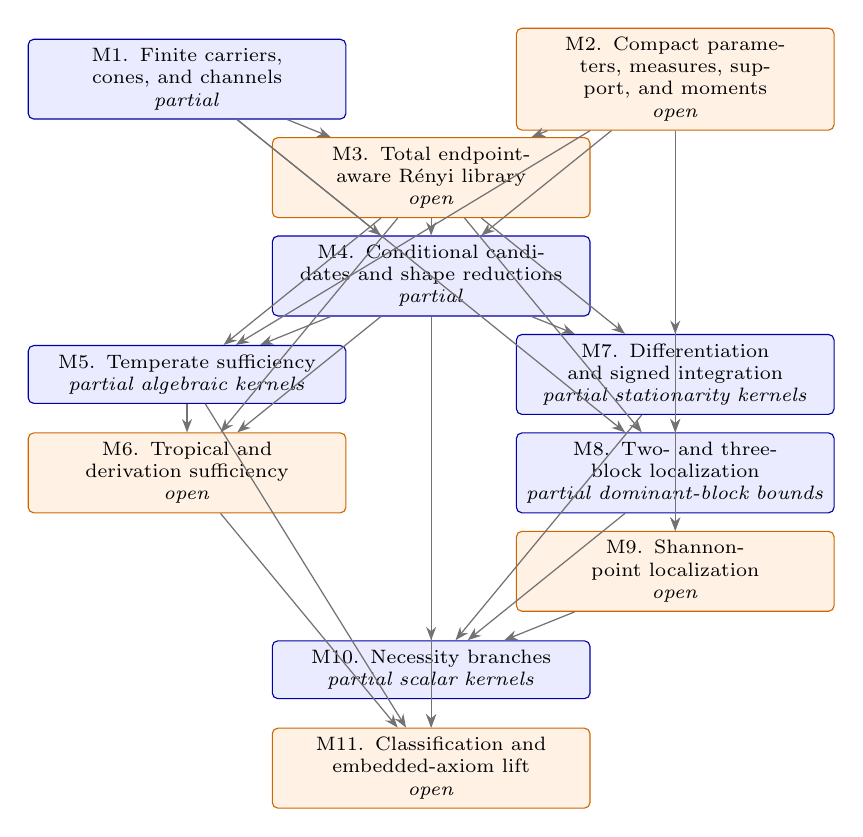
\begin{tikzpicture}[
      x=1cm,y=1cm,
      dep/.style={-{Stealth[length=1.7mm]},draw=black!55,line width=.45pt},
      partial/.style={draw=blue!65!black,fill=blue!8,rounded corners=2pt,
        align=center,font=\scriptsize,minimum height=7mm,text width=38mm},
      open/.style={draw=orange!80!black,fill=orange!10,rounded corners=2pt,
        align=center,font=\scriptsize,minimum height=7mm,text width=38mm}]
    \node[partial] (m1) at (-3.1,0) {M1. Finite carriers, cones, and channels\\\emph{partial}};
    \node[open]    (m2) at ( 3.1,0) {M2. Compact parameters, measures, support, and moments\\\emph{open}};
    \node[open]    (m3) at (0,-1.25) {M3. Total endpoint-aware R\'enyi library\\\emph{open}};
    \node[partial] (m4) at (0,-2.50) {M4. Conditional candidates and shape reductions\\\emph{partial}};
    \node[partial] (m5) at (-3.1,-3.75) {M5. Temperate sufficiency\\\emph{partial algebraic kernels}};
    \node[open]    (m6) at (-3.1,-5.00) {M6. Tropical and derivation sufficiency\\\emph{open}};
    \node[partial] (m7) at ( 3.1,-3.75) {M7. Differentiation and signed integration\\\emph{partial stationarity kernels}};
    \node[partial] (m8) at ( 3.1,-5.00) {M8. Two- and three-block localization\\\emph{partial dominant-block bounds}};
    \node[open]    (m9) at ( 3.1,-6.25) {M9. Shannon-point localization\\\emph{open}};
    \node[partial] (m10) at (0,-7.50) {M10. Necessity branches\\\emph{partial scalar kernels}};
    \node[open]    (m11) at (0,-8.75) {M11. Classification and embedded-axiom lift\\\emph{open}};

    \draw[dep] (m1) -- (m3);
    \draw[dep] (m2) -- (m3);
    \draw[dep] (m1) -- (m4);
    \draw[dep] (m2) -- (m4);
    \draw[dep] (m3) -- (m4);
    \draw[dep] (m2) -- (m5);
    \draw[dep] (m3) -- (m5);
    \draw[dep] (m4) -- (m5);
    \draw[dep] (m3) -- (m6);
    \draw[dep] (m4) -- (m6);
    \draw[dep] (m5) -- (m6);
    \draw[dep] (m2) -- (m7);
    \draw[dep] (m3) -- (m7);
    \draw[dep] (m4) -- (m7);
    \draw[dep] (m1) -- (m8);
    \draw[dep] (m2) -- (m8);
    \draw[dep] (m3) -- (m8);
    \draw[dep] (m7) -- (m8);
    \draw[dep] (m7) -- (m9);
    \draw[dep] (m8) -- (m9);
    \draw[dep] (m4) -- (m10);
    \draw[dep] (m7) -- (m10);
    \draw[dep] (m8) -- (m10);
    \draw[dep] (m9) -- (m10);
    \draw[dep] (m4) -- (m11);
    \draw[dep] (m5) -- (m11);
    \draw[dep] (m6) -- (m11);
    \draw[dep] (m10) -- (m11);
  \end{tikzpicture}
  \caption{Condensed formalization dependency graph.  An arrow
  \(A\to B\) means that blueprint layer \(B\) is planned to depend on
  layer \(A\).  Colours report translation status, not mathematical truth.}
  \label{fig:lean-dependency-graph}
\end{figure}

The repository also contains Graphviz and SVG versions of the same condensed
graph.  A separate declaration-level dependency index retains the individual
Lean names that are intentionally omitted from
Figure~\ref{fig:lean-dependency-graph}.

\subsection{Statement correspondence}
\label{app:lean-correspondence}

The status ``proved and kernel checked'' means that the named Lean declaration
has the blueprint statement's full conclusion.  ``Partial algebraic kernel''
means that it checks a genuine calculation used by the manuscript statement
but does not prove that statement's full measure-theoretic or asymptotic
conclusion.  ``Not formalized'' means that no Lean theorem with the manuscript's
conclusion is present.  Definitions are marked separately from proved
propositions.

% Statement ledger for the blueprint's Sections 4--5 and final assembly.
% This fragment is included by lean-formalization-appendix.tex.

\providecommand{\BlueprintStatement}[2]{%
  \texttt{\detokenize{#1}}: \emph{#2}}
\providecommand{\LeanDecl}[1]{\texttt{\detokenize{#1}}}

\small
\begin{longtable}{>{\raggedright\arraybackslash}p{0.35\textwidth}
                  >{\raggedright\arraybackslash}p{0.42\textwidth}
                  >{\raggedright\arraybackslash}p{0.15\textwidth}}
\caption{Statement-by-statement correspondence for blueprint Sections 4--5
and final assembly.}
\label{tab:blueprint-statement-correspondence}\\
\toprule
Manuscript statement & Lean declaration & Status\\
\midrule
\endfirsthead
\toprule
Manuscript statement & Lean declaration & Status\\
\midrule
\endhead
\bottomrule
\endfoot

\BlueprintStatement{lem:origin-extension}{Extension from the punctured cone}
  & \LeanDecl{ConditionalEntropy.originExtension} & Proved and kernel checked\\
\BlueprintStatement{lem:punctured-cone-convex}{Convexity of the punctured nonnegative cone}
  & \LeanDecl{ConditionalEntropy.puncturedConeConvex} & Proved and kernel checked\\
\BlueprintStatement{lem:composition-rule}{Monotone composition rule}
  & \LeanDecl{ConditionalEntropy.compositionRule} & Proved and kernel checked\\
\BlueprintStatement{lem:cone-composition-rule}{Monotone composition on the punctured cone}
  & \LeanDecl{ConditionalEntropy.coneCompositionRule} & Proved and kernel checked\\
\BlueprintStatement{lem:finite-holder}{Finite H\"older inequality}
  & --- & Not formalized\\
\BlueprintStatement{lem:power-curvature}{Power-mean curvature}
  & --- & Not formalized\\
\BlueprintStatement{lem:parameter-power-curvature}{Compactified power-mean bridge}
  & --- & Not formalized\\
\BlueprintStatement{def:hessian-quad}{Hessian quadratic form}
  & --- & Not formalized\\
\BlueprintStatement{lem:hessian-sign-criterion}{Hessian sign criterion}
  & --- & Not formalized\\
\BlueprintStatement{lem:real-rpow-calculus}{Positive-base real-power calculus}
  & --- & Not formalized\\
\BlueprintStatement{lem:monomial-curvature}{Curvature of an affine monomial}
  & \LeanDecl{ConditionalEntropy.monomialCurvature};
    \LeanDecl{ConditionalEntropy.monomialCurvature_eq_neg_variance};
    \LeanDecl{ConditionalEntropy.monomialCurvature_nonpos_of_nonneg};
    \LeanDecl{ConditionalEntropy.coefficient_mem_Icc_of_curvature_nonpos};
    \LeanDecl{ConditionalEntropy.monomialCurvature_pos_of_negative_coefficient};
    \LeanDecl{ConditionalEntropy.two_positive_stationary_witness};
    \LeanDecl{ConditionalEntropy.negativeTemperate_two_coefficient_curvature}
  & Partial algebraic kernel\\
\BlueprintStatement{lem:finite-support-enumeration}{Enumeration of a finite probability support}
  & --- & Not formalized\\
\BlueprintStatement{lem:finite-support-dirac}{Finite-support measure decomposition}
  & --- & Not formalized\\
\BlueprintStatement{prop:finite-sufficiency}{Finite-support sufficiency}
  & \LeanDecl{ConditionalEntropy.positiveTemperate_coefficients_nonnegative};
    \LeanDecl{ConditionalEntropy.negativeTemperate_two_coefficient_curvature}
  & Partial algebraic kernel\\
\BlueprintStatement{prop:general-sufficiency}{General temperate sufficiency}
  & \LeanDecl{ConditionalEntropy.isConcave_of_pointwise_tendsto};
    \LeanDecl{ConditionalEntropy.isConvex_of_pointwise_tendsto};
    \LeanDecl{ConditionalEntropy.conditioning_monotone_of_concave};
    \LeanDecl{ConditionalEntropy.conditioning_antitone_of_convex}
  & Partial algebraic kernel\\
\BlueprintStatement{cor:finite-t-sufficiency}{Finite-$t$ sufficiency}
  & \LeanDecl{ConditionalEntropy.positiveTemperate_coefficients_nonnegative};
    \LeanDecl{ConditionalEntropy.negativeTemperate_two_coefficient_curvature};
    \LeanDecl{ConditionalEntropy.conditioning_monotone_of_concave};
    \LeanDecl{ConditionalEntropy.conditioning_antitone_of_convex}
  & Partial algebraic kernel\\
\BlueprintStatement{prop:negative-tropical-sufficiency}{Negative tropical sufficiency}
  & \LeanDecl{ConditionalEntropy.isQuasiConvex_of_pointwise_tendsto}
  & Partial algebraic kernel\\
\BlueprintStatement{lem:positive-tropical-component}{Positive tropical component formula}
  & --- & Not formalized\\
\BlueprintStatement{prop:positive-tropical-sufficiency}{Positive tropical sufficiency}
  & \LeanDecl{ConditionalEntropy.isStronglyQuasiConcave_of_pointwise_tendsto}
  & Partial algebraic kernel\\
\BlueprintStatement{def:derivation-family}{Derivation polymorphic family}
  & --- & Not formalized\\
\BlueprintStatement{prop:derivation-sufficiency}{Derivation sufficiency}
  & --- & Not formalized\\
\BlueprintStatement{def:signed-column-functions}{Signed-measure column functions}
  & --- & Not formalized\\
\BlueprintStatement{def:signed-witness-predicates}{Positive and negative signed witnesses}
  & --- & Not formalized\\
\BlueprintStatement{lem:signed-witness-bridge}{Scaling, total variation, support, and atoms of witnesses}
  & --- & Not formalized\\
\BlueprintStatement{lem:signed-scalar-column-bridge}{Signed-scalar bridge to the candidate column functions}
  & --- & Not formalized\\
\BlueprintStatement{def:finite-param}{Embedding a finite real order}
  & --- & Not formalized\\
\BlueprintStatement{def:positive-line-data}{Positive multiplicative line data}
  & --- & Not formalized\\
\BlueprintStatement{def:positive-line-raw}{Raw multiplicative line}
  & --- & Not formalized\\
\BlueprintStatement{def:positive-line-predicate}{Positivity predicate for a line}
  & --- & Not formalized\\
\BlueprintStatement{lem:line-positive-zero}{The base point of a positive line is positive}
  & --- & Not formalized\\
\BlueprintStatement{def:line-cone}{Proof-carrying cone versions of a positive line}
  & --- & Not formalized\\
\BlueprintStatement{def:positive-line-prob}{Total normalized line}
  & --- & Not formalized\\
\BlueprintStatement{def:scalar-qcvx-on}{Scalar quasiconvexity on a set}
  & \LeanDecl{ConditionalEntropy.IsQuasiConvex}
  & Partial algebraic kernel\\
\BlueprintStatement{lem:cone-affine-line-bridge}{Restricting cone curvature to a positive affine line}
  & --- & Not formalized\\
\BlueprintStatement{def:entropy-line}{Entropy line}
  & --- & Not formalized\\
\BlueprintStatement{def:entropy-line-first}{First entropy line derivative}
  & --- & Not formalized\\
\BlueprintStatement{def:entropy-line-second}{Second entropy line derivative}
  & --- & Not formalized\\
\BlueprintStatement{def:escort-weight}{Escort weight}
  & --- & Not formalized\\
\BlueprintStatement{def:effective-line-velocity}{Effective line velocity}
  & --- & Not formalized\\
\BlueprintStatement{def:escort-mean}{Escort mean}
  & \LeanDecl{ConditionalEntropy.weightedMean}
  & Partial algebraic kernel\\
\BlueprintStatement{def:escort-second}{Escort second moment}
  & \LeanDecl{ConditionalEntropy.weightedSecondMoment}
  & Partial algebraic kernel\\
\BlueprintStatement{def:escort-variance}{Escort variance}
  & \LeanDecl{ConditionalEntropy.weightedVariance}
  & Partial algebraic kernel\\
\BlueprintStatement{def:fixed-max-coordinate}{Fixed maximal-coordinate condition}
  & --- & Not formalized\\
\BlueprintStatement{lem:positivity-intervals}{Common positivity and maximal-coordinate intervals}
  & --- & Not formalized\\
\BlueprintStatement{def:iterated-deriv}{Iterated one-variable derivative}
  & --- & Not formalized\\
\BlueprintStatement{def:lambda-deriv}{Iterated derivative in the second variable}
  & --- & Not formalized\\
\BlueprintStatement{def:alpha-lambda-deriv}{Mixed parameter--line derivative}
  & --- & Not formalized\\
\BlueprintStatement{def:removable-shannon-quotient}{Removable Shannon quotient}
  & --- & Not formalized\\
\BlueprintStatement{lem:parameterized-removable-quotient}{Parameterized removable quotient at the Shannon point}
  & --- & Not formalized\\
\BlueprintStatement{lem:signed-integral-differentiate-twice}{Twice differentiating a finite signed-measure integral}
  & --- & Not formalized\\
\BlueprintStatement{def:shannon-line-slope}{Shannon line slope}
  & --- & Not formalized\\
\BlueprintStatement{lem:exact-derivatives}{Exact entropy derivatives}
  & --- & Not formalized\\
\BlueprintStatement{def:integrated-entropy-line}{Integrated entropy along a line}
  & --- & Not formalized\\
\BlueprintStatement{def:signed-log-phi-line}{Signed logarithmic column line}
  & --- & Not formalized\\
\BlueprintStatement{lem:signed-line-column-bridge}{Exact bridge from line kernels to signed column functions}
  & --- & Not formalized\\
\BlueprintStatement{lem:differentiate-integral}{Differentiation through the parameter integral}
  & --- & Not formalized\\
\BlueprintStatement{lem:null-thresholds}{Null thresholds}
  & --- & Not formalized\\
\BlueprintStatement{lem:two-upper-null-thresholds}{Two finite null thresholds between upper parameters}
  & --- & Not formalized\\
\BlueprintStatement{lem:support-strict-integral}{Support gives strict weighted mass}
  & --- & Not formalized\\
\BlueprintStatement{lem:scalar-measure-support}{Scalar measure support and null points}
  & --- & Not formalized\\
\BlueprintStatement{def:block-index}{Finite dependent block carrier}
  & --- & Not formalized\\
\BlueprintStatement{def:block-vector}{Constant-on-block vector}
  & --- & Not formalized\\
\BlueprintStatement{def:block-data}{Asymptotic block data}
  & --- & Not formalized\\
\BlueprintStatement{lem:block-count-pos}{Positive block counts}
  & --- & Not formalized\\
\BlueprintStatement{def:block-carrier-nonempty}{Nonempty block-carrier instance}
  & --- & Not formalized\\
\BlueprintStatement{def:block-index-nonempty}{Nonempty arbitrary block index}
  & --- & Not formalized\\
\BlueprintStatement{def:block-max}{Maximum of a nonempty block vector}
  & --- & Not formalized\\
\BlueprintStatement{def:block-line-data}{Typed block line}
  & --- & Not formalized\\
\BlueprintStatement{def:block-kernels}{Block exponents, escort weights, and derivative kernels}
  & --- & Not formalized\\
\BlueprintStatement{lem:block-vector-formulas}{Block-vector finite-sum formulas}
  & --- & Not formalized\\
\BlueprintStatement{lem:rounding}{Rounding estimates}
  & --- & Not formalized\\
\BlueprintStatement{lem:dominant-block}{Dominant-block escort estimate}
  & \LeanDecl{ConditionalEntropy.dominantBlock_first};
    \LeanDecl{ConditionalEntropy.dominantBlock_second}
  & Partial algebraic kernel\\
\BlueprintStatement{lem:near-shannon-dominant}{Near-Shannon cancellation for a dominant block}
  & --- & Not formalized\\
\BlueprintStatement{lem:large-alpha-tail}{Large-order tail bound}
  & --- & Not formalized\\
\BlueprintStatement{def:block-limit-kernels}{Pointwise limit kernels for a block family}
  & --- & Not formalized\\
\BlueprintStatement{prop:block-limit-passage}{Uniform passage to the block limit}
  & --- & Not formalized\\
\BlueprintStatement{def:special-block-data}{Specialized block data and signed truncations}
  & --- & Not formalized\\
\BlueprintStatement{def:special-block-top-unique}{Unique top blocks for the special families}
  & --- & Not formalized\\
\BlueprintStatement{def:block-dominance-maps}{Total two-block and three-block dominance maps}
  & --- & Not formalized\\
\BlueprintStatement{lem:two-block-dominance-package}{Exact two-block dominance package}
  & --- & Not formalized\\
\BlueprintStatement{lem:three-block-dominance-package}{Exact three-block dominance package}
  & --- & Not formalized\\
\BlueprintStatement{lem:two-order-one-dominance}{Unique order-one block for the two-block family}
  & --- & Not formalized\\
\BlueprintStatement{lem:three-order-one-dominance}{Unique order-one block for the three-block family}
  & --- & Not formalized\\
\BlueprintStatement{def:block-log-g-kernels}{Block logarithmic and norm-free kernels}
  & --- & Not formalized\\
\BlueprintStatement{lem:compact-uniform-eval}{Evaluation of compact-uniform convergence}
  & --- & Not formalized\\
\BlueprintStatement{lem:compact-uniform-add}{Addition closure for compact-uniform convergence}
  & --- & Not formalized\\
\BlueprintStatement{lem:compact-uniform-singleton}{Evaluation on a singleton}
  & --- & Not formalized\\
\BlueprintStatement{lem:subtype-uniform-error-bridge}{Subtype bridge for uniform signed-integral errors}
  & --- & Not formalized\\
\BlueprintStatement{lem:block-curve-kernel-bridge}{Block curve--kernel bridge}
  & --- & Not formalized\\
\BlueprintStatement{lem:block-g-kernel-integrals}{Block (G)-kernels are signed kernel integrals}
  & --- & Not formalized\\
\BlueprintStatement{lem:block-log-mass-limit}{Block logarithmic-mass splitting and limit}
  & --- & Not formalized\\
\BlueprintStatement{lem:block-log-mass-continuity}{Continuity of logarithmic block-mass kernels}
  & --- & Not formalized\\
\BlueprintStatement{lem:block-kernel-regularity}{Linearity and continuity of the block kernels}
  & --- & Not formalized\\
\BlueprintStatement{def:two-block-limits}{Two-block limit polynomials}
  & --- & Not formalized\\
\BlueprintStatement{def:three-block-limits}{Three-block cells and limit polynomials}
  & --- & Not formalized\\
\BlueprintStatement{lem:two-block-limit-integral-eval}{Evaluation of the two-block limit integrals}
  & --- & Not formalized\\
\BlueprintStatement{lem:three-block-limit-integral-eval}{Evaluation of the three-block limit integrals}
  & --- & Not formalized\\
\BlueprintStatement{prop:block-localisation}{Two-block and three-block localisation}
  & --- & Not formalized\\
\BlueprintStatement{prop:two-block-localisation}{Two-block localisation interface}
  & --- & Not formalized\\
\BlueprintStatement{prop:three-block-localisation}{Three-block localisation interface}
  & --- & Not formalized\\
\BlueprintStatement{def:shannon-data}{Shannon block data}
  & --- & Not formalized\\
\BlueprintStatement{lem:shannon-q-pos}{Positivity of the complementary Shannon weight}
  & --- & Not formalized\\
\BlueprintStatement{lem:shannon-log-scale-pos}{Positivity of the Shannon logarithmic scale}
  & --- & Not formalized\\
\BlueprintStatement{lem:shannon-count-pos}{Positive Shannon block counts}
  & --- & Not formalized\\
\BlueprintStatement{def:shannon-index-nonempty}{Nonempty Shannon index and block representative}
  & --- & Not formalized\\
\BlueprintStatement{def:shannon-line-data}{Shannon line and its escort}
  & --- & Not formalized\\
\BlueprintStatement{lem:shannon-top-unique-at-zero}{The third Shannon block is strictly maximal at the base point}
  & --- & Not formalized\\
\BlueprintStatement{def:shannon-kernels}{Named Shannon kernels}
  & --- & Not formalized\\
\BlueprintStatement{lem:shannon-curve-kernel-bridge}{Shannon curve--kernel bridge}
  & --- & Not formalized\\
\BlueprintStatement{lem:shannon-kernel-integral-bridge}{Shannon derivative--integral and logarithmic splitting bridge}
  & --- & Not formalized\\
\BlueprintStatement{lem:shannon-kernel-regularity}{Linearity and continuity of the Shannon kernels}
  & --- & Not formalized\\
\BlueprintStatement{lem:shannon-dedicated-escort}{Dedicated Shannon escort, compact-region, and tail estimates}
  & --- & Not formalized\\
\BlueprintStatement{def:shannon-remainder}{Shannon main term and uniform remainder}
  & --- & Not formalized\\
\BlueprintStatement{lem:uniform-shannon-expansion}{Uniform Shannon expansion}
  & --- & Not formalized\\
\BlueprintStatement{lem:shannon-neighbourhood}{Uniform control near the Shannon point}
  & --- & Not formalized\\
\BlueprintStatement{def:remove-signed-atom}{Signed atom and its removal}
  & --- & Not formalized\\
\BlueprintStatement{lem:remove-signed-atom}{Removing a signed atom}
  & --- & Not formalized\\
\BlueprintStatement{lem:signed-witness-integral-bridge}{Witness atoms and the positive lower truncation}
  & --- & Not formalized\\
\BlueprintStatement{lem:shannon-log-mass}{Shannon-block logarithmic mass derivatives}
  & --- & Not formalized\\
\BlueprintStatement{def:shannon-localization-targets}{Shannon localization targets}
  & --- & Not formalized\\
\BlueprintStatement{prop:shannon-localisation}{Shannon-point localisation}
  & --- & Not formalized\\
\BlueprintStatement{def:normalized-curvature}{Normalized scalar-line curvature}
  & --- & Not formalized\\
\BlueprintStatement{lem:log-curvature-identity}{Logarithmic curvature identity}
  & --- & Not formalized\\
\BlueprintStatement{lem:log-curvature-obstruction}{Logarithmic curvature limit obstruction}
  & --- & Not formalized\\
\BlueprintStatement{def:stationarity-package}{Stationarity convergence package}
  & --- & Not formalized\\
\BlueprintStatement{lem:stationarity-correction}{Exact stationarity correction}
  & \LeanDecl{ConditionalEntropy.stationarityCorrection_dot};
    \LeanDecl{ConditionalEntropy.stationarityCorrection_tendsto}
  & Partial algebraic kernel\\
\BlueprintStatement{lem:quasiconvex-second}{Stationary curvature of a quasi-convex function}
  & \LeanDecl{ConditionalEntropy.not_quasiConvex_of_strict_midpoint_peak}
  & Partial algebraic kernel\\
\BlueprintStatement{lem:typed-log-curvature-contradiction}{Typed curvature contradiction from logarithmic kernels}
  & \LeanDecl{ConditionalEntropy.not_concave_of_strict_midpoint_valley};
    \LeanDecl{ConditionalEntropy.not_convex_of_strict_midpoint_peak}
  & Partial algebraic kernel\\
\BlueprintStatement{lem:corrected-stationary-line-obstruction}{Corrected stationary-line obstruction}
  & \LeanDecl{ConditionalEntropy.stationarityCorrection_dot};
    \LeanDecl{ConditionalEntropy.stationarityCorrection_tendsto};
    \LeanDecl{ConditionalEntropy.not_quasiConvex_of_strict_midpoint_peak}
  & Partial algebraic kernel\\
\BlueprintStatement{prop:positive-necessity}{Positive-measure obstruction}
  & \LeanDecl{ConditionalEntropy.negative_tail_concavity_obstruction};
    \LeanDecl{ConditionalEntropy.excessive_lower_moment_concavity_obstruction};
    \LeanDecl{ConditionalEntropy.shannon_atom_concavity_obstruction};
    \LeanDecl{ConditionalEntropy.positiveTemperate_shannon_atom_zero};
    \LeanDecl{ConditionalEntropy.positiveTemperate_no_upper_moment};
    \LeanDecl{ConditionalEntropy.positiveTemperate_lowerMoment_le_one};
    \LeanDecl{ConditionalEntropy.positiveTemperate_necessary}
  & Partial algebraic kernel\\
\BlueprintStatement{cor:positive-temperate-probability-necessity}{Positive temperate necessity for probability measures}
  & \LeanDecl{ConditionalEntropy.positiveTemperate_necessary}
  & Partial algebraic kernel\\
\BlueprintStatement{prop:negative-shannon-obstruction}{A Shannon atom excludes upper support}
  & --- & Not formalized\\
\BlueprintStatement{def:negative-truncations}{Positive lower and upper truncations}
  & --- & Not formalized\\
\BlueprintStatement{lem:negative-truncation-bridge}{Negative-witness truncation identities}
  & --- & Not formalized\\
\BlueprintStatement{prop:truncated-moment}{Truncated-moment obstruction}
  & \LeanDecl{ConditionalEntropy.two_positive_stationary_witness};
    \LeanDecl{ConditionalEntropy.negativeTemperate_truncated_moment};
    \LeanDecl{ConditionalEntropy.negativeTemperate_exceptional_moment}
  & Partial algebraic kernel\\
\BlueprintStatement{prop:one-upper-point}{At most one upper support point}
  & \LeanDecl{ConditionalEntropy.two_positive_stationary_witness};
    \LeanDecl{ConditionalEntropy.negativeTemperate_atMostOneUpperCell}
  & Partial algebraic kernel\\
\BlueprintStatement{prop:negative-temperate-necessity}{Complete negative temperate necessity}
  & \LeanDecl{ConditionalEntropy.negativeTemperate_exceptional_moment};
    \LeanDecl{ConditionalEntropy.negativeTemperate_atMostOneUpperCell}
  & Partial algebraic kernel\\
\BlueprintStatement{cor:negative-temperate-probability-necessity}{Negative temperate necessity for probability measures}
  & \LeanDecl{ConditionalEntropy.negativeTemperate_exceptional_moment};
    \LeanDecl{ConditionalEntropy.negativeTemperate_atMostOneUpperCell}
  & Partial algebraic kernel\\
\BlueprintStatement{prop:negative-tropical-necessity}{Complete negative tropical necessity}
  & \LeanDecl{ConditionalEntropy.negativeTropical_moment_nonnegative};
    \LeanDecl{ConditionalEntropy.negativeTropical_exceptional_moment}
  & Partial algebraic kernel\\
\BlueprintStatement{def:prob-as-pos-cone}{Probability support as a positive cone vector}
  & --- & Not formalized\\
\BlueprintStatement{lem:prob-as-pos-cone-identities}{Probability-to-cone identities}
  & --- & Not formalized\\
\BlueprintStatement{lem:prob-support-nonempty}{A probability vector has nonempty positive support}
  & --- & Not formalized\\
\BlueprintStatement{lem:same-support-decomposition}{Decomposition inside a simplex face}
  & --- & Not formalized\\
\BlueprintStatement{lem:probability-eq-dirac-zero}{Probability supported at zero is the zero Dirac measure}
  & --- & Not formalized\\
\BlueprintStatement{prop:positive-tropical-necessity}{Only the support-rank measure survives}
  & --- & Not formalized\\
\BlueprintStatement{def:derivation-column-function}{Derivation column function}
  & --- & Not formalized\\
\BlueprintStatement{prop:derivation-necessity}{Derivation necessity}
  & \LeanDecl{ConditionalEntropy.positive_tail_derivation_obstruction};
    \LeanDecl{ConditionalEntropy.derivation_no_positive_upper_tail};
    \LeanDecl{ConditionalEntropy.derivation_necessary}
  & Partial algebraic kernel\\
\BlueprintStatement{thm:necessity-bundle}{All necessary parameter conditions}
  & \LeanDecl{ConditionalEntropy.positiveTemperate_necessary};
    \LeanDecl{ConditionalEntropy.negativeTemperate_exceptional_moment};
    \LeanDecl{ConditionalEntropy.negativeTropical_exceptional_moment};
    \LeanDecl{ConditionalEntropy.derivation_necessary}
  & Partial algebraic kernel\\
\BlueprintStatement{thm:main-classification}{Complete parameter classification}
  & --- & Not formalized\\
\BlueprintStatement{def:conditional-entropy-axioms}{Conditional-entropy axiom bundle}
  & --- & Not formalized\\
\BlueprintStatement{lem:embedding-lift}{Embedding lift of fixed-row monotonicity}
  & --- & Not formalized\\
\BlueprintStatement{cor:all-conditional-entropy-axioms}{Admissible candidates satisfy the complete axiom bundle}
  & --- & Not formalized\\

\end{longtable}
\normalsize



\end{document}
